% Clase del documento
\documentclass[12pt,twoside,titlepage]{report}





%%%%%%%%%%%%%%%%%%%%%%% Paquetes %%%%%%%%%%%%%%%%%%%%%%%

\usepackage[a4paper,bindingoffset=3mm,bottom=35mm]{geometry}


% Usad \usepackage[dvips]{graphicx} o \usepackage[pdftex]{graphicx} (no ambos)
%\usepackage[dvips]{graphicx} %%% para LaTeX. Las figuras deben estar en formato eps

\usepackage[colorlinks=true,pdftex]{hyperref}   %%% Opcional. Para incluir marcadores y enlaces en el pdf
\usepackage[pdftex]{graphicx}  %%% para pdflatex. Las figuras pueden estar en pdf, jpg, svg y otros formatos


\usepackage[spanish]{babel}


%\usepackage[latin1]{inputenc} % Usad en WinEdt/MikTex
\usepackage[utf8]{inputenc} % Usad en overleaf

%\usepackage[T1]{fontenc}


% Algunos paquetes útiles

\usepackage{amsmath,amssymb}
\usepackage{hyperref}
\usepackage{color}
\usepackage{afterpage}
\usepackage{paralist}
\usepackage{array}
\usepackage{enumerate}
\usepackage{paralist}
\usepackage{enumitem}
\usepackage{float}
\usepackage{setspace}
\usepackage{listings}
\usepackage{algorithm}
\usepackage{algorithmic}
\usepackage{fancyhdr}
\usepackage{rotating}
\usepackage{multirow}
\usepackage{fancyvrb}
\usepackage{wrapfig}


% Otros paquetes

\usepackage{quotchap}
\usepackage{lipsum}


%%%%%%%%%%%%%%%%%%%%%%%%%%%%%%%%%%%%%%%%%%%%%%%%%%%%%%%%






%%%%%%%%%%%%%%%%%%%%%%% Definiciones básicas %%%%%%%%%%%%%%%%%%%%%%%

\newcommand{\nombreautor}{Oscar Nydza Nicpoñ}
\newcommand{\nombretutor}{Juan Manuel Serrano Hidalgo}
\newcommand{\titulotrabajo}{Comparativa entre las API de Spark en Scala y Python}
\newcommand{\escuela}{Escuela Técnica Superior\\de Ingeniería Informática}
\newcommand{\escuelalargo}{Escuela Técnica Superior de Ingeniería Informática}
\newcommand{\universidad}{Universidad Rey Juan Carlos}
\newcommand{\fecha}{Fecha}
\newcommand{\grado}{Grado en Ingeniería de Computadores}
\newcommand{\curso}{Curso 2021-2022}
\newcommand{\logoUniversidad}{logoURJC.pdf} % logoURJC.eps
\newcommand{\quotes}[1]{``#1''}

%%%%%%%%%%%%%%%%%%%%%%%%%%%%%%%%%%%%%%%%%%%%%%%%%%%%%%%%%%%%%%%%%%%%






%%%%%%%%%%%%%%%%%%%%%%%%% Otras definiciones %%%%%%%%%%%%%%%%%%%%%%%%%%

% Definiciones de colores (para hidelinks)
\definecolor{BlueLink}{rgb}{0.165,0.322,0.745}
\definecolor{PinkLink}{rgb}{0.8,0.22,0.5}
\definecolor{gray}{rgb}{0.6,0.6,0.6}


% Enlaces
\hypersetup{hidelinks,pageanchor=true,colorlinks,citecolor=PinkLink,urlcolor=black,linkcolor=BlueLink}


\newcommand\blankpage{%
    \newpage
    \null
    \thispagestyle{empty}%
    %\addtocounter{page}{-1}%
    \newpage}


% Texto referencias
\addto{\captionsspanish}{\renewcommand{\bibname}{Bibliografía}}

% Texto Índice de tablas
\addto\captionsspanish{
\def\tablename{Tabla}
\def\listtablename{\'{I}ndice de tablas}
}


\floatname{algorithm}{Algoritmo}

\newfloat{algorithm}{t}{lop}


%\newenvironment{pseudocodigo}[1][htb]
%  {\renewcommand{\algorithmcfname}{Pseudocódig}% Update algorithm name
%   \begin{algorithm}[#1]%
%  }{\end{algorithm}}
  
%%%%%%%%%%%%%%%%%%%%%%%%%%%%%%%%%%%%%%%%%%%%%%%%%%%%%%%%%%%%%%%%%%%%





%%%%%%%%%%%%%%%%%%%%%%% Estilo de código (en Python) %%%%%%%%%%%%%%%%%%%%%%%

\definecolor{bg}{rgb}{0.95,0.95,0.95}
\definecolor{mydeepteal}{rgb}{0.16,0.22,0.23}
\definecolor{myteal}{rgb}{0.31,0.44,0.46}
\definecolor{mymediumteal}{rgb}{0.41,0.58,0.60}

\DeclareFixedFont{\ttb}{T1}{txtt}{bx}{n}{12} % for bold
\DeclareFixedFont{\ttm}{T1}{txtt}{m}{n}{12}  % for normal


%\newcommand*{\FormatDigit}[1]{\textcolor{mydeepteal}{#1}}
\newcommand*{\FormatDigit}[1]{\textcolor{black}{#1}}

% Python style for highlighting
\newcommand\mypythonstyle{\lstset{
language=Python,
basicstyle=\ttfamily\small,
%basicstyle=\linespread{1.0}\footnotesize\ttm,
otherkeywords={self},             % Add keywords here
keywordstyle=\bfseries\ttfamily\color{myteal},
%keywordstyle=\ttb\color{myteal},
commentstyle=\itshape\color{myteal},
stringstyle=\color{mydeepteal},
emph={MyClass,__init__},          % Custom highlighting
emphstyle=\ttb\color{mydeepteal},    % Custom highlighting style
% Any extra options here
showstringspaces=false,            %
backgroundcolor=\color{bg},
rulecolor = \color{bg},
%identifierstyle=\color{deepgreen},
breaklines=true,
numbers=left,
numbersep=5pt,
numberstyle=\tiny,
tabsize=4,
xleftmargin=1em,
frame = single,
framesep = 3pt,
framextopmargin=0pt,
framexbottommargin=0pt,
framexleftmargin=0pt,
framexrightmargin=0pt,
fontadjust=true,
basewidth=0.55em, % compactness of code
upquote=true,
}}

% Python environment
\lstnewenvironment{mypython}[1][]
{
\mypythonstyle
\lstset{#1}
}
{}

\newcommand\mypythonstylenormalinline{\lstset{
language=Python,
basicstyle=\ttfamily\normalsize,
%basicstyle=\linespread{1.0}\footnotesize\ttm,
otherkeywords={self},            % Add keywords here
keywordstyle=\bfseries\ttfamily\color{myteal},
%keywordstyle=\ttb\color{myteal},
commentstyle=\itshape\color{mymediumteal},
stringstyle=\color{mydeepteal},
emph={MyClass,__init__},          % Custom highlighting
emphstyle=\ttb\color{mydeepteal},    % Custom highlighting style
% Any extra options here
showstringspaces=false,            %
backgroundcolor=\color{bg},
rulecolor = \color{bg},
%identifierstyle=\color{deepgreen},
breaklines=false,
numbers=left,
numbersep=5pt,
numberstyle=\tiny,
tabsize=4,
xleftmargin=0em,
frame = single,
framesep = 3pt,
framextopmargin=0pt,
framexbottommargin=0pt,
framexleftmargin=0pt,
framexrightmargin=0pt,
fontadjust=true,
%basewidth=0.55em, % compactness of code
upquote=true,
}}

\newcommand\mypythoninline[1]{{\mypythonstylenormalinline\lstinline!#1!}}

%%%%%%%%%%%%%%%%%%%%%%%%%%%%%%%%%%%%%%%%%%%%%%%%%%%%%%%%%%%%%%%%%%%%%%%%%%%%%%

\usepackage{listings}

% "define" Scala
\lstdefinelanguage{scala}{
  morekeywords={abstract,case,catch,class,def,%
    do,else,extends,false,final,finally,%
    for,if,implicit,import,match,mixin,%
    new,null,object,override,package,%
    private,protected,requires,return,sealed,%
    super,this,throw,trait,true,try,%
    type,val,var,while,with,yield},
  otherkeywords={=>,<-,<\%,<:,>:,\#,@},
  sensitive=true,
  morecomment=[l]{//},
  morecomment=[n]{/*}{*/},
  morestring=[b]",
  morestring=[b]',
  morestring=[b]"""
}

\usepackage{color}
\definecolor{dkgreen}{rgb}{0,0.6,0}
\definecolor{gray}{rgb}{0.5,0.5,0.5}
\definecolor{mauve}{rgb}{0.58,0,0.82}

\lstset{frame=tb,
  language=scala,
  aboveskip=3mm,
  belowskip=3mm,
  showstringspaces=false,
  columns=flexible,
  basicstyle={\scriptsize\ttfamily},
  numbers=none,
  numberstyle=\tiny\color{gray},
  keywordstyle=\color{blue},
  commentstyle=\color{dkgreen},
  stringstyle=\color{mauve},
  frame=single,
  breaklines=true,
  breakatwhitespace=true
  tabsize=3
  basewidth=0.55em
}

\lstdefinelanguage{regex}{
	morekeywords={[, ], *, +, \^, ?},
	otherkeywords={$\backslash$},
	sensitive=true
}

%%%%%%%%%%%%%%%%%%%%%%%%%%%% Comandos definidos por el autor 

\newcommand{\transpuesta}{\mbox{\tiny $\mathsf{T}$}}









%%%%%%%%%%%%%%%%%%%%%%%%%%%%%%%%%%%%%%%%%%%%%%%%%%%%%%%%%%%%%%%%%%%%%%%
%                           Inicio del documento                       
%%%%%%%%%%%%%%%%%%%%%%%%%%%%%%%%%%%%%%%%%%%%%%%%%%%%%%%%%%%%%%%%%%%%%%%


\begin{document}

\pagestyle{plain}




%%%%%%%%%%%%%%%%%%%%%%%%%%%%%%%%%%%% Portada %%%%%%%%%%%%%%%%%%%%%%%%%%%%%%%%%%

%\pagenumbering{gobble}
%\pagenumbering{arabic}

% Universidad, Facultad
\begin{titlepage}
\selectlanguage{spanish}


% logo
\begin{center}
    \includegraphics[scale=0.7]{\logoUniversidad}
\end{center}

\bigskip

\begin{center}
\begin{LARGE}
\escuela \\
\end{LARGE}
\end{center}

\bigskip
\bigskip

% Grado
\begin{center}
\begin{large}
\textbf{\grado}\\
\end{large}
\end{center}

% Curso
\begin{center}
\begin{large}
\textbf{\curso}\\
\end{large}
\end{center}

\bigskip

\textbf{\begin{center}
\begin{large}
\textbf{Trabajo Fin de Grado}
\end{large}
\end{center}}

\bigskip
\bigskip
\bigskip

% Nombre del TFG
\begin{center}
\textbf{\begin{large}
\MakeUppercase{\titulotrabajo}\\
\end{large}}
\end{center}

% Nombre del autor
\vspace{\fill}
\begin{center}
\textbf{Autor: \nombreautor}\\ \smallskip
% Tutor
\textbf{Tutor: \nombretutor}\\
% Añadir segundo tutor si hubiera


\bigskip

% Fecha
%\textbf{\fecha}\\
\end{center}
\end{titlepage}


%%%%%%%%%%%%%%%%%%%%%%%% Opcional %%%%%%%%%%%%%%%%%%%%%%
%\blankpage

%\thispagestyle{empty}
%\begin{center}

% Nombre del trabajo
%\textbf{\begin{large}
%\MakeUppercase{\titulotrabajo}\\*
%\end{large}}
%\vspace*{0.2cm}
%\vspace{5cm}

% Nombre del autor y del tutor
%\large Autor: \nombreautor \\* \medskip
%\large Tutor: \nombretutor \\*

%\vfill

% Escuela, universidad y fecha
%\escuelalargo \\ \smallskip
%\universidad \\
%\vspace{1cm}
%\fecha \\

%\clearpage

%\end{center}
%%%%%%%%%%%%%%%%%%%%%%%%%%%%%%%%%%%%%%%%%%%%%%%%%%%%%%%%

\hypersetup{pageanchor=true}

\normalsize
\afterpage{\blankpage} % Se deben añadir página en blanco para que lo capítulos de la memoria o estas secciones introductorias empiecen en páginas impares

%%%%%%%%%%%%%%%%%%%%%%%%%%%%%%%%%%%%%%%%%%%%%%%%%%%%%%%%%%%%%%%%%%%%%%%%%%%%%%%





% Estilo de párrafo de los capítulos
\setlength{\parskip}{0.75em}
\renewcommand{\baselinestretch}{1.25}
% Interlineado simple
\spacing{1}

\pagenumbering{Roman}
\setcounter{page}{2}


%%%%%%%%%%%%%%%%%%%%%%%%% Agradecimientos o dedicatoria %%%%%%%%%%%%%%%%%%%%%%%%%%%

\chapter*{Agradecimientos}

Quiero dedicar este trabajo a todo el mundo que ha confiado en mí a lo largo de los años y que me ha apoyado en los momento más difíciles. En especial a mi madre, que ha demostrado tener más paciencia que nadie que haya conocido.

\afterpage{\blankpage}

%%%%%%%%%%%%%%%%%%%%%%%%%%%%%%%%%%%%%%%%%%%%%%%%%%%%%%%%%%%%%%%%%%%%%%%%%%%%%%%%%%%






%%%%%%%%%%%%%%%%%%%%%%%%%%%%%%%%%%%% Resumen %%%%%%%%%%%%%%%%%%%%%%%%%%%%%%%%%%%%%%

\chapter*{Resumen}

En este TFG vamos a ver cómo programar queries o peticiones a una fuente de datos local, ya sea en formato CSV o Parquet, usando Spark tanto en su API de Scala como de Python. Veremos los detalles que diferencian sintácticamente ambas API y cómo podríamos migrar peticiones de la API de Scala a la de Python. Tras esto, al ver que resulta relativamente arduo hacerlo a mano, desarrollaremos una serie de expresiones regulares con su respectiva expresión de sustitución que nos ayudará en el proceso de migración, y propondremos cómo se podría automatizar este proceso.

Veremos también los resultados de nuestras peticiones e intentaremos sacar conclusiones de ellas. Para ello usaremos la librería Plotly, que nos generará gráficos para ayudar visualmente a la tarea.

Tras esto pasaremos a comparar el rendimiento de ambas API, y veremos cómo el conjunto de datos utilizado no ha sido el más adecuado. Habiendo justificado el por qué, se realizará una última petición a un conjunto de datos que encaja mejor con la API que estamos usando. Veremos el rendimiento en tareas necesarias para ejecutar las peticiones, tiempos de tarea y uso de memoria. Además, se comparará el rendimiento entre formatos de entrada: usaremos ficheros CSV, Parquet sin particionar y Parquet simular cierto paralelismo y demostrar cómo ayuda a la hora de usar estas API.

\mbox{} \bigskip

\noindent \textbf{Palabras clave}:
\begin{compactitem}
    \item Spark
    \item Python
    \item Scala
\end{compactitem}

\afterpage{\blankpage}

%%%%%%%%%%%%%%%%%%%%%%%%%%%%%%%%%%%%%%%%%%%%%%%%%%%%%%%%%%%%%%%%%%%%%%%%%%%%%%%%%%%





%%%%%%%%%%%%%%%%%%%%%%%%%%%%%%%%%%%% Índices %%%%%%%%%%%%%%%%%%%%%%%%%%%%%%%%%%%%

% Estilo de párrafo de los Índices
\setlength{\parskip}{1pt}
\renewcommand{\baselinestretch}{1}
\renewcommand{\contentsname}{Índice de contenidos}


% Índice de contenidos
\tableofcontents
\afterpage{\blankpage}

% Índice de tablas (OPCIONAL)
%\listoftables
%\afterpage{\blankpage}
%\addcontentsline{toc}{chapter}{\noindent \listtablename}

% Índice de figuras (OPCIONAL)
\listoffigures
\afterpage{\blankpage}
\addcontentsline{toc}{chapter}{\listfigurename}

% Índice de códigos/algoritmos (OPCIONAL).   El término "Códigos" se puede cambiar por "Métodos", "Funciones", "Algoritmos", etc.
%\renewcommand\lstlistlistingname{Códigos}
%\renewcommand\lstlistingname{Código}
%\renewcommand\lstlistlistingname{Índice de códigos}

%\lstlistoflistings
%\afterpage{\blankpage}
\addcontentsline{toc}{chapter}{\lstlistlistingname}


% En este documento (de momento) no se ha considerado incluir un índice de algoritmos/pseudocódigos, como el que aparece en \ref{AdditionalLouvain}

%%%%%%%%%%%%%%%%%%%%%%%%%%%%%%%%%%%%%%%%%%%%%%%%%%%%%%%%%%%%%%%%%%%%%%%%%%%%%%%%%%%





%%%%%%%%%%%%%%%%%%%%%%% Cabeceras y pies de página (Opcional) %%%%%%%%%%%%%%%%%%%%%%%

%\setlength{\headheight}{15.2pt}
\pagestyle{fancy}


\renewcommand{\chaptermark}[1]{\markboth{Capítulo \thechapter.\ #1}{}}

\pagestyle{fancy}
\fancyhf{}
\fancyhead[LO]{\leftmark}
\fancyhead[RO]{}
\fancyhead[RE]{\nouppercase\rightmark}
\fancyhead[LE]{}
\fancyfoot[C]{\thepage}

%%%%%%%%%%%%%%%%%%%%%%%%%%%%%%%%%%%%%%%%%%%%%%%%%%%%%%%%%%%%%%%%%%%%%%%%%%%%%%%%%%%%






%%%%%%%%%%%%%%%%%%%%%%%%%%%%%% Capítulos de la memoria %%%%%%%%%%%%%%%%%%%%%%%%%%%%%



% Capítulo 1
\chapter{Introducción}
\newpage

%%%%%%%%%%%%%%%%%%%%%%%%%%%%%%%%%%%%%%%%%%%%%%%%%%%%%%%%%%%%%%%%%%%%%%%%%%

% Estilo resto de páginas
\pagestyle{fancy}


% Estilo de párrafo de los capítulos
\setlength{\parskip}{0.75em}
\renewcommand{\baselinestretch}{1.25}
% Interlineado simple
\spacing{1}
% Numeración contenido
\pagenumbering{arabic}
\setcounter{page}{1}

%%%%%%%%%%%%%%%%%%%%%%%%%%%%%%%%%%%%%%%%%%%%%%%%%%%%%%%%%%%%%%%%%%%%%%%%%%

Spark está definido como \quotes{un motor multilenguaje para ejecutar tareas de ingeniería de datos, ciencia de datos y \textit{machine learning} en máquinas con un solo nodo o en \textit{clusters}}\footnote{\url{https://spark.apache.org/}}. En resumen, se utiliza en entornos de \textit{big data}, ya que el paralelismo que ofrece otorga enormes ventajas que iremos descubriendo.

Mediante el uso de APIs disponibles en distintos lenguajes es posible programar peticiones a fuentes de datos de forma eficiente y relativamente sencilla, ya que tiene una sintaxis que resulta familiar si se ha trabajado lenguajes de consultas como SQL. De hecho, es posible utilizar únicamente este estilo de programación. Sin embargo, también proporciona otros métodos para realizar este procesado de datos mediante el uso de funciones como si de un lenguaje funcional se tratara.

A la hora de desplegar un entorno que use Spark como motor para el procesado de datos, nos puede surgir la duda de cuál de las distintas API podemos utilizar. A simple vista puede resultar complicado: dejando de lado la API de SQL, tenemos APIs disponibles en Scala, Python, Java y R. Sería interesante tener información sobre su rendimiento antes de tomar una decisión que puede costar mucho dinero a nivel de empresa.

Es por esto último que nos vamos a centrar en dos APIs: Scala Spark y PySpark. Se han elegido expresamente dado que una es \quotes{nativa} y otra es \quotes{no nativa}, que son básicamente las dos categorías de APIs disponibles. Por un lado como nativas tenemos a la de Java y Scala y como no nativas a la de Python y R.

Este trabajo consistirá en intentar establecer una serie de comparativas y tratar de llegar a una conclusión lo más clara posible sobre cuál de estas dos es la más eficiente dentro del entorno limitado del que dispondremos.


% \afterpage{\blankpage} % puede generar problema en índice de contenidos
% \newpage


% Capítulo 2
\chapter{Objetivos}
\newpage

El principal objetivo de este Trabajo de Fin de Grado realizar una comparativa entre las API de Spark de Scala y de Python. Al ser un objetivo amplio, vamos a especificar objetivos más pequeños y concretos:


\subsubsection{Objetivo 1}

Vamos a utilizar un conjunto de datos del dominio de la Fórmula 1 ya que tenemos varias preguntas que necesitan respuesta. Estas son:

\begin{compactitem}
  \item Cuál ha sido el piloto más consistente en la temporada 2012. Se calculará la diferencia entre el tiempo medio de todas las vueltas de cada piloto ese periodo de tiempo en concreto y la media de sus vueltas más rápidas.
  \item Cuál ha sido el mejor piloto de la historia calculando valores estadísticos como el total de carreras ganadas, el total de títulos, el número de vueltas lideradas, el número de primeras posiciones en clasificación, número de vueltas rápidas, etc. Todo ello relativo a su periodo de actividad.
  \item Cuál ha sido el fabricante más dominante en un periodo de tiempo concreto.
  \item Análisis de temporada por pilotos: se calcularán diversas medidas estadísticas para cada piloto. Por ejemplo, el total de podios, el porcentaje de carreras en las que se ha acabado en podio, la media de posiciones perdidas y ganadas por carrera, el número de vueltas lideradas, etc.
  \item Cuál ha sido la temporada más interesante para el espectador, teniendo en cuenta métricas como el número de adelantamientos, más cambios de líder en la clasificación general, etc.
\end{compactitem}

Para responder a estas cuestiones tendremos que realizar una serie de queries utilizando ambas API, aprendiendo en el camino cómo programarlas y viendo las diferencias y similitudes entre ambas.

\subsubsection{Objetivo 2}

Sería también útil encontrar una manera de poder visualizar estos resultados obtenidos de forma gráfica. Para ello usaremos la librería Plotly, que, como ya veremos, nos proporciona una manera sencilla de obtener gráficos a partir de datos.

\subsubsection{Objetivo 3}

Buscaremos la manera de migrar queries programadas en Scala Spark a PySpark. Esto nos permitirá ver mejor las diferencias entre las API a la hora de programarlas. Intentaremos buscar también la manera de automatizar este proceso.

\subsubsection{Objetivo 4}

Comparar el rendimiento de ambas API a nivel de tiempos de ejecución y uso de recursos. Utilizaremos la Spark UI para obtener estas métricas y veremos cuál se comporta mejor en un entorno lo más igualado posible.


\section{Metodología de trabajo}

En esta sección vamos a ver las herramientas que se van a usar, ya que se puede considerar un objetivo secundario el aprendizaje de las mismas.

Lo primero que tendremos que aprender será a programar funciones sencillas en Scala. Ya que es un lenguaje que no se enseñó en Ingeniería de Computadores durante los años en los que fui alumno, considero importante obtener un nivel básico de conocimientos sobre su uso antes de lanzarse de lleno a usar su API de Spark.

Lo mismo podríamos decir de Python, sin embargo este lenguaje sí se cursó en la asignatura Lenguajes de Programación y se obtuvo un nivel suficiente como usuario, así que no lo veo como un objetivo.

Tendremos que aprender también a utilizar cuadernos Jupyter para desarrollar código tanto en Scala como Python, ya que nos permitirá avanzar más rápidamente en las fases iniciales del proyecto al facilitar la depuración de las queries que se van a programar.

A la hora de migrar queries usaremos expresiones regulares de búsqueda y sustitución. En concreto para ello se usará \texttt{sed}, y teorizaremos sobre cómo podríamos utilizar scripts de Bash para automatizar el proceso.

Para describir la fuente de datos usaremos DataGrip de JetBrains, que nos permitirá obtener diagramas Entidad-Relación de nuestro conjunto de datos de forma más sencilla.

También usaremos Git como sistema de control de versiones tanto para todo el código desarrollado como para esta misma memoria, que se va a escribir usando \LaTeX.

Por último, será necesario aprender \LaTeX para desarrollar esta misma memoria.



% Capítulo 3
\chapter{Descripción Informática}
\label{chap:contenidos}
\newpage

En este capítulo se va a abordar la parte más técnica del proyecto. 

En primer lugar veremos una descripción detallada de los datos de los que disponemos, proporcionando ejemplos y un diagrama Entidad-Relación en el que podremos ver cómo están relacionados los distintos ficheros de entrada.

Luego pasaremos a centrarnos en la programación de queries: primero en Scala Spark y luego en PySpark. Se describirá a grandes rasgos qué queremos conseguir y el por qué. Tras esto, nos centraremos en el proceso de construcción de queries desde un plano más técnico. En concreto, veremos cómo se programa una query en cada API, dejando el resto para los apéndices.

Por último veremos el proceso de migración de queries desde Scala a Python, centrándonos en las diferencias entre APIs y trataremos de facilitar lo máximo este proceso mediante el desarrollo de una serie de expresiones regulares.

\section{Fuentes de datos}

En esta sección vamos a ver en profundidad cómo es el conjunto de datos que se ha escogido para la realización de este proyecto. Veremos también varios formatos: CSV y Parquet. Nos centraremos en las diferencias entre ellos y pondremos el punto de mira en cómo podríamos cambiar del primero al segundo, en teoría más eficiente.

\subsection{Formato CSV}

Como se mencionó brevemente en el apartado de Objetivos, se ha utilizado un conjunto de datos de la Fórmula 1 que fue obtenido del enlace disponible en la bibliografía \cite{datasource}. Concretamente, este conjunto de datos tiene 13 tablas que proporcionan información sobre distintos aspectos de esta competición. Estas tablas son:

\begin{compactitem}
  \item \texttt{circuits}
  \item \texttt{constructor$\_$results}
  \item \texttt{constructor$\_$standings}
  \item \texttt{constructors}
  \item \texttt{driver$\_$standings}
  \item \texttt{lap$\_$times}
  \item \texttt{pit$\_$stops}
  \item \texttt{qualifying}
  \item \texttt{races}
  \item \texttt{results}
  \item \texttt{seasons}
  \item \texttt{status}
  \item \texttt{drivers}
\end{compactitem}

Todas estas tablas están interrelacionadas como se puede ver en el diagrama Entidad-Relación que se presenta a continuación:

\begin{figure}[H]
  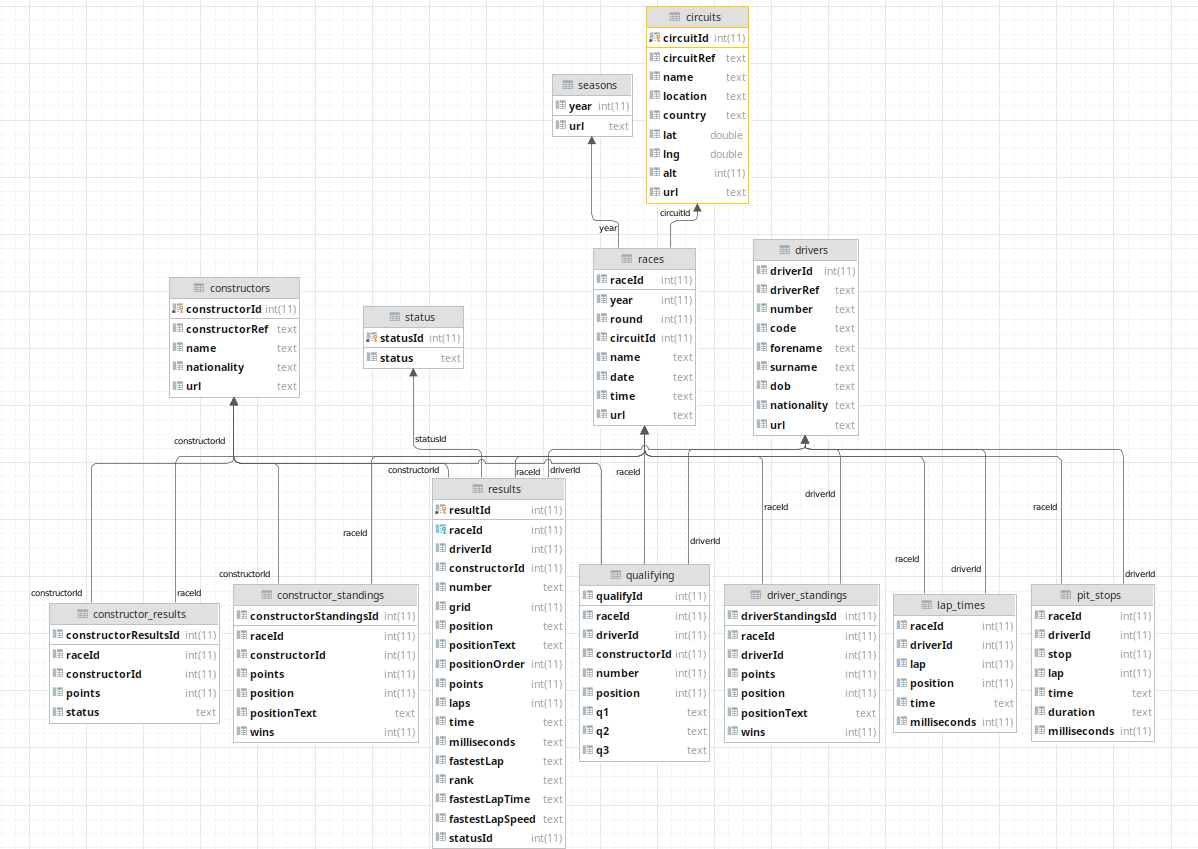
\includegraphics[scale=0.4]{dataset_visualization.png}
  \centering
  \caption{Diagrama Entidad-Relación}
  \label{fig:datavisualization}
  \centering
\end{figure}


\subsubsection{Tabla \texttt{circuits}}

Esta tabla contiene información sobre todos los circuitos en los que se ha llevado a cabo un Gran Premio. Las columnas más interesantes son el nombre del circuito, una referencia textual y la localización. 

\begin{figure}[H]
  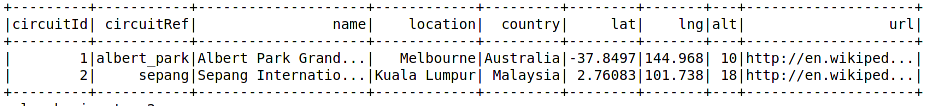
\includegraphics[scale=0.4]{circuits_table.png}
  \centering
  \caption{Tabla circuits}
  \label{fig:circuits}
  \centering
\end{figure}

\subsubsection{Tabla \texttt{constructor$\_$results}}

Esta tabla nos proporciona información sobre los resultados de las carreras en base a los constructores. 

\begin{figure}[H]
  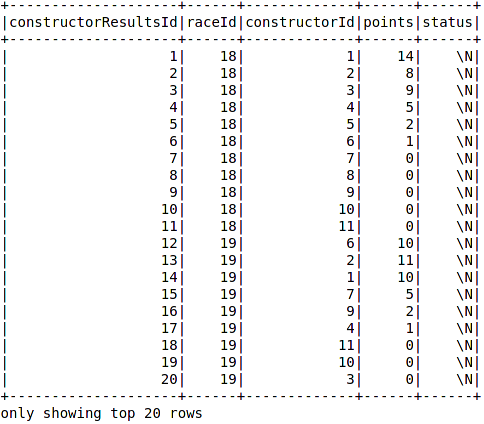
\includegraphics[scale=0.4]{constructor_results_table.png}
  \centering
  \caption{Tabla constructor$\_$results}
  \label{fig:constructorres}
  \centering
\end{figure}


\subsubsection{Tabla \texttt{constructor$\_$standings}}

Esta tabla contiene información sobre la clasificación de constructores. Como particularidad, tiene una entrada por carrera y constructor participante. Por tanto, podríamos ver cómo ha ido cambiando la clasificación de constructores a lo largo del campeonato.

Las columnas más interesantes son el identificador de la carrera, identificador del constructor, los puntos, la posición en la clasificación y las victorias hasta ese punto. 


\begin{figure}[H]
  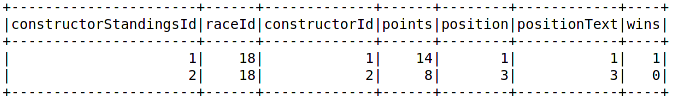
\includegraphics[scale=0.4]{constructor_standings_table.png}
  \centering
  \caption{Tabla constructor$\_$standings}
  \label{fig:constructorstands}
  \centering
\end{figure}

\subsubsection{Tabla \texttt{constructors}}

Esta tabla contiene información sobre los distintos constructores que han participado en algún campeonato mundial de Fórmula 1. Las columnas más interesantes son el id de constructor, la referencia, el nombre del constructor y la nacionalidad. 

\begin{figure}[H]
  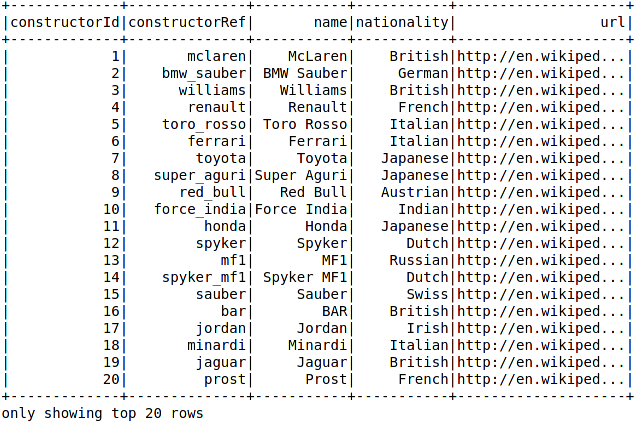
\includegraphics[scale=0.4]{constructors_table.png}
  \centering
  \caption{Tabla constructors}
  \label{fig:constructors}
  \centering
\end{figure}


\subsubsection{Tabla \texttt{driver$\_$standings}}

Similar a la tabla de clasificación de constructores, pero para pilotos. Tenemos las mismas columnas, salvo que en lugar de tener un id de constructor, lo tenemos de piloto. 


\begin{figure}[H]
  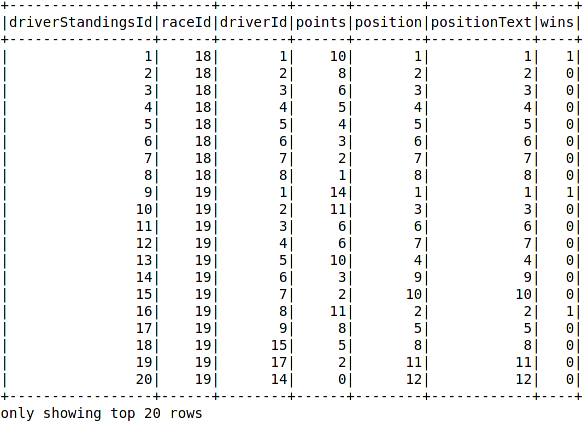
\includegraphics[scale=0.4]{driver_standings_table.png}
  \centering
  \caption{Tabla driver$\_$standings}
  \label{fig:drivstands}
  \centering
\end{figure}


\subsubsection{Tabla \texttt{lap$\_$times}}

Esta tabla es una de las más interesantes, ya que nos da todos los tiempos de vuelta de todos los pilotos desde que hay registros. Esto es, desde parte de 1996 y 1997 al completo.

Las columnas más llamativas podrían ser el id de carrera, el de piloto, la vuelta en cuestión, la posición y el tiempo en milisegundos. 

\begin{figure}[H]
  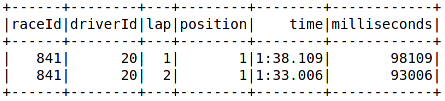
\includegraphics[scale=0.4]{lap_times_table.png}
  \centering
  \caption{Tabla lap$\_$times}
  \label{fig:laptimestab}
  \centering
\end{figure}

\subsubsection{Tabla \texttt{pit$\_$stops}}

Esta tabla contiene información de las paradas en boxes. Las columnas más interesantes son los id de carrera y piloto, el índice de parada (si es la primera, segunda, etc), la vuelta en la que se hace y la duración en milisegundos. 

\begin{figure}[H]
  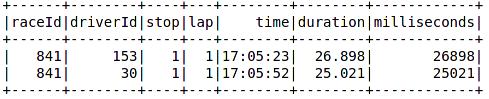
\includegraphics[scale=0.5]{pit_stop_table.png}
  \centering
  \caption{Tabla pit$\_$stops}
  \label{fig:pitstops}
  \centering
\end{figure}

\subsubsection{Tabla \texttt{qualifying}}

Esta tabla nos da información sobre los resultados de todas las rondas de clasificación. La columnas más interesantes son la posición final y los tiempos en Q1, Q2 y Q3. 

\begin{figure}[H]
  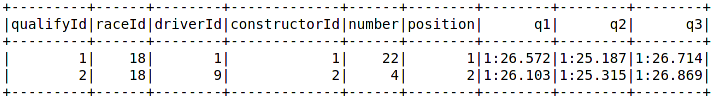
\includegraphics[scale=0.4]{qualifying_table.png}
  \centering
  \caption{Tabla qualifying}
  \label{fig:quali}
  \centering
\end{figure}


\subsubsection{Tabla \texttt{races}}

Esta tabla contiene información sobre todas las carreras celebradas en la historia de la competición. Contiene columnas como el id del circuito, el nombre del Gran Premio, la fecha y el año en el que se celebró. Esta última quizá sea la más útil de todo el dataset, ya que es la única forma de filtrar las carreras o los resultados por temporada. 

\begin{figure}[H]
  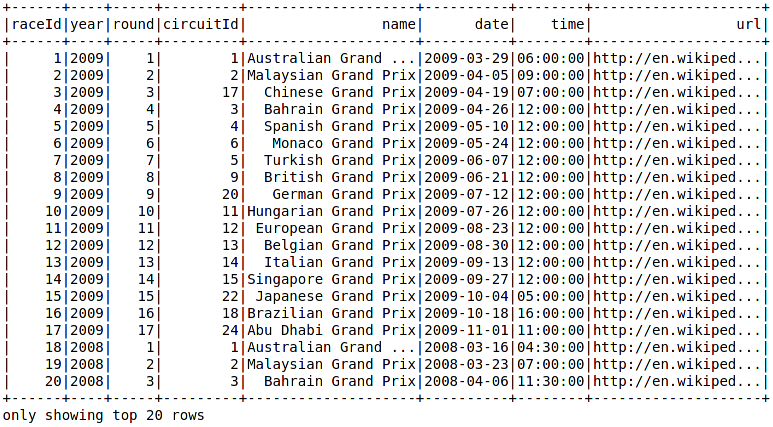
\includegraphics[scale=0.4]{races_table.png}
  \centering
  \caption{Tabla races}
  \label{fig:races}
  \centering
\end{figure}

\subsubsection{Tabla \texttt{results}}

Esta tabla es similar a la de resultados por constructor, pero para pilotos. Es la tabla más completa de todas, ya que nos proporciona una entrada por piloto y carrera con información relevante de cómo se ha desarrollado la misma. Las columnas más interesantes pueden ser la posición de salida y la posición final, los puntos ,las vueltas dadas, la vuelta más rápida, la velocidad más rápida y, en el caso de que haya habido algún incidente, el id del estado. 

\begin{figure}[H]
  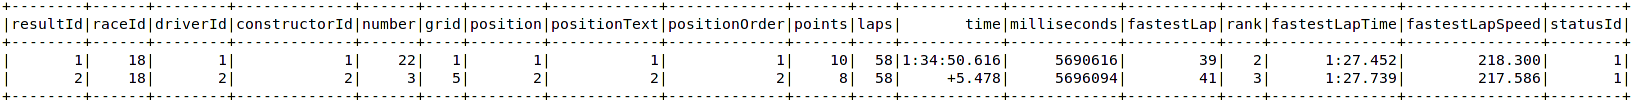
\includegraphics[scale=0.27]{results_table.png}
  \centering
  \caption{Tabla results}
  \label{fig:resultstab}
  \centering
\end{figure}

\subsubsection{Tabla \texttt{seasons}}

Quizá se trate de la tabla menos útil, ya que solamente contiene una columna con el año y otra con una url a un artículo de Wikipedia para cada entrada. 

\begin{figure}[H]
  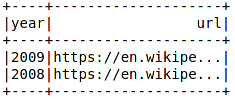
\includegraphics[scale=0.5]{season_table.png}
  \centering
  \caption{Tabla seasons}
  \label{fig:seasonstable}
  \centering
\end{figure}


\subsubsection{Tabla \texttt{status}}

Esta tabla nos da información sobre los estados en los que ha podido acabar la carrera un piloto determinado. Contiene un identificador y el estado en cuestión. 

\begin{figure}[H]
  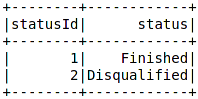
\includegraphics[scale=0.5]{status_table.png}
  \centering
  \caption{Tabla status}
  \label{fig:statustable}
  \centering
\end{figure}

\subsubsection{Tabla \texttt{drivers}}

Contiene información sobre todos los pilotos que han competido a lo largo de la historia. En concreto la información más relevante puede ser el nombre y apellido, el código, la fecha de nacimiento y la nacionalidad. 

\begin{figure}[H]
  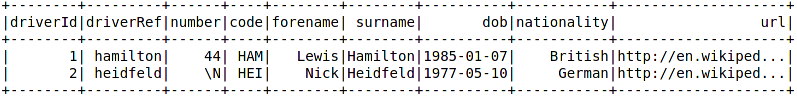
\includegraphics[scale=0.5]{driver_table.png}
  \centering
  \caption{Tabla drivers}
  \label{fig:driverstable}
  \centering
\end{figure}


\subsubsection{Tabla \texttt{drivers constructor season}} \label{drivconstseasontabexplanation}

Esta tabla no estaba originalmente en el conjunto de datos, pero resultó necesario establecer una relación entre cada piloto con su constructor en cada temporada. Principalmente se necesita para poder hacer comparativas entre pilotos del mismo equipo o bien de forma global o bien por temporadas. 

Esta tabla se creó a partir de la tabla \texttt{races}, que contiene la temporada y la tabla \texttt{results}, que contiene tanto el constructor como el piloto. Se hizo la intersección de estas tablas mediante la columna identificadora de la carrera. El código es el siguiente:


\begin{lstlisting}
val raceSeasonMap = spark.read.format("csv")
  .option("header", "true")
  .option("sep", ",")
  .load("../data/races.csv")
  .select("raceId", "year")

spark.read.format("csv")
  .option("header", "true")
  .option("sep", ",")
  .load("../data/results.csv")
  .join(raceSeasonMap, Seq("raceId"), "left")
  .select("year", "driverId", "constructorId")
  .dropDuplicates()
  .repartition(1)
  .write.format("csv")
  .option("header", "true")
  .save("../data/drivers_constr_season.csv")
\end{lstlisting}

Para escribir la tabla en disco, primero tenemos que utilizar \texttt{repartition} para que el resultado final quede en un solo archivo CSV. Después especificamos el formato y si queremos las cabeceras o no, y proporcionamos el directorio donde queremos que quede guardado.

Finalmente la tabla contiene información tal que:

\begin{figure}[H]
  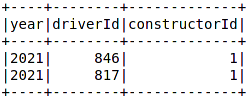
\includegraphics[scale=0.4]{driv_const_ssn_table.png}
  \centering
  \caption{Tabla auxiliar piloto-constructor-temporada}
  \label{fig:driv_const_ssn_table}
  \centering
\end{figure}

\subsection{Formato Parquet}

También utilizaremos el formato de ficheros Parquet como alternativa a CSV ya que nos puede otorgar beneficios a la hora de ejecutar nuestras queries, mejorando el rendimiento tanto en tiempos de ejecución como en tamaño de datos de entrada leídos.

Parquet es un formato que, además de los propios datos, almacena metadatos y realiza ciertos indexados y optimizaciones para que se ocupe el menor espacio posible en disco. Además, podemos particionar la tabla según ciertas columnas clave, permitiendo que Spark, tras hacer sus optimizaciones propias del proceso, sepa qué archivos tiene que leer y cuáles no. Un ejemplo de cómo se ve una fuente de datos de entrada en disco puede ser el siguiente:

\begin{figure}[H]
	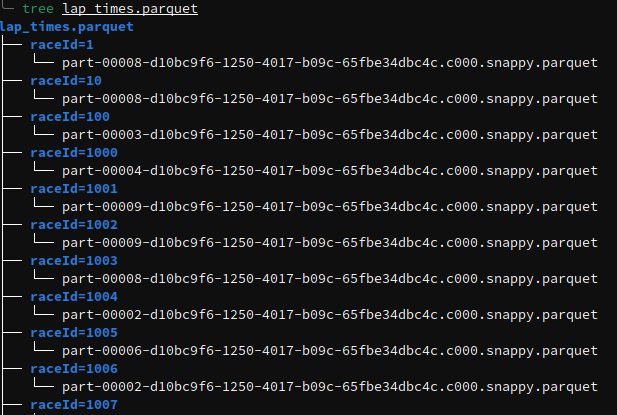
\includegraphics[scale=0.35]{treeparquet.png}
	\centering
	\caption{Archivos Parquet en disco}
	\label{fig:parquetendisco}
	\centering
\end{figure}

Podemos ver que la tabla en cuestión está particionada según el campo \texttt{raceId}, y que tenemos una subcarpeta por cada valor que toma. Dentro de cada subcarpeta está ya el archivo Parquet, que contiene los datos para ese \texttt{raceId}. Si tuviéramos más datos, tendríamos más archivos dentro de las subcarpetas.

Teóricamente leer datos que están en formato Parquet usando Spark debería ser más eficiente ya que no se lee la tabla completa, al contrario que con los CSV.

Más adelante se van a comparar tres formatos de entrada: CSV, Parquet particionado y Parquet sin particionar. Originalmente el conjunto de datos venía en formato CSV, así que no necesitamos realizar ningún procesamiento extra para conseguirlo. Sin embargo, los otros dos formatos van a necesitar un poco de trabajo adicional.

Convertir los tipos de entrada no conlleva mucho trabajo a nivel de código, pero puede resultar enrevesado ya que se necesita conocer el conjunto de datos y realizar un análisis previo al particionado, debido a que es posible realizar un particionado \quotes{malo} si no se tiene en cuenta cómo van a quedar los datos almacenados en disco.

Para llevar a cabo este particionado se ha desarrollado una función que dado un nombre de tabla y un nombre de columna realiza la conversión y escribe los datos en disco:

\begin{lstlisting}
def toParquet(tableName: String, partitionCol: String): Unit = {
	val ini = spark.read.format("csv")
		.option("header", "true")
		.option("sep", ",")
		.load(s"../data/$tableName.csv")
		
	if (partitionCol == "noPartitionCol") {
		ini.write.mode("overwrite")
			.parquet(s"../data/parquet/$tableName.parquet")
	} else {
		ini.repartition(col(partitionCol))
			.write.mode("overwrite")
			.partitionBy(partitionCol)
			.parquet(s"../data/parquet/$tableName.parquet")
	}
}
\end{lstlisting}

El detalle que determina el particionado es, en el \texttt{else}, las operaciones \texttt{repartition} y \texttt{partitionBy}.

Por comodidad, se ha creado otra función distinta que dado un nombre de tabla lo escribe como Parquet sin particionar:

\begin{lstlisting}
def toParquetNoPart(tableName: String): Unit = {
	spark.read.format("csv")
		.option("header", "true")
		.option("sep", ",")
		.load(s"../data/$tableName.csv")
		.write.mode("overwrite")
		.parquet(s"../data/parquetnopart/$tableName.parquet")
}
\end{lstlisting}

Con estas dos funciones definidas, una lista con los nombres de las tablas (\texttt{files}) y un mapa que establezca una relación entre nombre de tabla y columna de particionado (\texttt{partCol}), podemos convertir todas las tablas de entrada de golpe si ejecutamos lo siguiente:

\begin{lstlisting}
files.foreach(x => toParquet(x, partCol(x)))
\end{lstlisting}

O, en el caso de que queramos parquet sin particionar:

\begin{lstlisting}
files.foreach(x => toParquetNoPart(x))
\end{lstlisting}

Una vez tenemos todos los datos como deseamos solamente tendremos que cambiar las líneas en las que se leen los datos de entrada, de forma que si antes teníamos algo como:

\begin{lstlisting}
spark.read.format("csv")
	.option("header", "true")
	.option("sep", ",")
	.load("tablePath")
\end{lstlisting}

Ahora tenemos algo como:

\begin{lstlisting}
spark.read.parquet("tablePath")
\end{lstlisting}


\section{Programación de queries en Scala Spark}

En esta sección vamos a ver cómo se programan queries en la API de Scala, veremos principalmente la sintaxis y, al ser el primer apartado en el que se programe una query, se va a explicar detalladamente el proceso de creación de una query para Spark: nos detendremos en las funciones y veremos cómo usarlas para obtener los resultados buscados.

Como comenté anteriormente en forma de introducción a la sección, veremos un ejemplo y dejaremos el otro para el apéndice \ref{extrascala}.

Antes de entrar en materia cabe destacar que, debido a que vamos a usar distintas fuentes de entrada (CSV y Parquet), se va a abstraer la parte de la lectura de las fuentes de datos de la propia query, que se hará en una función que recibirá los \texttt{DataFrames} con los datos necesarios previos al procesado.

La función tendrá el siguiente aspecto:

\begin{lstlisting}
def queryEnCuestion(entrada1: DataFrame, entrada2: DataFrame, ...): DataFrame = {
	...
}
\end{lstlisting}

Y devolverá un \texttt{DataFrame} con los resultados obtenidos para luego poder visualizarlos, escribirlos o cualquier otra operación que veamos pertinente. El uso por tanto será el siguiente:

\begin{lstlisting}
queryEnCuestion(entradaLeida1, entradaLeida2, ...)
\end{lstlisting}

Es por esto que en la descripción de las queries se va a dar por asumido que tenemos los datos de entrada ya leídos, salvo la primera vez que hagamos una lectura, en cuyo caso se explicará en detalle.

\subsection{Piloto más consistente en un periodo concreto de tiempo}

En esta query intentaremos averiguar cuál ha sido el piloto más consistente en un periodo de tiempo dado, en este caso en la temporada 2012. Ya que este término puede resultar ambiguo, en concreto intentaremos averiguar qué piloto tuvo una menor diferencia entre la media de sus vueltas rápidas y la media de todas las vueltas de todos los Grandes Premios de este periodo de tiempo. Esto nos resultará especialmente interesante teniendo en cuenta que cuanto menor sea esta diferencia, más consistente habrá sido el piloto respecto a su mejor resultado.

Necesitaremos cruzar varias fuentes de datos: 

\begin{compactitem}
	\item \texttt{races.csv}
	\item \texttt{lap$\_$times.csv}
	\item \texttt{drivers.csv}
	\item \texttt{results.csv}
\end{compactitem}

Dicho esto, la query tiene el siguiente aspecto:

\begin{lstlisting}
def queryConsistencia(races:DataFrame, lap_times:DataFrame, drivers:DataFrame, results:DataFrame):DataFrame = {
	val driverWindow = Window.partitionBy("driverId")
	val seasonWindow = Window.partitionBy("year")
	
	
	val races_filtered = races
		.where(col("year") === 2012)
	
	val avg_lap_times = lap_times
		.withColumnRenamed("time", "lapTime")
		.join(races_filtered, Seq("raceId"), "right")
		.withColumn("milliseconds", col("milliseconds").cast(IntegerType))
		.withColumn("avgMs", avg(col("milliseconds")).over(driverWindow))
		.dropDuplicates("driverId")
		.select("driverId", "avgMs")
	
	val lapCount = lap_times
		.join(races_filtered, Seq("raceId"), "right")
		.withColumn("lapsPerDriver", count(col("lap")).over(driverWindow))
	
	val (distinctDrivers, allLaps) = lapCount
		.agg(
			countDistinct("driverID"),
			count(col("lap"))
		).as[(BigInt, BigInt)]
		.collect()(0)
	
	val avgLapsThisPeriod = allLaps.toInt / distinctDrivers.toInt
		
	val experiencedDrivers = lapCount
		.where(col("lapsPerDriver") >= avgLapsThisPeriod)
		.select("driverId")
		.distinct()
		.as[String]
		.collect()
	
	results.join(races, Seq("raceId"), "right")
		.na.drop(Seq("fastestLapTime"))
		.withColumn("fastestLapTimeMs", lapTimeToMsUDF(col("fastestLapTime")))
		.withColumn("avgFastestLapMs", avg(col("fastestLapTimeMs")).over(driverWindow))
		.dropDuplicates("driverId")
		.join(avg_lap_times, Seq("driverId"), "left")
		.withColumn("diffLapTimes", abs('avgMs - 'avgFastestLapMs).cast(IntegerType))
		.withColumn("avgDiff", msToLapTimeUDF(col("diffLapTimes").cast(IntegerType)))
		.where(col("driverId").isInCollection(experiencedDrivers))
		.join(drivers, "driverId")
		.withColumn("driver", concat(col("forename"), lit(" "), col("surname")))
		.select("driver", "avgDiff")
		.orderBy("avgDiff")
}
\end{lstlisting}

\subsubsection{Descripción detallada}

A continuación entramos en el detalle de la implementación de esta query.

Primero de todo, queremos leer las fuentes de datos para luego pasar el \texttt{DataFrame} a la función ya explicada. Para ello, ejecutamos las siguientes líneas de código:

\begin{lstlisting}
val races = spark.read.format("csv")
  .option("header", "true")
  .option("sep", ",")
  .load("data/races.csv")
\end{lstlisting}

En este caso leemos la tabla \texttt{races}. Como se puede observar, se utilizan un par de opciones de lectura. En nuestro caso, la fuente de datos contiene las cabeceras en la primera línea y cada dato está separado por una coma y por ello tenemos que especificarlo. Por último se proporciona el path relativo de la fuente de datos.

Si quisiéramos leer de un archivo Parquet, la sintaxis queda más simplificada:

\begin{lstlisting}
val races = spark.read.parquet("path_to_races_parquet")
\end{lstlisting}

Tras esto, ya dentro de nuestra función, se hace el filtro según las temporadas que se quieran usar. Para ello, ya que el periodo sobre el que se quiere obtener datos viene dado como tipo entero y simboliza la temporada, tenemos que convertir la columna \texttt{year} a tipo entero, ya que por defecto, al no especificar el esquema a la hora de leer, Spark intenta adivinar los tipos de cada columna. Es posible que detecte esa columna como tipo entero, pero conviene asegurar haciendo la conversión de tipos. Después de esto, llevamos a cabo el filtro. Al final, para obtener este \texttt{DataFrame} que utilizaremos más adelante se llevan a cabo las siguientes operaciones:

\begin{lstlisting}
val races_filtered = races
  .withColumn("year", col("year").cast(IntegerType))
  .where(col("year") === 2012)
\end{lstlisting}

De este trozo de código hay que comentar un par de aspectos. Primero, la conversión de tipos, que se hace al tipo \texttt{IntegerType}, y no a \texttt{Int}, como sería intuitivo hacer. Esto es porque Spark tiene una serie de tipos concretos para el tipo \texttt{Column}. Todos ellos se encuentran en el paquete \texttt{org.apache.spark.sql.types}, y es obligatorio su uso si se utiliza la función \texttt{cast}. También cabe destacar la función de DataFrame llamada \texttt{withColumn}, que se encuentra entre las más usadas, ya que permite añadir una columna al \texttt{DataFrame}. Crea una columna con el nombre que recibe como primer parámetro y con el valor que recibe en el segundo. En este caso, ya que la columna \texttt{year} ya existe, se sustituye la que había anteriormente con ese nombre.

El otro aspecto a comentar es el propio filtro. Se utiliza la función \texttt{where}, que cumple el mismo propósito que su equivalente en SQL. Como parámetro recibe una condición, que en nuestro caso querríamos que fuese que \quotes{la columna \texttt{year} sea igual al parámetro recibido, en este caso 2012}. Para esto podemos hacer una comparativa de la columna en cuestión con el valor deseado como si de un \texttt{if} se tratara.

Resumiendo, con estas pocas líneas de código hemos obtenido todas las carreras celebradas en el rango de temporadas que necesitamos. Más adelante se utilizará para filtrar los resultados de cada piloto y obtener solamente los que nos interesan. Merecía la pena pararse en este trocito de código ya que se repite en todas las queries en las que se requiere centrarse en un periodo concreto de tiempo.

Para realizar esta consulta vamos a necesitar varios \texttt{DataFrames} auxiliares además del recién explicado. En concreto, necesitaremos tener una cuenta de todas las vueltas que ha dado cada piloto en el periodo de tiempo establecido, además de la tabla \texttt{drivers} para completar la información final.

Para calcular todas las vueltas que ha dado cada piloto usaremos \texttt{lap$\_$times}. Le tendremos que aplicar el filtro de temporadas utilizando lo obtenido anteriormente y, por último, se hará el conteo. Todo ello se puede hacer de la siguiente manera:

\begin{lstlisting}
val lapCount = lap_times
  .join(races, Seq("raceId"), "right")
  .withColumn("lapsPerDriver", count(col("lap")).over(driverWindow))
\end{lstlisting}

Aquí vemos cómo se aplica el filtro de temporadas. Para ello hacemos la operación \texttt{join} con el DataFrame \texttt{races} obtenido anteriormente, sobre la columna \texttt{raceId} y de tipo \texttt{right}. En Spark SQL, existen varios tipos de intersecciones (join) que podemos realizar entre dos DataFrames:

\begin{compactitem}
  \item Inner Join.
  \item Full Outer Join.
  \item Left Outer Join
  \item Right Outer Join.
  \item Left Anti Join.
  \item Left Semi Join.
\end{compactitem}

Todos ellos definidos de la misma manera que en el Álgebra de Conjuntos.

Para nuestro caso particular, utilizaremos un Right Outer Join, ya que nos queremos quedar con las vueltas de las carreras definidas en \texttt{races}.

Tras esto, queremos obtener las vueltas que ha dado cada piloto en ese periodo de tiempo. Para ello, tenemos que utilizar la función \texttt{count} sobre la columna \texttt{lap}. Sin embargo, nos topamos con que, si hiciéramos eso (aparte de que el compilador no nos dejaría), necesitamos definir una ventana sobre la que operar.

Las ventanas son una parte muy útil de Spark que nos permiten centrarnos en cierta información agrupada de la forma que necesitemos. En nuestro caso, necesitamos contar las vueltas que ha dado cada piloto sin tener en cuenta las del resto y para ello necesitamos definir una ventana nueva (en nuestro caso se podría llamar \texttt{driverWindow}) que particione los datos por piloto. Esto lo hacemos de la siguiente manera:

\begin{lstlisting}
val driverWindow = Window.partitionBy("driverId") 
\end{lstlisting}

Utilizando esta ventana, la operación \texttt{count} se llevará a cabo un conteo distinto por cada \texttt{driverId} que haya. Si particionásemos los datos según varias columnas, se llevaría a cabo la operación en cuestión según cada valor único de esas columnas en conjunto, es decir, si hay alguna variación en alguna de ellas, se toma como una operación distinta.

Este \texttt{DataFrame} lo vamos a utilizar para definir cuáles son los pilotos más experimentados de este periodo de tiempo, que diremos que son los que han dado más de la media de vueltas por piloto. Para calcular esto y partiendo del \texttt{DataFrame} recién obtenido necesitamos conseguir dos valores: el número total de vueltas dadas entre todos los pilotos y el número de pilotos que han competido en este periodo de tiempo. Lo haremos de la siguiente manera:

\begin{lstlisting}
val (distinctDrivers, allLaps) = lapCount
  .agg(
    countDistinct("driverID"),
    count(col("lap"))
  ).as[(BigInt, BigInt)]
  .collect()(0)
\end{lstlisting}

Estos valores los obtendré en forma de tupla, en la que el valor de la izquierda será el número de pilotos y el de la derecha el número de vueltas. Cabe centrarse en la operación \texttt{agg}, que nos permite obtener un \texttt{DataFrame} cuyas columnas tendrán como valor el obtenido de las operaciones que definamos. En este caso, \texttt{countDistinct} que, como su nombre indica, cuenta los valores distintos de la columna \texttt{driverId} y \texttt{count}, que realiza un conteo de todas las entradas de la columna \texttt{lap}. Con \texttt{as} le definimos el tipo de datos que queremos obtener y con \texttt{collect}, obtenemos todos los valores del \texttt{DataFrame}. En este caso, como solo vamos a tener una entrada, y esta va a ser la única que necesitemos, hacemos un \texttt{collect()(0)}

Para calcular la media de vueltas por piloto en este periodo de tiempo, realizamos la siguiente operación:

\begin{lstlisting}
val avgLapsThisPeriod = allLaps.toInt / distinctDrivers.toInt
\end{lstlisting}

Con esta métrica podremos definir cuáles son los pilotos más experimentados de la siguiente manera:

\begin{lstlisting}
val experiencedDrivers = lapCount
  .where(col("lapsPerDriver") >= avgLapsThisPeriod)
  .select("driverId")
  .distinct()
  .as[String]
  .collect()
\end{lstlisting}

Con el \texttt{DataFrame} obtenido anteriormente, nos quedamos con los pilotos que tengan un número de vueltas superior o igual al índice calculado. Tras esto, nos quedamos solamente con los valores distintos la columna que indica el piloto y los obtenemos en forma de \texttt{List[String]} con las dos últimas operaciones para más adelante poder filtrar según ella.

Tras esto, querremos obtener la media de todas las vueltas que ha dado cada piloto. Para ello, usamos de nuevo la tabla \texttt{lap$\_$times}, en la que tenemos una columna llamada \texttt{milliseconds} y filtramos las temporadas que nos interesan. Para asegurar, convertimos esta columna a tipo entero y hacemos la media usando la ventana que creamos antes. Eliminamos los pilotos duplicados y nos quedamos con dos columnas: identificador de piloto y la media obtenida. El código queda tal que:

\begin{lstlisting}
val avgLapTimes = lap_times
  .withColumnRenamed("time", "lapTime")
  // filtro las vueltas de las carreras en el periodo de tiempo dado
  .join(races_filtered, Seq("raceId"), "right")
  .withColumn("milliseconds", col("milliseconds").cast(IntegerType))
  // media de tiempos de vuelta por piloto
  .withColumn("avgMs", avg(col("milliseconds")).over(driverWindow))
  .dropDuplicates("driverId")
  .select("driverId", "avgMs")
\end{lstlisting}


Finalmente, querríamos obtener un \texttt{DataFrame} que contenga dos columnas: el nombre del piloto y la diferencia ya mencionada anteriormente. Para ello, necesitamos usar la tabla \texttt{results} y dejar fuera las temporadas que no nos interesen. Esto lo haremos como ya hemos comentado antes.

Nos vamos a centrar en una de las columnas que tenemos: \texttt{fastestLapTime} que, como su nombre indica, nos da el tiempo de la vuelta más rápida de cada piloto en cada carrera. El problema es que nos lo proporciona en el formato MM:ss:mmm, donde MM son los minutos, ss los segundos y mmm los milisegundos. Necesitamos una forma de convertir esta columna a una unidad con la que podamos operar. Para este caso, lo mejor es convertir el tiempo a milisegundos.

Esta funcionalidad nos la proporcionan las UDFs (User-Defined Functions). La documentación de Spark las define como \quotes{rutinas programables por el usuario que actúan fila a fila}. Haciendo uso de ellas, podemos convertir una función que realice esta conversión que queremos a una función que actúe de la misma manera para una columna, fila a fila.

En nuestro caso vamos a tener dos funciones de este estilo: una para convertir de ese formato a milisegundos y otra que actúe de forma inversa. El código es el siguiente:


\begin{lstlisting}
val lapTimeToMs = (time: String) => {
  val regex = """([0-9]|[0-9][0-9]):([0-9][0-9])\.([0-9][0-9][0-9])""".r
  time match {
    case regex(min,sec,ms) => min.toInt * 60 * 1000 + sec.toInt * 1000 + ms.toInt
    case "\\N" => 180000
  }
}: Long
\end{lstlisting}

\begin{lstlisting}
val msToLapTime = (time: Long) => {
  val mins = time / 60000
  val secs = (time - mins * 60000) / 1000
  val ms = time - mins * 60000 - secs * 1000

  val formattedSecs = if ((secs / 10).toInt == 0) "0" + secs else secs
  // if ms = 00x -> "0"+"0"+x . if ms = 0xx -> "0"+ms
  val formattedMs =
    if ((ms / 100).toInt == 0) "0" +
      (if ((ms / 10).toInt == 0) "0" + ms else ms)
    else ms
  mins + ":" + formattedSecs + "." + formattedMs
}: String
\end{lstlisting}

En la función \texttt{lapTimeToMs} convierto el formato de tiempo de vuelta a milisegundos. En este caso, lo hago con una expresión regular, de forma que extraigo los minutos, segundos y milisegundos de las posiciones correspondientes. Después, multiplico cada valor como corresponde y lo sumo. Es posible que, si el piloto no llegó a salir a pista, su tiempo de vuelta sea nulo, simbolizado por el string \quotes{\textbackslash\textbackslash N}. En este caso, ha decidido usar 180000 milisegundos en su lugar, o 3 minutos. Se ha decidido usar esa cifra ya que es raro que una vuelta al circuito dure más de 2 minutos y de esta manera se \quotes{penalizará} al piloto que no haya acabado la vuelta.

De forma inversa, tenemos otra función llamada \texttt{msToLapTime} que, dado un valor en microsegundos, lo convierte al formato correcto. En este caso se hace la operación inversa. Se hallan los minutos, segundos y milisegundos para más adelante formatear el texto de forma que en el caso de que un piloto hiciese un tiempo de un minuto, tres segundos y tres milisegundos, quedase formateado como \quotes{1:03:003} en lugar de \quotes{1:3:3}.

Tras esto hay que conseguir la UDF y registrarla, proceso que resulta sencillo con las siguientes instrucciones:


\begin{lstlisting}
val lapTimeToMsUDF = udf(lapTimeToMs)
spark.udf.register("lapTimeToMs", lapTimeToMsUDF)
\end{lstlisting}

De esta manera podremos invocar la función \texttt{lapTimeToMsUDF}, le proporcionaremos una columna y nos de volverá otra ya procesada.

Una vez explicado esto, podemos continuar con el procesamiento del \texttt{DataFrame} final. Como comentamos, nos centramos en primera instancia en la columna \texttt{fastestLapTime}. Primero, debemos eliminar los valores nulos y después, todos los valores restantes los debemos convertir a milisegundos para poder operar con ellos. Esto lo podemos hacer de la siguiente manera:

\begin{lstlisting}
results
  // filtro por temporada
  .join(races_filtered, Seq("raceId"), "right")
  .na.drop(Seq("fastestLapTime"))
  .withColumn("fastestLapTimeMs", lapTimeToMsUDF(col("fastestLapTime")))
\end{lstlisting}

Ya que este va a ser el \texttt{DataFrame} que devolvamos, podemos no guardarlo en ninguna variable y devolverlo directamente. Como viene siendo habitual, cogemos la tabla obtenida de los argumentos y filtramos las carreras. Después, con la función \texttt{na.drop}, eliminamos los valores nulos de la columna \texttt{fastestLapTime}. Si quisiéramos eliminar los valores nulos de varias columnas, bastaría con pasarle más nombres de columnas dentro de la lista que recibe.

Tras esto, para conseguir la columna con los milisegundos usamos \texttt{withColumn}, que recibe como nombre \texttt{fastestLapTimeMs} y como valor la conversión de la columna \texttt{fastestLapTime}, usando para ello la UDF que hemos definido.

Una vez hecho esto, aprovechamos la ventana que definimos anteriormente para hacer la media de las vueltas más rápidas de cada piloto tal que:

\begin{lstlisting}
.withColumn("avgFastestLapMs", avg(col("fastestLapTimeMs")).over(driverWindow))
\end{lstlisting}

Ya que tendremos entradas de pilotos duplicadas, las eliminamos con la siguiente operación:

\begin{lstlisting}
.dropDuplicates("driverId")
\end{lstlisting}

Hecho esto, necesitamos la media de todas las vueltas dadas por cada piloto, que tenemos guardadas en la variable \texttt{avgLapTimes}. Tendremos que hacer una intersección sobre la columna \texttt{driverId}, pero en este caso de tipo \texttt{left}, ya que queremos completar la información que ya tenemos.

Recordemos que nuestro objetivo es obtener la diferencia entre la media de vueltas rápidas y la media de todas las vueltas. El símbolo que tenga realmente no nos interesa, ya que resulta evidente que el piloto irá más rápido en las vueltas rápidas que en la media de vueltas, pero aún así utilizaremos el valor absoluto de esta resta para eliminar signos. Ya que esta diferencia está en milisegundos, también tendremos que convertirlos al formato de tiempo de vuelta utilizando la UDF que hemos comentado anteriormente.

El código para hacer todo esto que hemos comentado sería:

\begin{lstlisting}
.join(avgLapTimes, Seq("driverId"), "left")
// saco el diferencial
.withColumn("diffLapTimes", abs(col("avgMs") - col("avgFastestLapMs")).cast(IntegerType))
// vuelvo a pasar a tiempo de vuelta
.withColumn("avgDiff", msToLapTimeUDF(col("diffLapTimes").cast(IntegerType)))
\end{lstlisting}

En principio podríamos decir que ya tenemos lo que queremos, pero en mi opinión, no es justo tener en cuenta a pilotos que por ejemplo han corrido una sóla carrera, ya que no constituye una muestra significativa de la capacidad del piloto. Para solventar este problema podemos filtrar los pilotos no experimentados de la información que hemos obtenido utilizando la lista que llamamos \texttt{experiencedDrivers} de la siguiente manera:

\begin{lstlisting}
.where(col("driverId").isInCollection(experiencedDrivers))
\end{lstlisting}

Una vez tenemos datos de todos los pilotos que nos interesan, pasamos a formatear la tabla que vamos a devolver. En concreto, sería interesante tener en una columna el nombre y apellido del piloto y en otra el diferencial calculado.

Para ello, tenemos que hacer otra intersección con la tabla \texttt{drivers} y concatenar el nombre y el apellido del piloto. Tras esto, nos quedamos con las columnas que nos interesan y ordenamos la tabla según el diferencial calculado de menor a mayor.

\begin{lstlisting}
.join(drivers, "driverId")
.withColumn("driver", concat(col("forename"), lit(" "), col("surname")))
.select("driver", "avgDiff")
.orderBy("avgDiff")
\end{lstlisting}

\newpage




\section{Programación de queries en PySpark}

En esta sección hablaremos de cómo se programan queries usando la API PySpark. Como muchos de los conceptos son muy similares o iguales a los ya comentados en la sección anterior, no entraremos tan en detalle, parándonos principalmente a explicar la funcionalidad nueva que nos vayamos encontrando.

Al igual que en la sección anterior, asumiremos que recibimos todos los \texttt{DataFrames} que necesitamos para comenzar la query, que también se hará en una función dedicada a ello. Esta función está definida como:

\begin{lstlisting}
def queryEnConcreto(entrada1, entrada2, ...):
	...
	return df_salida
\end{lstlisting}

Cuyo uso es exactamente el mismo al de su equivalente en Scala.

De igual forma que en la sección anterior, explicaremos detalladamente una query y dejaremos la otra para el apéndice \ref{extrapython}.

\subsection{Mejor temporada para el espectador}

En esta query vamos a intentar averiguar cuál ha sido la temporada más interesante desde el punto de vista del espectador. Para ello se van a calcular tres métricas: el número de adelantamientos, el número de pilotos distintos que han liderado el campeonato y el número de pilotos distintos que han ganado una carrera en dicha temporada.

He considerado que son estos aspectos los que hacen que una temporada sea más interesante ya que cuanta más variedad haya en cuanto a ganadores de carreras y líderes del mundial, más cambian las circunstancias. En mi opinión resulta aburrido cuando a lo largo de una temporada solo gana un piloto o equipo por estar tan por encima del resto: cuanto más igualada esté la competición, más interesante resultará para el espectador. Por esto mismo se ha decidido también utilizar como métrica la cantidad de adelantamientos, aunque quizá esta esté sesgada en parte, ya que a lo largo de los años, y en especial desde la temporada 2014, los coches se han vuelto tan grandes que se hace complicada la lucha en pista y los adelantamientos. Sin embargo, buscamos la temporada más interesante y considero que cuantos más adelantamientos haya, mejor.

Al ser una cuestión un tanto subjetiva, otros podrían haber añadido métricas como número de accidentes, retiradas de la carrera y otras tantas, pero considero que por norma general todos podríamos ponernos de acuerdo en que estas tres métricas que se buscan estarían entre las que decidirían si una temporada es buena o no.

De esta query podemos destacar que no vamos a poder averiguar la mejor temporada de todos los tiempos. Esto es debido a que la tabla en la que se apoya principalmente la query, \texttt{lap$\_$times}, solo contiene información a partir del año 1996.

%Ya que el código es demasiado largo para mostrarlo a continuación, lo podremos encontrar en el apéndice \ref{sec:apendicecodigos}.

Podemos ver el código completo de la query a continuación:

\begin{lstlisting}
def averageRank(cols):
	return sum(cols) / len(cols)
	
def queryMejorTemporada(races, lap_times, driver_standings, results):
	
	seasonWindow = Window.partitionBy("year")
	driverRaceWindow = Window.partitionBy("driverId", "raceId")
	raceDriverLapWindow = Window.partitionBy("driverId", "raceId").orderBy("lap")
	
	averageRank = F.udf(averageRank, T.IntegerType())
	
	races = races\
		.select("raceId", "year")
	
	overtakes = lap_times\
		.withColumn("position", F.col("position").cast(T.IntegerType()))\
		.withColumn("lap", F.col("lap").cast(T.IntegerType()))\
		.join(races, "raceId")\
		.withColumn("positionNextLap", F.lead(F.col("position"), 1).over(raceDriverLapWindow))\
		.withColumn("positionsGainedLap", F.when(F.col("positionNextLap") < F.col("position") , F.abs(F.col("position") - F.col("positionNextLap"))).otherwise(0))\
		.groupBy("year")\
		.agg(F.sum(F.col("positionsGainedLap")).alias("positionsGainedSeason"))\
		.withColumn("rankPositionsGained", F.rank().over(Window.orderBy(F.col("positionsGainedSeason").desc())))
	
	leadersTroughoutSeason = driver_standings\
		.join(races, "raceId")\
		.where(F.col("position") == 1)\
		.dropDuplicates(["driverId", "position", "year"])\
		.groupBy("year")\
		.agg(F.approx_count_distinct(F.col("driverId")).alias("distinctLeaders"))\
		.withColumn("rankDistinctLeaders", F.rank().over(Window.orderBy(F.col("distinctLeaders").desc())))
	
	winnersTroughoutSeason = results\
		.join(races, "raceId")\
		.where(F.col("position") == 1)\
		.dropDuplicates(["driverId", "position", "year"])\
		.groupBy("year")\
		.agg(F.approx_count_distinct(F.col("driverId")).alias("distinctWinners"))\
		.withColumn("rankDistinctWinners", F.rank().over(Window.orderBy(F.col("distinctWinners").desc())))
	
	return overtakes\
		.join(leadersTroughoutSeason, "year", "inner")\
		.join(winnersTroughoutSeason, "year", "inner")\
		.withColumn("avgRank", averageRank(F.array(F.col("rankDistinctWinners"), F.col("rankDistinctLeaders"), F.col("rankPositionsGained"))))\
		.withColumn("overallRank", F.rank().over(Window.orderBy("avgRank")))\
		.sort("overallRank")
\end{lstlisting}


\subsubsection{Descripción detallada}

Ya que se van a utilizar las tablas \texttt{lap$\_$times}, \texttt{driver$\_$standings} y \texttt{results}, vamos a necesitar mapear cada \texttt{raceId}, presente en todas estas tablas, con la correspondiente temporada en la que se disputó la carrera. Para ello utilizaremos la tabla \texttt{races}, quedándonos solamente con las columnas \texttt{raceId} y \texttt{year}. El código es el siguiente:

\begin{lstlisting}
races = races\
  .select("raceId", "year")
\end{lstlisting}

Solamente en este trozo pequeño de código se pueden ver algunas diferencias con la API de Scala. Principalmente se ve que se tiene que añadir el carácter \texttt{\textbackslash} al final de cada línea en la que se realiza una operación sobre el \texttt{DataFrame}. Iremos describiendo el resto de diferencias según vayan apareciendo.

También podemos aprovechar para crear las tres ventanas de particionado que vamos a usar. Estas son las siguientes:

\begin{lstlisting}
seasonWindow = Window.partitionBy("year")
driverRaceWindow = Window.partitionBy("driverId", "raceId")
raceDriverLapWindow = Window.partitionBy("driverId", "raceId").orderBy("lap")
\end{lstlisting}

Una vez tenemos este \texttt{DataFrame} con una correspondencia directa entre carrera y temporada y las ventanas de particionado, podemos calcular el número de adelantamientos. Para ello hemos de usar la tabla \texttt{lap$\_$times}, que contiene información de todas las vueltas de cada piloto.

Después, viendo que tanto la columna \texttt{position} como \texttt{lap} son de tipo \texttt{String}, debemos pasarlas a entero para poder operar con ellas. Por norma general si quisiéramos comprobar una igualdad con ellas, como comprobar si estamos en la segunda vuelta, no tendríamos por qué hacer esta conversión de tipos, pero como vamos a ordenar la ventana de particionado por vuelta sí es necesario. Esto es porque dados los \texttt{String} \quotes{1}, \quotes{2} y \quotes{19}, el orden de menor a mayor sería \quotes{1}, \quotes{19} y \quotes{2}. La conversión de tipos la hacemos de la siguiente manera:

\begin{lstlisting}
  .withColumn("position", F.col("position").cast(T.IntegerType()))\
  .withColumn("lap", F.col("lap").cast(T.IntegerType()))\
\end{lstlisting}

Aqui se pueden apreciar otra diferencia respecto a Scala. Por norma general, el código en PySpark suele ser mucho más explícito por la naturaleza del lenguaje. Python y Scala son opuestos en este aspecto. 

Habiendo convertido los tipos de dichas columnas, debemos completar la información de nuestro DataFrame estableciendo una correlación entre carrera y temporada. Esto lo conseguimos interseccionándolo con el DataFrame que obtuvimos anteriormente de la siguiente manera:

\begin{lstlisting}
.join(races, "raceId")\  
\end{lstlisting}

Si no se especifica, por defecto Spark realiza una intersección de tipo \quotes{inner}.

Lo siguiente que tenemos que obtener es la posición de cada piloto en la siguiente vuelta a la que se hace referencia en la fila actual. Para ello, necesitamos particionar por carrera y piloto y ordenar la ventana de datos por vuelta. En este caso utilizamos la función \texttt{lead}, que nos devuelve la columna que proporcionamos como parámetro, pero con las entradas desplazadas \quotes{hacia arriba} el número de entradas que se indique como parámetro. Es imprescindible que la ventana que utilicemos esté ordenada. En resumidas cuentas, tendríamos en la misma entrada la posición en esta vuelta y en la siguiente. Existe otra función llamada \texttt{lag} que tiene la misma funcionalidad, pero desplaza las entradas \quotes{hacia abajo}. Para ambas funciones hay que tener en cuenta que siempre habrá una entrada de la columna desplazada que contenga un valor nulo, ya sea la primera o la última.

Teniendo la información de la siguiente vuelta, podemos ver el número de adelantamientos del piloto en esa vuelta. Para ello, si la posición en la siguiente vuelta es menor que en la actual se devuelve la diferencia y en otro caso se devuelve cero.

\begin{lstlisting}
.withColumn("positionNextLap", F.lead(F.col("position"), 1).over(raceDriverLapWindow))\
.withColumn("positionsGainedLap", F.when(F.col("positionNextLap") < F.col("position") , F.abs(F.col("position") - F.col("positionNextLap"))).otherwise(0))\
\end{lstlisting}

Tras esto, se pueden agrupar los datos según la temporada y se hace el sumatorio de los adelantamientos tal que:

\begin{lstlisting}
.groupBy("year")\
.agg(F.sum(F.col("positionsGainedLap")).alias("positionsGainedSeason"))\
\end{lstlisting}

Por último, querríamos obtener la posición que ocuparía cada temporada si las ordenásemos de más adelantamientos a menos. Esto lo podemos conseguir con la función \texttt{rank}, que se utilizará sobre una ventana sin particionar y que esté ordenada únicamente por la columna que contiene el número de adelantamientos.

\begin{lstlisting}
.withColumn("rankPositionsGained", F.rank().over(Window.orderBy(F.col("positionsGainedSeason").desc())))
\end{lstlisting}

La siguiente métrica que queremos calcular es el número de líderes distintos a lo largo de cada temporada. Para ello usamos la tabla \texttt{driver$\_$standings} en lugar de \texttt{lap$\_$times} y completamos la información de las temporadas al igual que antes. Tras esto, tendremos la clasificación al final de cada carrera, con una entrada por piloto, carrera y temporada. Como solo nos interesan los líderes, filtramos el \texttt{DataFrame} para quedarnos con las entradas donde \texttt{position} valga \texttt{1}

\begin{lstlisting}
winnersTroughoutSeason = results\
  .join(races, "raceId")\
  .where(F.col("position") == 1)\
\end{lstlisting}

Como es bastante probable que un piloto lidere el campeonato en más de un punto a lo largo de la temporada, tenemos que deshacernos de las entradas duplicadas cada temporada:

\begin{lstlisting}
.dropDuplicates(["driverId", "position", "year"])\
\end{lstlisting}

Tras esto, nuestro DataFrame contendrá solamente los distintos pilotos que han liderado el campeonato. Como lo que queremos es saber el conteo de estos pilotos para cada temporada, debemos agrupar los datos por temporada y utilizar la función \texttt{approx$\_$count$\_$distinct} sobre la columna \texttt{driverId}.

\begin{lstlisting}
.groupBy("year")\
.agg(F.approx_count_distinct(F.col("driverId")).alias("distinctLeaders"))\  
\end{lstlisting}

Con esto tenemos en nuestro DataFrame una entrada por cada año.

Por último, como para la métrica anterior, crearemos una columna que nos proporcione la clasificación de las temporadas en función a la métrica que acabamos de calcular:

\begin{lstlisting}
.withColumn("rankDistinctLeaders", F.rank().over(Window.orderBy(F.col("distinctLeaders").desc())))  
\end{lstlisting}

Para la última métrica que queremos calcular podemos reutilizar prácticamente entera la query anterior. La única diferencia será que se utilizará la tabla \texttt{results}. El código es el siguiente:

\begin{lstlisting}
winnersTroughoutSeason = results\
  .join(races, "raceId")\
  .where(F.col("position") == 1)\
  .dropDuplicates(["driverId", "position", "year"])\
  .groupBy("year")\
  .agg(F.approx_count_distinct(F.col("driverId")).alias("distinctWinners"))\
  .withColumn("rankDistinctWinners", F.rank().over(Window.orderBy(F.col("distinctWinners").desc())))
\end{lstlisting}

Una vez calculadas las tres métricas que necesitamos, debemos encontrar una manera de establecer una clasificación global teniéndolas en cuenta. En este caso, se ha decidido crear una función que para cada entrada calcule la media de cada clasificación individual. De esta manera, si una temporada ha quedado primera en más adelantamientos, tercera en más líderes de la clasificación y segunda en más ganadores distintos, se haría la media de 1, 3 y 2.

Para ello usamos una función definida por el usuario, o UDF que recibirá como parámetro una lista y devolverá su media. El código es el siguiente:

\begin{lstlisting}
def averageRank(cols):
  return sum(cols) / len(cols)

averageRank = F.udf(averageRank, T.DoubleType())
\end{lstlisting}

Es importante definir el tipo de datos de la salida de la función. En este caso, queremos devolver la media como entero, ya que no nos interesan los decimales. En caso de no definir tipo de salida, se devolverá un \texttt{StringType} que puede dar problemas a la hora de ordenar más adelante.

Para concluir, queremos interseccionar las tablas de todas las métricas según la columna \texttt{year}. En este caso podemos definir el join como inner, ya que al hacer la media no nos interesa que haya ningún nulo, en el caso extraño de que aparezca una temporada sin alguna métrica. Después aplicamos nuestra UDF a las columnas que queremos y preparamos el \texttt{DataFrame} para devolverlo y más adelante poder mostrarlo por pantalla. El código es el siguiente:

\begin{lstlisting}
return overtakes\
  .join(leadersTroughoutSeason, "year", "inner")\
  .join(winnersTroughoutSeason, "year", "inner")\
  .withColumn("avgRank", averageRank(F.array(F.col("rankDistinctWinners"), F.col("rankDistinctLeaders"), F.col("rankPositionsGained"))))\
  .withColumn("overallRank", F.rank().over(Window.orderBy("avgRank")))\
  .drop("rankDistinctWinners", "rankDistinctLeaders", "rankPositionsGained", "avgRank")\
  .sort("overallRank")
\end{lstlisting}



\section{Migración de queries de Scala Spark a PySpark}
\label{sec:migracion}

En esta sección me centraré en describir el proceso de migración de una query escrita en Scala Spark a una query en PySpark. Para ello utilizaré como ejemplo la query descrita en la sección \ref{analisistemporada}, pero sin tener en cuenta la abstracción que separa las lecturas de la propia query, es decir, se leerán las tablas y directamente se operará sobre ellas.

Los cambios en los que nos vamos a centrar van a ser los siguientes:

\begin{compactitem}
	\item Imports.
	\item Añadir tipos de variable.
	\item Indentado inesperado.
	\item Operadores.
	\item Ventanas.
	\item Separaciones y comentarios.
	\item Tipos de Spark.
	\item Listas y mapas.
\end{compactitem}


\textbf{Imports}

Para migrar una query, lo primero es traducir los \texttt{imports}. En este caso vamos a necesitar las funciones de Spark SQL, los tipos propios de Spark y las ventanas. En Python, al ser un lenguaje muy explícito, es recomendable importar las funciones que vayamos a necesitar con la sintaxis \texttt{import {paquete} as {nombre}} si vamos a necesitar el paquete completo. En nuestro caso, esto es absolutamente necesario, ya que si importásemos la función \texttt{abs} del paquete \texttt{pyspark.sql.functions}, podría confundirse con la función \texttt{abs} que el lenguaje trae. Como este caso hay varios, entre ellos \texttt{max}, \texttt{min} o \texttt{avg}.

Por tanto, nuestros \texttt{imports} tendrán que tener la siguiente forma:

\begin{lstlisting}
from pyspark.sql import functions as F
from pyspark.sql import types as T
from pyspark.sql import Window
\end{lstlisting}

Estamos ignorando que necesitamos importar también \texttt{SparkSession} para crear la propia sesión de Spark.

\textbf{Tipos de variable}

Una vez hemos importado todo lo que necesitamos y tenemos creada la \texttt{SparkSession}, que se hace de manera muy parecida a la de Scala, podemos pasar a migrar la query para obtener nuestro primer \texttt{DataFrame}.

Partimos del siguiente código, en el que se carga directamente un \texttt{DataFrame} y se realizan dos operaciones sobre él:

\begin{lstlisting}
val races = spark.read.format("csv")
	.option("header", "true")
	.option("sep", ",")
	.load("../data/races.csv")
	.select("raceId", "year")
	.where(col("year") === 2021)
\end{lstlisting}

Lo primero que veremos al intentar ejecutar este trozo de código es que en Python no necesitamos indicar el tipo
de variable, como es el caso de Scala u otros lenguajes como Java o C. En lugar de eso, directamente asignamos un valor al nombre de variable que deseemos. Por ello, nos tendremos que deshacer de todos \texttt{val} y \texttt{var} que haya en nuestro código. En caso de tener funciones declaradas como \texttt{var} en nuestro código, debemos pasar su definición para que use \texttt{def} en su lugar.

\textbf{Indentado inesperado}

Lo siguiente que nos dirá el intérprete de Python al intentar ejecutar el código habiendo eliminado lo que acabamos de comentar es que ha habido un indentado inesperado. Python en concreto es un lenguaje estricto con las indentaciones, ya que indican al programa el scope del código indentado. Para solucionar este error, necesitamos incorporar al final de cada línea el carácter \texttt{$\backslash$}, lo cual hace que el intérprete vea un trozo de código de varias líneas como una sola. Este carácter tendrá que estar presente en todas las líneas menos la última.

Con estos cambios incorporados, nuestra query tiene la siguiente pinta:

\begin{lstlisting}
races = spark.read.format("csv")\
	.option("header", "true")\
	.option("sep", ",")\
	.load("../data/races.csv")\
	.select("raceId", "year")\
	.where(col("year") === 2021)
\end{lstlisting}

\textbf{Operadores}

Si ejecutamos esto, nos daremos cuenta de que el operador \texttt{===} no es válido. Para realizar comparaciones de este tipo, tenemos que usar el operador \texttt{==}. Este error nos puede adelantar que tendremos que revisar todos los operadores que tengamos en el código. Otro tipo de operadores que cambian son los lógicos. Por ejemplo, las operaciones \texttt{\&\&} (and) y \texttt{||} (or) se denotan con \texttt{\&} y \texttt{|} respectivamente.

De nuevo, una vez hagamos el cambio en el operador de igualdad y ejecutemos, veremos que nos encontramos con otro error. Esta vez se trata de un error distinto. En este caso nos dice que la función \texttt{col} no está definida. Esto es porque necesitamos añadir el paquete del que proviene delante del nombre de la función. En este caso, como importamos las funciones con el nombre \texttt{F}, tendremos que cambiarlo por \texttt{F.}.

Si añadimos el prefijo a la función \texttt{col}, veremos que el código ya ejecuta correctamente. Finalmente el código migrado quedaría tal que:

\begin{lstlisting}
races = spark.read.format("csv")\
	.option("header", "true")\
	.option("sep", ",")\
	.load("../data/races.csv")\
	.select("raceId", "year")\
	.where(F.col("year") == 2021)
\end{lstlisting}

\textbf{Ventanas}

El siguiente paso sería migrar las ventanas, lo cual no nos llevará ningún problema ya que al quitar el \texttt{var} o \texttt{val} que precede al nombre de la ventana tendríamos todo el trabajo hecho.

\textbf{Separaciones y comentarios}

Es posible que nos encontremos con queries como la siguiente, que añaden líneas vacías posiblemente como forma de ordenar el código y separar las distintas partes que lo componen, o incluso añadir comentarios entre líneas para complementar el código:

\begin{lstlisting}
val driverStats = spark.read.format("csv")
	.option("header", "true")
	.option("sep", ",")
	.load("../data/lap_times.csv")

	.withColumn("position", col("position").cast(IntegerType)) 
	.withColumn("lap", col("lap").cast(IntegerType)) 
	// filtramos las carreras
	.join(races, "raceId")
\end{lstlisting}

Esto en Python no es posible hacerlo por el mismo motivo por el que tenemos que añadir el carácter \texttt{$\backslash$} al final de cada línea: Internamente interpretará todo este código como una sola línea. Para solucionar esto tenemos dos opciones, ambas correctas.

La primera sería deshacernos de los espacios y juntar todo el código, teniendo también que eliminar los comentarios. La segunda sería partir la query en varias partes como se muestra a continuación:

\begin{lstlisting}
driverStats = spark.read.format("csv")\
	.option("header", "true")\
	.option("sep", ",")\
	.load("../data/lap_times.csv")
	
driverStats = driverStats\
	.withColumn("position", F.col("position").cast(T.IntegerType())) 
	.withColumn("lap", F.col("lap").cast(T.IntegerType())) 
	
# filtramos las carreras
driverStats = driverStats\
	.join(races, "raceId")
\end{lstlisting}


\textbf{Tipos de Spark}

Otro detalle que tenemos que comentar son los tipos propios de Spark. Los tipos en sí no difieren de una librería a otra, pero sí cómo se usan en el código. En Scala nos encontramos una versión más sencilla y menos \quotes{abultada} o explícita, mientras que en Python tenemos que añadir el prefijo \texttt{T.} y los paréntesis tras el propio tipo. En este caso, el prefijo no es necesario, ya que por defecto Python no tiene ningún tipo o función que comparta nombre con los tipos de Spark y por ende podríamos importar todo el contenido del paquete \texttt{types}, pero se considera buena práctica importar como lo hemos hecho para separar los \quotes{namespaces}. 

Por otro lado, es muy probable que nos encontremos con operaciones como la siguiente:

\begin{lstlisting}
val results = spark.read.format("csv")
	.option("header", "true")
	.option("sep", ",")
	.load("../data/results.csv")

	.withColumn("position", col("position").cast(IntegerType))    
	.withColumn("grid", col("grid").cast(IntegerType))    
	.withColumn("points", col("points").cast(IntegerType))

	.join(races, "raceId")
	.join(driverStats, Seq("raceId", "driverId"), "left")
	.join(drivers, "driverId")
\end{lstlisting}

\textbf{Listas y mapas}

Donde podemos ver que se utilizan listas, en este caso para indicar las columnas sobre las que hacer la intersección. En este caso, la traducción resulta sencilla. Tendríamos que coger los elementos de la lista y envolverlos entre corchetes (\texttt{[]}), eliminando en este caso el \texttt{Seq} y sustituyendo los paréntesis por ellos. Es posible que veamos otros tipos como \texttt{List}, pero la idea se mantiene.

Por otro lado esto nos puede surgir el tener que traducir un Mapa. En este caso usaremos los diccionarios de Python, en el que sustituiremos los caracteres \texttt{->} que separan la clave del valor por \texttt{:}. También tendremos que eliminar de nuevo el \texttt{Map} y cambiar los paréntesis que lo envuelven por llaves del estilo \texttt{{}}

Con estos cambios mencionados podrían cubrirse la mayoría de queries sencillas que nos encontremos, pero existen detalles importantes a tener en cuenta si el código utiliza funciones más avanzadas.

\subsection{Expresiones regulares para facilitar la migración}

En esta sección me gustaría hablar de una herramienta que puede facilitar mucho la migración de queries de Scala Spark a PySpark. Estoy hablando de ciertas expresiones regulares que nos ahorrarían potencialmente una cantidad considerable de tiempo en el caso de que tuviéramos que migrar queries muy grandes. A pesar de que nos pueden facilitar la experiencia para labores repetitivas como añadir el prefijo \texttt{F.} a cada función de columna, hay ciertos aspectos que seguirán requiriendo intervención manual, como los que comentaremos más adelante.

Se tratarán los siguientes casos:

\begin{compactitem}
	\item Sustituciones directas.
	\item Estandarización de las invocaciones a \texttt{col}.
	\item Añadir \texttt{F.} a las funciones de columna.
	\item Corregir las invocaciones a los tipos de Spark.
	\item Eliminación de \texttt{val} y \texttt{var}.
	\item Adición del carácter \texttt{$\backslash$} al final de cada línea.
	\item Traducción de listas, secuencias y arrays.
	\item Traducción de Mapas.
	\item Otros ajustes menores.
\end{compactitem}


\textbf{Sustituciones Directas}

Podemos empezar hablando de sustituciones sencillas que no requieren del uso de expresiones regulares complejas. Un ejemplo de sustitución de este tipo serían los operadores lógicos \texttt{\&\&} y \texttt{||}. Simplemente podríamos sustituirlos por su variante de Python comentada anteriormente. Otros ejemplos incluyen:

\begin{compactitem}
	\item Comentarios de una sola línea: de \texttt{//} a \texttt{\#}.
	\item Operadores de igualdad: \texttt{===} a \texttt{==} y \texttt{=!=} a \texttt{!=}.
	\item Valores nulos: \texttt{null} a \texttt{None}.
	\item Valores booleanos: \texttt{true} a \texttt{True} y \texttt{false} a \texttt{False}.
	\item Descriptores de orden para ventanas: \texttt{desc} a \texttt{desc()} y \texttt{asc} a \texttt{asc()}
	\item La función \texttt{isInCollection} pasa a \texttt{isin}
\end{compactitem}


\textbf{Estandarización de las invocaciones a \texttt{col}}

Una vez hemos terminado con estas sustituciones sencillas, podemos empezar a aprovechar la potencia de las expresiones regulares. Una de las consecuencias de utilizar estas herramientas será que acabaremos con un código estandarizado. Por ejemplo, en Scala Spark es posible invocar una columna de las siguientes maneras si importamos los implícitos de Spark:

\begin{lstlisting}
import spark.implicits._
	
col("colName")
$"colName"
'colName
\end{lstlisting}

Mientras que en Python podemos hacerlo de las siguientes formas:

\begin{lstlisting}
import pyspark.sql.functions as F

F.col("colName")
dataframe.colName
\end{lstlisting}

Como para ambas API podemos usar la función \texttt{col}, entonces nos interesaría transformar las otras dos maneras de invocar columnas a esta. Para ello podemos usar las siguientes expresiones regulares:
\begin{compactitem}
	\item Con \texttt{\$(".+?(?=")")} detectamos el primer caso, y lo sustituimos por \texttt{col(\$1)}
	\item Con \texttt{'(.+?(?=[)| |.|,]))} detectamos el segundo y sustituimos por \texttt{col("\$1")}
\end{compactitem}


\textbf{Añadir \texttt{F.} a las funciones de columna}

Con esto tendríamos gran parte de las invocaciones a columnas estandarizadas. Nótese que no hemos añadido el prefijo \texttt{F.}, ya que esto lo haremos a continuación de forma estándar para todas las funciones.

Para hacer esto debemos conseguir todos los nombres de todas las funciones del paquete \texttt{functions} y formar una expresión regular que las detecte. Esto lo podemos hacer de la siguiente manera:

\begin{lstlisting}
from pyspark.sql import functions

regex = "(" + "|".join(dir(functions)[39:]) +  ")\("
\end{lstlisting}

La función \texttt{dir} lista los contenidos de un paquete en este caso, y necesitamos descartar los 39 primeros elementos ya que no se trata de funciones como tal. Entendido esto, esta expresión regular la podemos imprimir por pantalla y guardarla para aplicar cuando la necesitemos.

En nuestro caso, lo que detecte esta expresión regular lo sustituiremos por \texttt{F.\$1(}.


\textbf{Corregir las invocaciones a los tipos de Spark}

Lo siguiente será añadir el prefijo \texttt{T.} y los paréntesis a los tipos de Spark. En esta ocasión no fui capaz de listarlos como en el caso anterior y se hizo a mano, pero la idea sigue siendo colocar un operador OR entre cada elemento posible, todo rodeado por paréntesis.

Esta expresión regular luego la sustituiríamos por T.\$1().


\textbf{Eliminación de \texttt{val} y \texttt{var}}

Lo siguiente será eliminar los \texttt{var} y \texttt{val} de las declaraciones, lo cual podemos conseguir mediante la siguiente expresión regular:

\texttt{(val|var)[ ]+?(?=[a-zA-Z])}

Todo lo que detecte deberá ser sustituido por la cadena vacía, esencialmente eliminándolos. Cabe destacar que en el caso de que tengamos funciones definidas como \texttt{val}, se necesitará intervención manual como comentaremos más adelante.


\textbf{Adición del carácter \texttt{$\backslash$} al final de cada línea}

La siguiente tarea será añadir el carácter \texttt{$\backslash$} al final de cada línea de la query. Para esto utilizaremos dos expresiones regulares. La primera de ellas detectará como línea de query aquella que tenga un cierre de paréntesis y una nueva línea, y la segunda actuará cuando tengamos una asignación de un DataFrame a otro seguido de las operaciones pertinentes.

Para ilustrar este caso, pongamos que tenemos la siguiente query, donde ya hemos aplicado las expresiones regulares anteriores:

\begin{lstlisting}
test = data
	.withColumn(...)
	.filter(...)
\end{lstlisting}

Si aplicamos la expresión regular \texttt{($\backslash$))($\backslash$n)} y sustituimos por  \texttt{\$1$\backslash$$\backslash$\$2}, la query quedaría tal que:

\begin{lstlisting}
test = data
	.withColumn(...)\
	.filter(...)\
\end{lstlisting}

Sin embargo, esto sigue lanzando un error, ya que también deberíamos añadir dicho carácter en la primera línea. Para ello detectamos cuando tengamos una asignación con \texttt{([a-zA-Z0-9\-\_]*) = ([a-zA-Z0-9\-\_]*)$\backslash$n}
, podemos sustituir por \texttt{\$1 = \$2$\backslash$$\backslash$$\backslash$n}, de forma que la query ya quedaría como:

\begin{lstlisting}[language=scala]
test = data\
	.withColumn(...)\
	.filter(...)\
\end{lstlisting}


\textbf{Traducción de listas, secuencias y arrays}

Lo siguiente que querríamos cambiar son las listas, secuencias y arrays por arrays de Python. Estas se usan por ejemplo en las intersecciones para denominar las columnas que queremos que coincidan, o para establecer filtros que luego usamos en \texttt{isInCollection}, o \texttt{isin} en PySpark. 

Esta expresión regular es la más larga de todas, ya que debemos distinguir entre listas de \texttt{String} y listas de otro tipo de datos. Esto es así ya que el delimitador de fin de lista es el paréntesis cerrado, indicando que ya no va a haber ningún elemento más, pero es posible que en una lista de \texttt{String} uno de los elementos contenga este carácter.

La expresión regular es la siguiente:

\begin{Verbatim}[fontsize=\scriptsize,frame=single]
((\bList\b)|(\bSeq\b)|(\bArray\b))\((([ |\n]*"[^\n"]*"([ |\n]*,[ |\n]*"[^\n"]*"[ |\n]*)*)|
([ |\n]*[^\n"\)]*([ |\n]*,[ |\n]*"[^\n"]*"[ |\n]*)*))\)
\end{Verbatim}

Y la podemos sustituir por \texttt{[\$5]}


\textbf{Traducción de Mapas}

De forma similar, debemos cambiar los \texttt{Map} a diccionarios. Para ello buscamos detectar los contenidos del mapa como tales y envolverlos entre llaves. Esto lo podemos hacer con la siguiente expresión:

\begin{lstlisting}
\bMap\b\((([ |\n]*[^\n]*,[ |\n]*)*[^\n\.]*)\)
\end{lstlisting}

Y lo que detecte lo sustituimos por \texttt{$\lbrace$\$1$\rbrace$}.

Después sustituimos los caracteres \texttt{->} por \texttt{:} y, por último, tenemos que tener en cuenta que hay algunos mapas que tienen valores por defecto en caso de que no se encuentre la clave. Estos se distinguen añadiendo \texttt{.withDefaultValue()} y pasando como argumento el valor por defecto. En Python sin embargo, este tipo de diccionarios se crean de forma distinta, usando \texttt{defaultdict}.

Para cambiar un valor por defecto por otro tendremos que detectar cuál es ese valor y hacer el cambio a la manera de implementarlo con Python. Primero detectamos este caso por defecto con:

\begin{lstlisting}
({[^}]*}).withDefaultValue\((.*)\)
\end{lstlisting}

Y sustituimos lo que detecte por:

\begin{lstlisting}
defaultdict(lambda:$2,$1)
\end{lstlisting}


\textbf{Otros ajustes menores}

El siguiente paso es añadir un paréntesis después de \texttt{isNull} e \texttt{isNotNull}, lo cual haremos primero detectando estos casos con:

\begin{lstlisting}
((\bisNull\b)|(\bisNotNull\b))([\\)| |,|\n])
\end{lstlisting}

Y que sustituiremos por \texttt{\$1()\$4}

A la hora de hacer una intersección, es común encontrar una expresión como:

\begin{lstlisting}
col("colName") === otherDf("otherCol")
\end{lstlisting}

La forma para denominar una columna de un DataFrame que se observa en la segunda parte de la comparación no está permitida en Python, y por tanto debemos cambiarla a otra como:

\texttt{otherDf.otherCol}

Como este tipo de denominación se suele dar en intersecciones a la hora de establecer la comparación, podemos usar una expresión regular como la siguiente para detectarlos:

\begin{lstlisting}
(.join\(.*== )((.*)\("(.*)"\)),
\end{lstlisting}

Que sustituiremos por \texttt{\$1\$3.\$4,}.

Con este conjunto de sustituciones directas y expresiones regulares ya tenemos cubierta una gran parte del código que nos podamos encontrar a la hora de crear queries básicas. Cierto es que dentro de todas las opciones que nos ofrece Spark se cubren casos muy limitados, pero si se avanzase en el tema de las expresiones regulares quizá fuese posible cubrir la gran mayoría del código que se puede desarrollar en Scala Spark. A continuación se muestran algunas de las limitaciones nos encontraríamos, es decir, código que se puede hacer en Scala Spark que no se puede traducir directamente a PySpark, sino que requeriría una parte de interpretación, análisis de la funcionalidad y replicado de la misma.


\subsubsection{Funcionalidad con implementaciones distintas}

En Spark existe una función llamada \texttt{lit} que dado un valor de entrada de cualquier tipo nos devuelve una cuyas entradas contienen únicamente ese valor. En Scala Spark también existe una función llamada \texttt{typedLit}, que permite hacer lo mismo para tipos complejos como listas o mapas. Resultan útiles en el caso de que queramos aplicar un mapa a una columna, ya que le pasaríamos una columna de entrada como parámetro y devolvería otra con todos los valores mapeados. 

El problema a la hora de migrar código a PySpark es que esta función no existe, y para mapear una columna hay que hacerlo de una manera más enrevesada.

Mientras que el código para Scala Spark se vería así:

\begin{lstlisting}
val mySparkMap = typedLit(Map(...))

...
.withColumn("mapeada", mySparkMap(col("input")))
\end{lstlisting}

El código para implementar la misma funcionalidad sin usar UDFs sería el siguiente:

\begin{lstlisting}
from pyspark.sql.functions import col, create_map, lit
from itertools import chain

myPythonDict = {...}

mapping_expr = create_map([lit(x) for x in chain(*myPythonDict.items())])

...
.withColumn("value", mapping_expr.getItem(col("clave")))
\end{lstlisting}

Como se puede observar, hay que hacer algún paso extra, pero más importante que eso es que dependemos de otro paquete externo a Spark. Además, el uso del \texttt{mapping$\_$expr} cambia ligeramente entre las versiones 2 y 3 de Spark, y por lo tanto es otra cosa más que tener en cuenta a la hora de migrar una versión a otra.

\subsubsection{Funciones concretas con declaraciones distintas}

Se ha observado que algunas funciones de DataFrame que están declaradas de una manera en Scala Spark no lo están de la misma forma en PySpark. Un ejemplo de ello es la función \texttt{na.replace}, que en el caso de la API de Scala puede recibir como primer argumento un valor por el que serán sustituidos los nulos y como segundo argumento una lista de columnas a tener en cuenta.

En la API de Python estos dos argumentos se invierten: primero recibimos las columnas a tener en cuenta y después el valor que sustituirá los nulos.

Visto este caso podemos llegar a preguntarnos qué otras funciones siguen este patrón, es decir, que en una API tienen una declaración y en la otra siguen una distinta. Esto es una pregunta difícil de responder, ya que existen más de mil funciones aplicables a un DataFrame, y para comprobarlo tendríamos que dedicar mucho tiempo y esfuerzo, más aún si se hace manualmente.

Además, también existe el caso de que tengamos funciones en una API que no existan en la otra, como es el caso de \texttt{replace}, que está en PySpark pero no en Scala Spark.

Por estos motivo considero que crear una serie de expresiones regulares generalizadas para migrar código entre APIs, y que merecería un TFG de por sí.

\subsubsection{Limitaciones de las expresiones regulares}

Pese a que gran parte de la traducción o migración se puede hacer mediante expresiones regulares, hay ciertos aspectos en los que nos podemos encontrar ciertas limitaciones. Vamos a comentar dos ejemplos:

\textbf{Separación de código por comentarios}

Como se comentó anteriormente, es posible intercalar comentarios y líneas en blanco en Scala sin que de error. De hecho, puede ser útil a la hora de aclarar ciertos aspectos del código, pero en Python esto no está permitido. Todos los comentario tienen que ir antes o después de la query de Spark. Por ello, sería buena idea detectar estos casos en los que tenemos código con comentarios intercalados y separarlo como propusimos anteriormente:

\begin{lstlisting}
	driverStats = spark.read.format("csv")\
		.option("header", "true")\
		.option("sep", ",")\
		.load("../data/lap_times.csv")
	
	# filtramos las carreras
	driverStats = driverStats\
		.join(races, "raceId")
\end{lstlisting}

Es decir, buscamos detectar comentarios y \quotes{partir} la query en dos. Para ello, necesitamos guardar el nombre del DataFrame, detectar el código hasta un comentario y el comentario en sí, y estos dos N veces. Esto lo podemos hacer con la siguiente expresión:

\begin{lstlisting}
([^ ]*) = ([^\#]*)([^\n]*)([^\#]*)
\end{lstlisting}

Sin embargo, esto solo cubre el código hasta el segundo comentario, sin incluir. Para cubrir más casos necesitaríamos o bien copiar varias veces los dos últimos grupos de captura o los dos primeros. La tercera opción sería cubrir uno de estas dos opciones que menciono con un \texttt{*}, para indicar que se repite N veces, pero entonces nos topamos con el siguiente problema: ¿Hasta dónde vamos a llegar? Tenemos que recordar que para sustituir necesitamos indicar los grupos de captura y el orden en el que los queremos. Si tenemos una query muy larga con muchos comentarios intercalados, nuestra expresión regular detectará cada uno de esos casos, y tendremos que hacer una expresión regular de sustitución individual al caso. En resumen: no se puede estandarizar, ya que podemos tener N comentarios intercalados.

\textbf{Añadir paréntesis a condiciones}

En Scala Spark es posible ejecutar el siguiente código sin problemas:

\begin{lstlisting}
dataframe
	.when(col("a") === "foo" && col("b") =!= "bar", ...)
\end{lstlisting}

Sin embargo, en Python tenemos que separar cada condición con paréntesis, ya que el intérprete tratará de hacer la operación \quotes{bitwise} \texttt{\&} entre \texttt{"foo"} y \texttt{col("b")}, lo cual resultará en el siguiente código:

\begin{lstlisting}
dataframe
	.when((col("a") === "foo") & (col("b") =!= "bar"), ...)
\end{lstlisting}

Al ser algo repetitivo, lo ideal sería poder diseñar una expresión regular que se encargase de ello, sin embargo el problema es el mismo que teníamos antes: ¿Cuántas condiciones individuales, separadas por operadores lógicos podemos tener en un \texttt{when}?. En principio podríamos intentar detectar condiciones con una expresión como:

\begin{lstlisting}
.when\([ |\n]*([^ ]*)([ |\n]*(\|\|)[ |\n]*([^ ]*))+?(?=,)
\end{lstlisting}

Pero de nuevo nos vemos limitados por el número de condiciones y, de nuevo, no podemos estandarizar una expresión regular que sustituya N parámetros.

La única opción que nos queda sería hacer una expresión regular que detecte las condiciones individuales y usar el modo global de \textit{match}, de forma que detecte todas las apariciones en el texto y no solo una por línea.

La expresión quedaría tal que:

\begin{lstlisting}
([^\||&|]*)(\||&|\))
\end{lstlisting}

Y sustituiríamos los con:

\begin{lstlisting}
($1)$2
\end{lstlisting}

\section{Uso de Plotly}
\label{plotly}

Esta librería nos permite mostrar datos gráficamente con una configuración sencilla. Por ejemplo para mostrar por pantalla un gráfico de barras que represente la métrica \texttt{positionDelta} de cada piloto, resultante de la query descrita en el apéndice \ref{analisistemporada}, haríamos lo siguiente:

\begin{lstlisting}
val driverCodes = results
	.sort("avgPosition")
	.select("code")
	.as[String]
	.collect()
	.toList
	
val positionDelta = results
	.sort("positionDelta")
	.select("positionDelta")
	.as[Double]
	.collect()
	.toList
	
val data = Seq(
	Bar(
		driverCodes,  
		positionDelta
	)
)
	
val layout = Layout( 
	barmode = BarMode.Group
)
	
plot(data, layout)
\end{lstlisting}

Como se puede observar, necesitamos recoger ambos ejes de la gráfica como listas para luego hacer la configuración de la gráfica en sí.

Ese código resulta en una gráfica que mostrará en el eje horizontal los distintos pilotos y en el vertical el valor de su \texttt{positionDelta}.

\begin{figure}[H]
	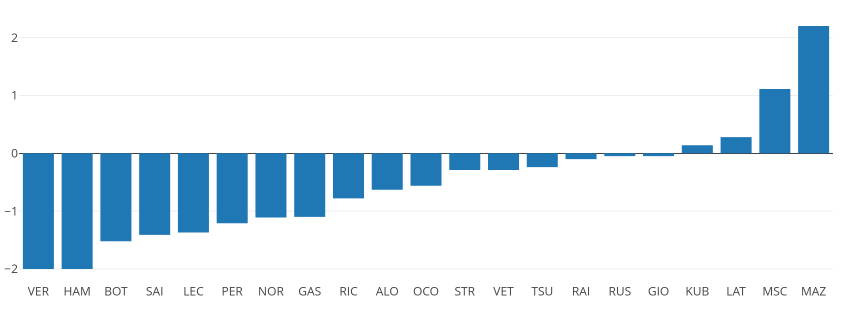
\includegraphics[scale=0.4]{results/seasonanalysis/positionDelta.png}
	\centering
	\caption{Diferencia entre posición de salida y al final en la temporada 2021 por piloto}
	\label{fig:positionDelta}
	\centering
\end{figure}


% Nuevo capítulo
\chapter{Experimentos / Validación}
\label{sec:expVal}
\newpage


\section{Respuestas a las consultas}

En este apartado se proporcionarán las respuestas obtenidas a las consultas descritas en los apartados anteriores. Veremos tanto respuestas obtenidas directamente con Spark en formato de texto como gráficas resultantes de la utilización de la librería Plotly. Nos vamos a centrar en los resultados de la query \quotes{Análisis de temporada por piloto}. El resto de resultados se podrán consultar en el apéndice \ref{sec:apendice2}

A lo largo de esta sección van a aparecer en numerosas ocasiones los códigos de piloto en lugar de sus nombres completos. Esto es por mantener las figuras con un tamaño. A continuación se proporciona una leyenda que establece una correspondencia entre código de piloto y su nombre completo:

\begin{figure}[H]
	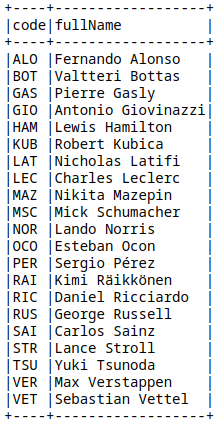
\includegraphics[scale=0.4]{leyendapilotos.png}
	\centering
	\caption{Leyenda de pilotos}
	\label{fig:leyendapilotos}
	\centering
\end{figure}


\subsection{Análisis de temporada por piloto}

En esta query se pretendía realizar un análisis sencillo de cierta temporada poniendo el foco en los pilotos. En concreto, buscábamos calcular las siguientes métricas:

\begin{compactitem}
	\item Puntos conseguidos en el campeonato.
	\item Media de puntos.
	\item Porcentaje de puntos respecto al piloto que más obtuvo.
	\item Total de podios.
	\item Porcentaje de carreras acabadas en podio.
	\item Diferencia media entre la posición de salida y la obtenida al cruzar la meta.
	\item Media de posiciones perdidas.
	\item Media de posiciones ganadas.
	\item Total de posiciones ganadas y perdidas.
	\item Vueltas lideradas.
	\item Porcentaje de vueltas lideradas.
\end{compactitem}

En este caso, como en el \texttt{DataFrame} final tenemos muchas métricas, no nos interesa mostrarlos en forma de texto como en el caso anterior, sino que para facilitar el análisis, sería más conveniente mostrar las métricas de forma gráfica.

A continuación se presenta un gráfico en el que podemos ver en el eje horizontal los distintos pilotos y en el vertical el valor de su \texttt{positionDelta}. El código utilizado para obtenerlo se ha descrito en el apartado \ref{plotly}.

\begin{figure}[H]
	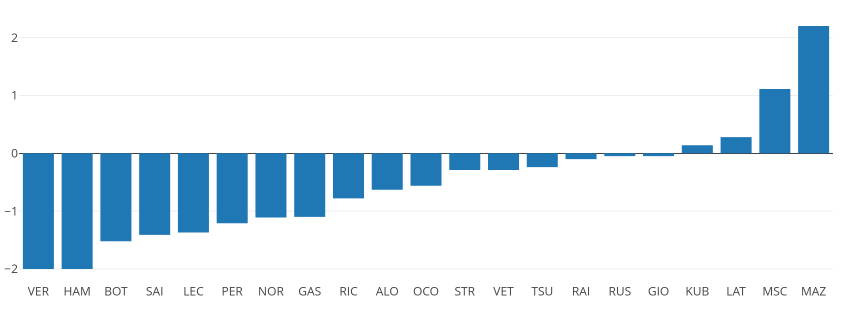
\includegraphics[scale=0.35]{results/seasonanalysis/positionDelta.png}
	\centering
	\caption{Diferencia entre posición de salida y al final en la temporada 2021 por piloto}
	\label{fig:positionDelta2}
	\centering
\end{figure}

Podemos llegar a la conclusión de que, cuanto más adelante clasifiques, más posiciones es probable que pierdas. Probablemente esto sea por que hay menos gente para adelantar, mientras que si clasificas al final de la parrilla será más fácil hacer adelantamientos y más difícil ser adelantado al tener menos gente detrás.

Otra métrica que resulta interesante es la media de posiciones perdidas, que será en parte análoga a la recién mostrada. Los resultados son los siguientes:

\begin{figure}[H]
	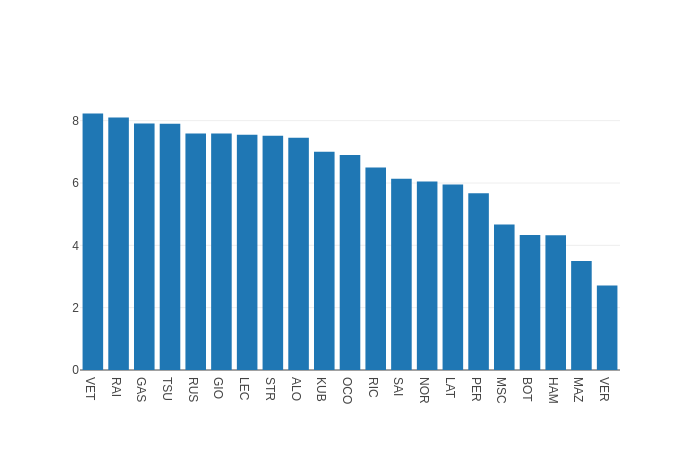
\includegraphics[scale=0.4]{results/seasonanalysis/avgpositionslost2021.png}
	\centering
	\caption{Media de posiciones perdidas en la temporada 2021 por piloto}
	\label{fig:avgPosLost2021}
	\centering
\end{figure}

Podemos llegar a la conclusión de que, de media, pierden menos posiciones los que están más al frente y al final de la parrilla. También podemos llegar a la conclusión de que esta temporada fue una con mucha diferencia entre el grupo de constructores que competían por el título, el grupo medio y el grupo más bajo, ya que vemos que los pilotos que de media acabaron al frente y al final solían perder menos posiciones que los pilotos del grupo medio.

La posición media en la que terminaron los pilotos en esta temporada la podemos ver a continuación:

\begin{figure}[H]
	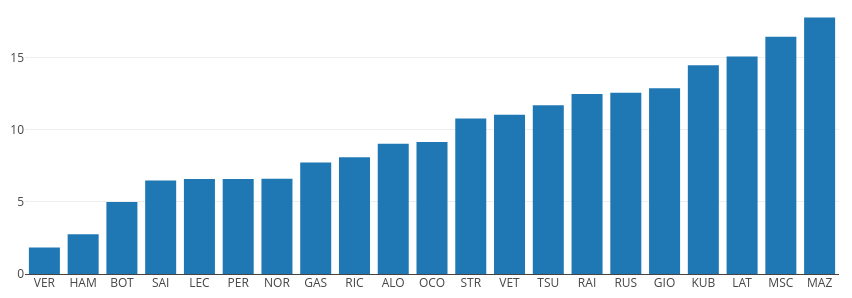
\includegraphics[scale=0.4]{results/seasonanalysis/avgfinishpos2021.png}
	\centering
	\caption{Media de posiciones finales en la temporada 2021 por piloto}
	\label{fig:avgFinPos2021}
	\centering
\end{figure}

Otra métrica interesante es el porcentaje de vueltas lideradas a lo largo de la temporada. Podemos obtener el siguiente gráfico:

\begin{figure}[H]
	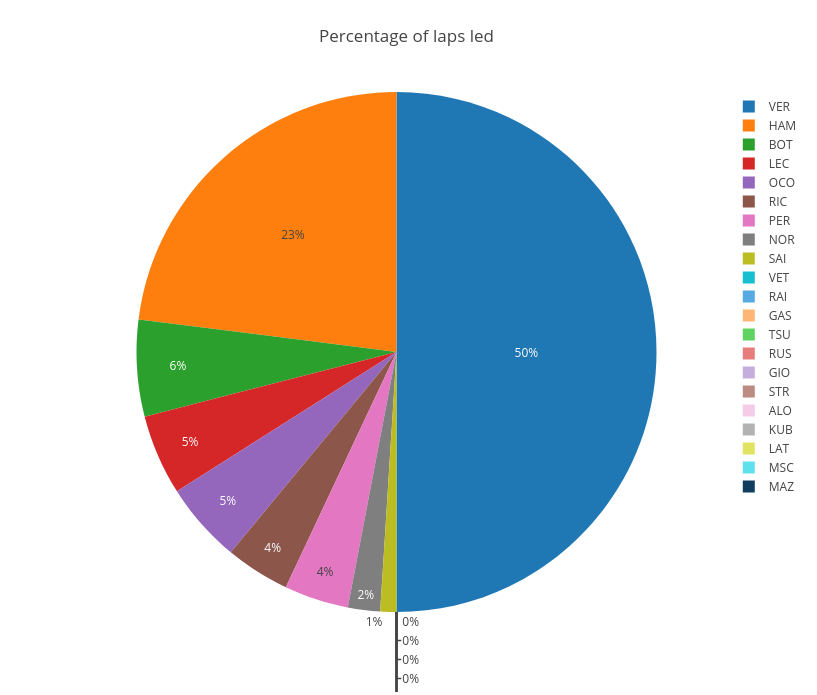
\includegraphics[scale=0.35]{results/seasonanalysis/percLapsLed2021.png}
	\centering
	\caption{Porcentaje de vueltas lideradas en la temporada 2021 por piloto}
	\label{fig:percLapsLed2021}
	\centering
\end{figure}

Se observa que la mitad de las vueltas han sido lideradas por Max Verstappen, mientras que su competidor por el título, Lewis Hamilton, lideró un 23\% de las vueltas. Aquí podemos ver de nuevo representada la diferencia de los dos contendientes al título respecto al resto de pilotos. Sin embargo, también podemos concluir que no es necesario liderar la mayoría de vueltas para competir por el título, ya que a pesar de lo que se muestra en esta métrica, tanto Max como Lewis llegaron igualados en puntos a la última carrera de la temporada. 

Podemos achacar que Max no dominase la temporada en puntos a que quizá a Lewis le costase adelantarle, ya que, como vimos antes, de media terminó por detrás de su contrincante. Se podría explicar también si Max hubiese tenido más problemas de fiabilidad y, a pesar de haber liderado la carrera, hubiese tenido que abandonar más carreras que Lewis.



\section{Comparativas de rendimiento}

En este apartado se va a realizar una comparativa de rendimiento entre ambas API. Para ello se van a comparar distintas métricas obtenidas de la Spark UI. A grandes rasgos se van a comparar el número de Jobs, Stages y Tasks de cada proceso, así como su Task Time, el total leído de disco y el total leído y escrito en \textit{shuffles}.

Además, se va a comparar el rendimiento de Spark al usar ficheros de entrada en formato CSV, parquet sin particionar y parquet particionado.

A la hora de hacer comparativas de este estilo, es importante igualar lo máximo posible las condiciones y el entorno del que dependen las mediciones. En nuestro caso, es importante que ambas sesiones de Spark cuenten con los mismos recursos y que el código sea lo más parecido posible, sin ninguna optimización de por medio. Por ejemplo, si para una de las API usamos una UDF, pero en la otra no es necesario porque existen mecanismos para evitarla, entonces debemos en ambos casos usar la UDF.

Lo primero que necesitamos para ello es crear un objeto \texttt{SparkSession}. Esto se hace de la siguiente manera:

\begin{lstlisting}
val spark: SparkSession = SparkSession
	.builder()
	.config("spark.sql.shuffle.partitions", 4)
	.master("local[4]")
	.getOrCreate()
\end{lstlisting}

En nuestro caso con estas opciones es suficiente, ya que estamos dedicando 4 núcleos de nuestra máquina local y 4 particiones de shuffle para las tareas que vayamos a realizar. Sin embargo, existen otras opciones que podríamos añadir si fuese necesario, como un nombre para la aplicación con \texttt{.appName("Nombre")}. 

De esta manera, si quisiéramos configurar algún parámetro, lo haríamos añadiendo más modificaciones tal que: 

\begin{lstlisting}
val spark: SparkSession = SparkSession
	.builder()
	.config("spark.some.config.option", "some-value")
	.config("spark.some.config.option", "some-value")
	...
	.master("local[N]")
	.getOrCreate()
\end{lstlisting}

Una vez tenemos el \texttt{SparkSession} creado correctamente, podemos usarlo para leer y escribir datos en distintos formatos, como CSV o Parquet. Además, nos permitirá crear \texttt{DataFrames} a partir distintos de tipos de datos, como Listas o Tuplas.

En los ejemplos anteriores hemos visto cómo se crearía el \texttt{SparkContext} para la API de Scala, pero en el caso de usar PySpark, lo crearíamos de la siguiente manera:

\begin{lstlisting}
spark = SparkSession.builder\
	.config("spark.sql.shuffle.partitions", 4)\
	.master("local[4]")\
	.getOrCreate()
\end{lstlisting}

Ya que nuestras queries son sobre conjuntos de datos pequeños, conviene reducir el número de particiones de shuffle, ya que por defecto hay 200. Spark está pensado para volúmenes grandes de datos, y es por eso que tiene un valor tan alto. El \textit{shuffle} es la manera que tiene Spark de redistribuir datos a los distintos ejecutores e incluso entre máquinas. Como en nuestro caso estamos en un entorno local con 4 cores no hacen falta tantas particiones, y se ha optado por usar solamente 4.

Los procesos en sí serán los mismos descritos en apartados anteriores y, en el caso de los que no se hayan descrito para un determinado lenguaje, se habrá obtenido utilizando las técnicas mencionadas en el apartado \ref{sec:migracion}. La única diferencia respecto a los descritos es que al final se ejecutará un \texttt{collect} sobre el \texttt{DataFrame} que contiene los resultados, lo cual hará que se ejecute el plan.


%\subsubsection{Recogida de datos}

Como se ha mencionado ya brevemente, se recogerán las distintas métricas de los procesos de la Spark UI. La Spark UI es un servicio web que se crea por cada proceso de Spark que está ejecutando en el sistema. Por defecto se abre en el puerto 4040 en el momento en el que tenemos el \texttt{SparkContext} creado, y nos proporciona información sobre el propio proceso: número de etapas, tareas, etc.

En nuestro caso vamos a recolectar la siguiente información de cada proceso: trabajos completados, etapas completadas y saltadas, total de tareas completadas, tiempo de tarea, tamaño de la entrada y tamaños de datos leídos y escritos en operaciones de \textit{shuffle}. Esta información la recogeremos de las pestañas \quotes{Jobs}, \quotes{Tasks} y \quotes{Executors}.

\subsubsection{Comparativa entre APIs}

Explicado todo esto la comparativa queda tal que:

\begin{figure}[H]
	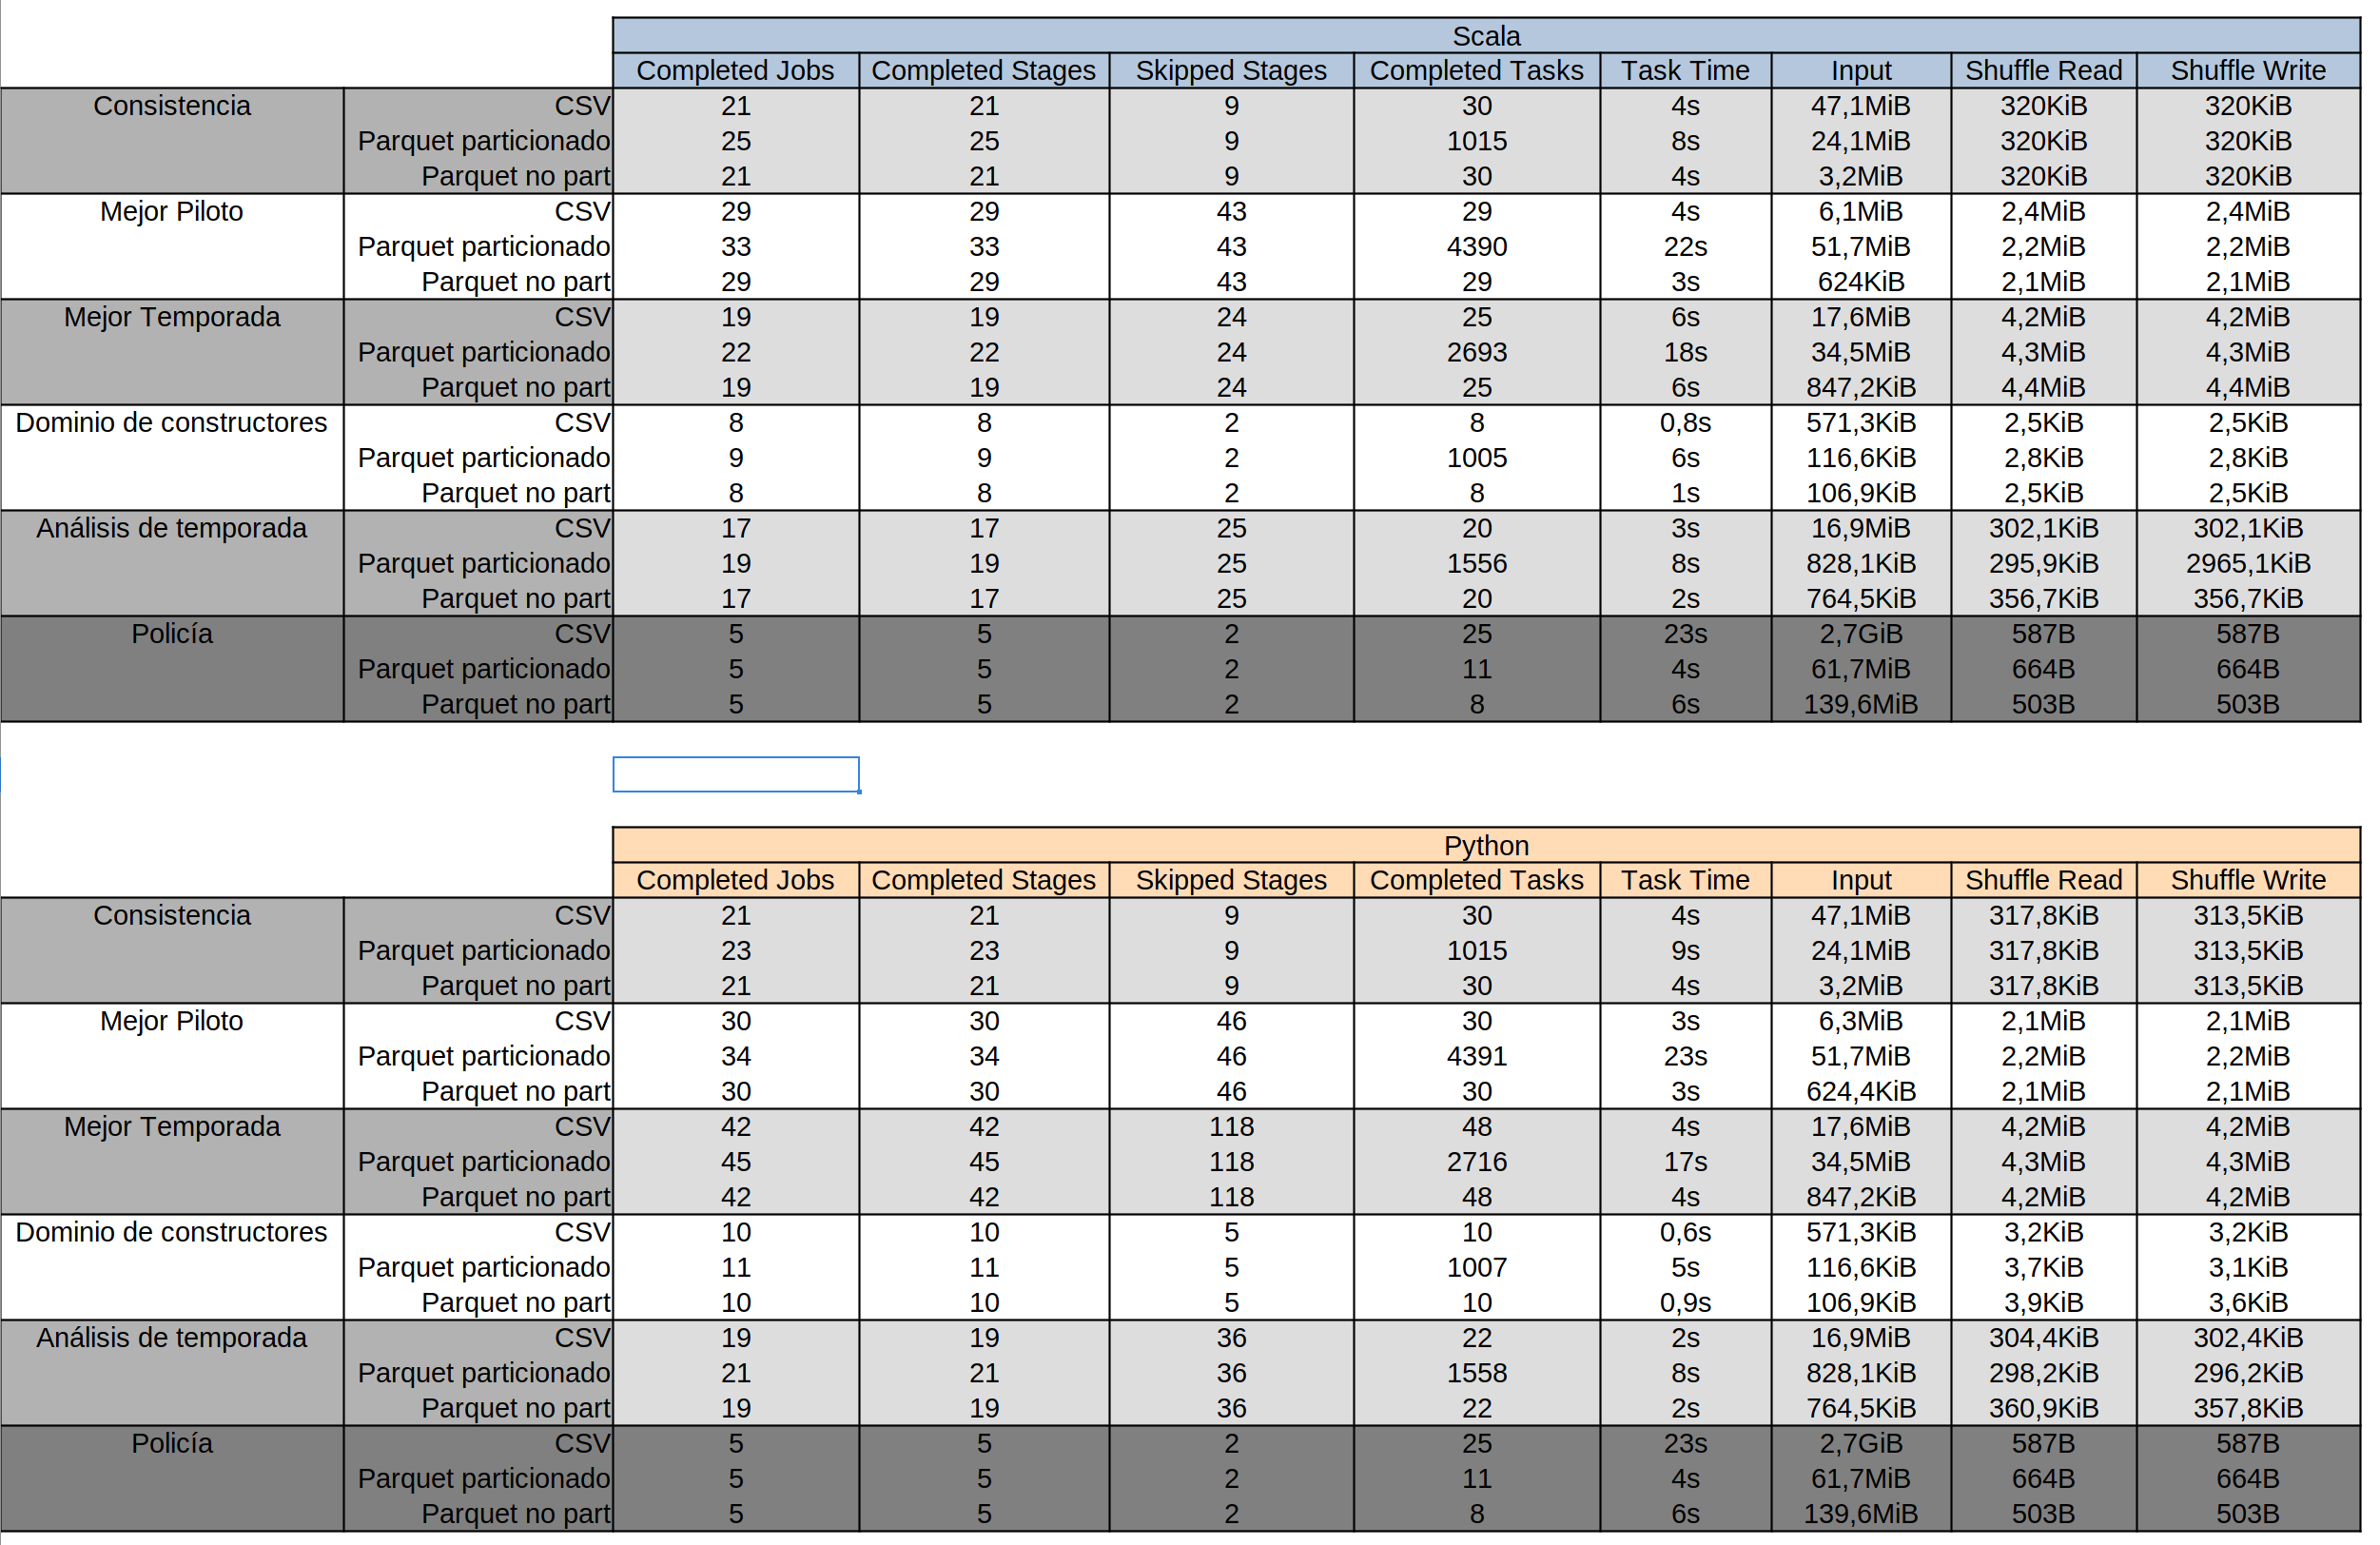
\includegraphics[scale=0.29]{comparativacompleta.png}
	\centering
	\caption{Comparativa entre APIs}
	\label{fig:completecomparison}
	\centering
\end{figure}

Como los resultados son bastante similares para todas las queries, vamos a centrarnos en una para explicar lo que ha sucedido. Más adelante explicaré el motivo de tener una query extra llamada \quotes{Policía}.

\begin{figure}[H]
	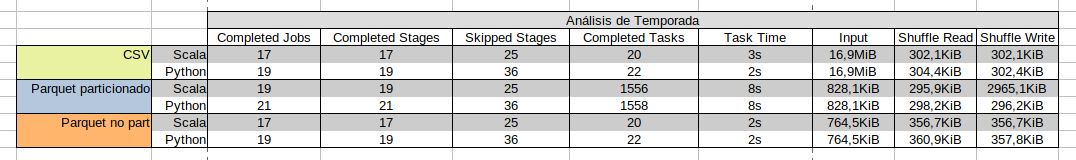
\includegraphics[scale=0.4]{analisistemporada.png}
	\centering
	\caption{Rendimiento de la query de análisis de temporada}
	\label{fig:companalisistemporada}
	\centering
\end{figure}

Podemos empezar centrándonos en los tiempos de tarea (Task Time). Se observa que los tiempos son muy bajos, de menos de 10 segundos para todas las mediciones. Esto puede significar varias cosas: que la máquina sobre la que se ejecutan las queries es demasiado potente o que el proceso dura muy poco, ya sea porque hace pocas operaciones o porque el conjunto de datos es muy pequeño. También podemos observar que la diferencia entre los tiempos de ejecución de ambas API es muy pequeña, siendo a veces inexistente.

Si miramos la parte del uso de memoria, podemos ver que de nuevo la diferencia entre API es prácticamente nula, a veces en el orden de Kibibytes. La diferencia más grande que podemos apreciar es a nivel de Trabajos, Etapas y Tareas, pero de nuevo la diferencia es muy baja. Esto se hace más evidente si nos fijamos en todas las queries en conjunto, donde el hecho de que la API de Scala genere menos Trabajos, Etapas y Tareas es algo constante salvo en la última query, y quizá podríamos llegar a la conclusión de que la API de Scala gestiona mejor esta parte del proceso, mientras que a veces su contraparte resulta ligeramente más eficiente en cuanto a tiempos de ejecución.

Se puede observar también que ocurre algo singular con la cantidad de trabajos y etapas completadas: normalmente el número es igual en ambos. Resulta curioso debido a que cada vez que se hace un \textit{shuffle} se crea una etapa nueva. Estos números tendrían sentido si no se produjera ningún \textit{shuffle}, sin embargo, podemos ver que sí se hace cierto \textit{shuffle} si nos fijamos en la cantidad de datos escritos y leídos en estas operaciones.

Para hallar la respuesta tendremos que fijarnos en otra de las métricas obtenidas: las etapas saltadas. Si nos fijamos en la query del Mejor Piloto con datos en formato Parquet particionado, veremos que tenemos 33 Jobs completados, 33 tareas completadas y 43 saltadas. La clave está en estas últimas: si Spark detecta que hay etapas que ya ha realizado, se las salta. Esto es posible debido a que el resultado de cada etapa completada se guarda en caché precisamente para evitar repetir operaciones. Podemos ver esto más detalladamente en las figuras \ref{fig:dagearly} y \ref{fig:daglate}.

\begin{figure}
	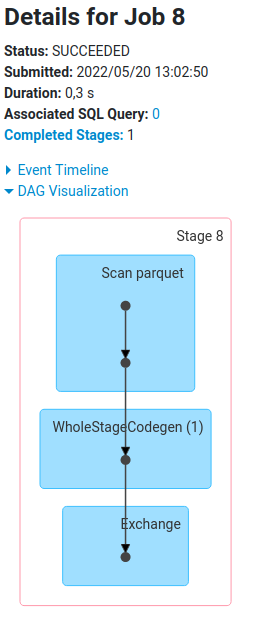
\includegraphics[scale=0.3]{dag_temprano.png}
	\centering
	\caption{Grafo de operaciones para un Job inicial}
	\label{fig:dagearly}
\end{figure}

Podemos ver cómo en el Job 8 se hacen las operaciones \quotes{Scan parquet}, \quotes{WholeStageCodegen} y \quotes{Exchange}, todas ellas en la etapa 8. La última de ellas es un \textit{shuffle}. Como comentamos antes, el Job acaba con uno de ellos.

\begin{figure}[H]
	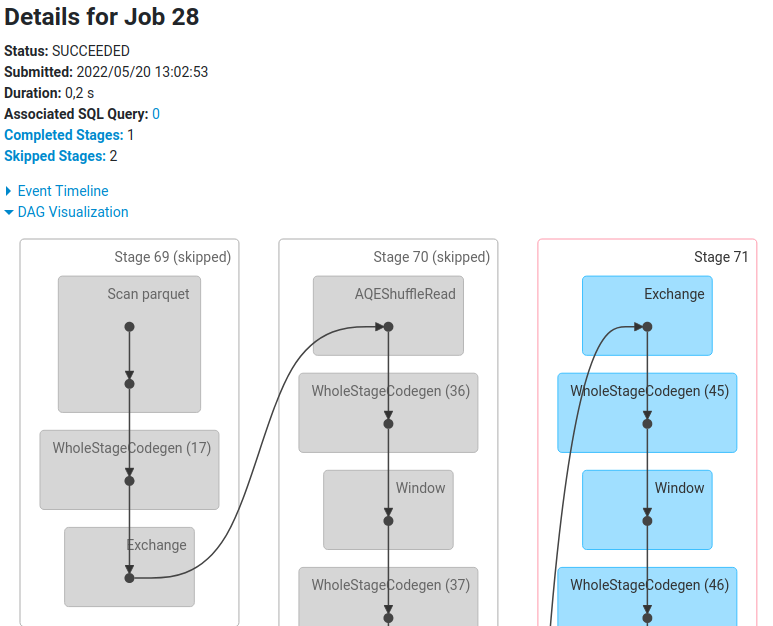
\includegraphics[scale=0.3]{dag_tardio.png}
	\centering
	\caption{Grafo de operaciones para un Job al final}
	\label{fig:daglate}
	\centering
\end{figure}

En las figuras vemos cómo en uno de los Jobs finales tenemos 3 etapas. En concreto es importante fijarse en la 69, que resulta ser la misma que la vista en la figura \ref{fig:dagearly}. Es por esto que el resultado ya está en caché y no es necesario volver a ejecutarla, lo cual provoca que se salte. Lo mismo pasa con la etapa 70, pero no con la 71, que es nueva y por tanto se ejecuta como sería natural.

Como he comentado antes brevemente, es posible que el conjunto de datos escogido para realizar las peticiones sea muy pequeño. Spark está pensado para manejar cantidades muy grandes de datos, en el orden de Gigabytes o más y, sin embargo, el conjunto de datos que escogí para realizar este trabajo es muy pequeño en comparación, en torno a los 20 Megabytes. Esto puede provocar que todo el procesamiento se haga en un solo núcleo y en una sola máquina, y esto no es para lo que fue diseñado.

Es por esto último que decidí hacer una query más con un conjunto de datos un poco más grande. Este consiste en un solo archivo en formato CSV de unos 1,4 Gigabytes sobre delitos cometidos en el estado de Nueva York. La query realiza una lectura de este archivo, un filtrado sencillo, una intersección y una escritura final, y busca obtener una correspondencia entre delitos cometidos en Manhattan y el Bronx en 2015 y los delitos cometidos en Queens y Brooklyn dos horas después.

El código de la query es la siguiente:

\begin{lstlisting}
val entiretable = spark.read.format("csv")
	.option("header", "true")
	.option("sep", ",")
	.load("../data/police/NYPD_Complaint_Data_Historic.csv")    
	.withColumn("CMPLNT_FR_DATETIME", to_timestamp(concat(col("CMPLNT_FR_DT"), lit(" "), col("CMPLNT_FR_TM")), "MM/dd/yyyy HH:mm:ss"))
	.withColumn("COMPLETE_LOC", concat(col("LOC_OF_OCCUR_DESC"), lit(" "), col("PREM_TYP_DESC")))
	
val crimesManh = entiretable
	.withColumn("CMPLNT_FR_DATETIME_2H_AFTER", col("CMPLNT_FR_DATETIME") + expr("INTERVAL 2 HOURS"))
	.where((col("BORO_NM") === "MANHATTAN" || col("BORO_NM") === "BRONX") && year(col("CMPLNT_FR_DATETIME")) === 2015)
	.withColumnRenamed("CMPLNT_FR_DATETIME", "CMPLNT_FR_DATETIME_MANH")
	.withColumnRenamed("CMPLNT_FR_DATETIME_2H_AFTER", "CMPLNT_FR_DATETIME_2H_AFTER_MANH")
	.withColumnRenamed("CMPLNT_FR_DT", "CMPLNT_FR_DT_MANH")
	.withColumnRenamed("CMPLNT_NUM", "CMPLNT_NUM_MANH")
	.select("CMPLNT_FR_DATETIME_MANH", "CMPLNT_FR_DATETIME_2H_AFTER_MANH", "CMPLNT_FR_DT_MANH", "CMPLNT_NUM_MANH")

val crimesQue = entiretable
	.withColumn("CMPLNT_FR_DATETIME_2H_AFTER_QUE", col("CMPLNT_FR_DATETIME") + expr("INTERVAL 2 HOURS"))
	.where((col("BORO_NM") === "QUEENS" || col("BORO_NM") === "BROOKLYN") && year(col("CMPLNT_FR_DATETIME")) === 2015)
	.withColumnRenamed("CMPLNT_FR_DATETIME", "CMPLNT_FR_DATETIME_QUE")
	.withColumnRenamed("CMPLNT_FR_DATETIME_2H_AFTER", "CMPLNT_FR_DATETIME_2H_AFTER_QUE")
	.withColumnRenamed("CMPLNT_FR_DT", "CMPLNT_FR_DT_QUE")
	.withColumnRenamed("CMPLNT_NUM", "CMPLNT_NUM_QUE")
	.select("CMPLNT_FR_DATETIME_QUE", "CMPLNT_FR_DATETIME_2H_AFTER_QUE", "CMPLNT_FR_DT_QUE", "CMPLNT_NUM_QUE")
	
val results = crimesManh
	.join(crimesQue, crimesManh.col("CMPLNT_FR_DT_MANH") === crimesQue.col("CMPLNT_FR_DT_QUE"), "fullouter")
	.where(col("CMPLNT_FR_DATETIME_QUE") <= col("CMPLNT_FR_DATETIME_2H_AFTER_MANH") &&
col("CMPLNT_FR_DATETIME_QUE") >= col("CMPLNT_FR_DATETIME_MANH"))
	.select("CMPLNT_FR_DATETIME_MANH", "CMPLNT_NUM_MANH", "CMPLNT_FR_DATETIME_QUE", "CMPLNT_NUM_QUE")
\end{lstlisting}

Simplemente ejecutando este proceso podemos ver una diferencia notable con respecto a las otras queries, y quizá, al ser más grande el conjunto de datos, sea más representativo de la realidad. Podemos ver las métricas recogidas sobre este proceso en la siguiente imagen:

\begin{figure}[H]
	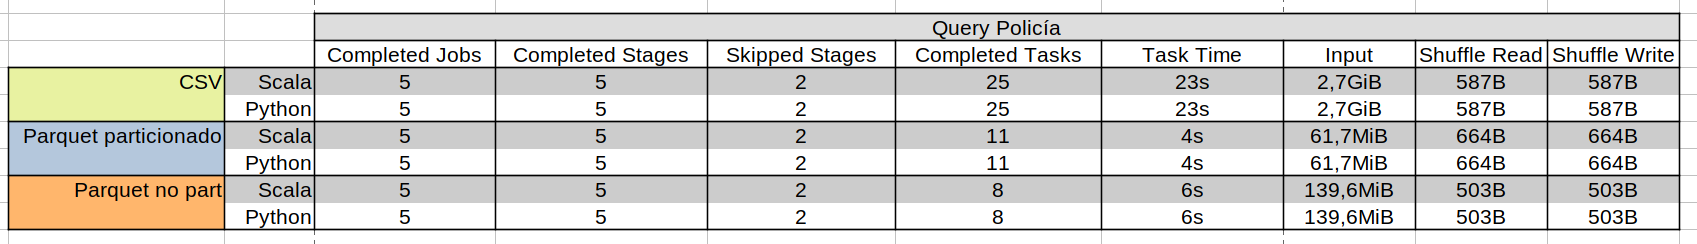
\includegraphics[scale=0.375]{comparativapolicia.png}
	\centering
	\caption{Rendimiento de la query extra}
	\label{fig:comppolicia}
	\centering
\end{figure}

Podemos deducir entonces que no existe una diferencia notable entre las API con los tamaños de datos que estamos manejando. Lo ideal sería realizar una query sobre un conjunto de datos que ronde las decenas o centenares de Gigabytes con el máximo paralelismo posible tanto a nivel de las propias máquinas (muchos núcleos y memoria dedicadas) como a nivel de nodos (varias máquinas conectadas entre sí).

Cabe destacar aquí que ambas API son interfaces de Apache Spark y, por lo tanto, dados dos \texttt{SparkContext} creados con los mismos parámetros y opciones que tengan asignados los mismos recursos, el rendimiento en teoría tendría que ser el mismo. Esto sería así salvo en un caso: que comparemos una API no nativa (como Python o R) a una nativa (Scala o Java) y utilicemos UDFs. En este caso al usar una API no nativa el modo en el que se aplica una UDF es diferente.


%\begin{filecontents}{\jobname.bib}
%	@online{sparkcore,
%		author = {QuantumBlack, a McKinsey company},
%		title  = {Spark UDF - Deep Insights in Performance},
%		date   = {2019-07-22},
%		url    = {https://medium.com/quantumblack/spark-udf-deep-insights-in-performance-f0a95a4d8c62}
%	}
%\end{filecontents}


Cuando usamos una API nativa, el código de la UDF compila directamente para la máquina virtual de Java (JVM a partir de ahora) y no es necesario llevar a cabo más operaciones: todo se queda en la JVM. Sin embargo, al usar una API no nativa, la UDF no puede compilar en la JVM y por lo tanto se lleva fuera de la misma para aplicar la función. Por ello es un proceso costoso en el que tenemos que pasaremos de tener los datos dentro de la JVM, para luego serializarlos fuera de ella, aplicarla función y deserializar para volver a tenerlos  dentro de la JVM. Como las UDF aplican funciones fila a fila cuanto más grande sea el conjunto de datos sobre el que se apliquen este tipo de funciones, mayor será el sobrecoste de usar una API no-nativa. Este proceso se denomina Serialización/Deserialización\footnote{\url{https://medium.com/quantumblack/spark-udf-deep-insights-in-performance-f0a95a4d8c62}}.

Una manera que tenemos para comprobar cómo afecta el paralelismo en los procesos de Spark resulta relativamente sencillo de implementar: podemos particionar la entrada y observar qué métricas nos arroja la Spark UI. Paralelizar la entrada en teoría debería permitir que Spark dedicase más tareas a la lectura y por lo tanto más recursos. En la siguiente sección veremos los detalles de cómo afecta esto al rendimiento.


\subsubsection{Comparativa entre tipos de fuentes de datos}

Hemos visto ya cómo afecta la propia API al rendimiento de las queries. Ahora vamos a intentar simular un paralelismo extra haciendo que en lugar de leer únicamente de un archivo lea la misma tabla, pero particionada de forma que tenga que, teóricamente, utilizar más tareas y recursos para leer.

Como he comentado brevemente antes, hay que tener especial cuidado a la hora de decidir qué columnas se usan para particionar. Es posible incluso que no nos merezca la pena particionar los datos. Vamos a ver un ejemplo de un \quotes{buen particionado} y uno \quotes{malo}.

Para ver el ejemplo del \quotes{mal} particionado, vamos a referir de nuevo a la figura \ref{fig:companalisistemporada}. Si en lugar de fijarnos en la comparativa entre APIs nos centramos en las diferencias entre formatos de entrada, podemos ver algo llamativo: al leer de un Parquet particionado se tarda más del doble que leyendo de un CSV y cuatro veces más que leyendo el Parquet sin particionar. 

En las queries sobre el conjunto de datos de la Fórmula 1 se decidió particionar la mayoría de tablas según el campo \texttt{raceId}, principalmente porque lo primero que se hace en muchas de ellas es filtrar por ese campo. Esto por norma general es buena práctica, ya que al particionar los datos según ese campo a la hora de llevar a cabo el procesado Spark tendrá un filtrado menos que hacer, pero las métricas obtenidas nos dicen otra cosa, ya que se esperaría que la query tardase menos y, lo más importante de todo, que leyese menos datos de disco.

Lo primero no se cumple y lo segundo se cumple en parte: lee mucho menos que al usar un CSV pero no se nota una diferencia notable entre particionar o no. Empecemos mirando el por qué de los tiempos de ejecución tan altos.

\begin{figure}[H]
	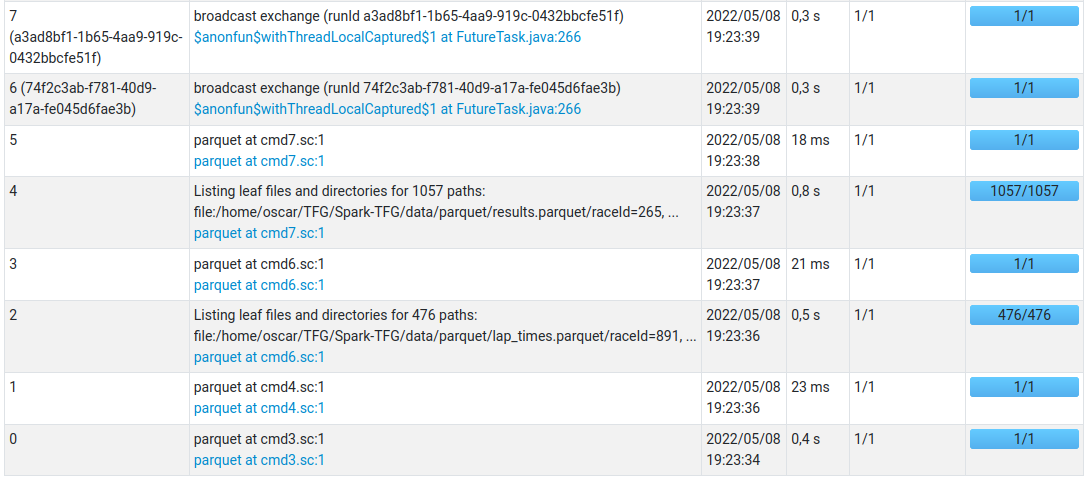
\includegraphics[scale=0.35]{tareaslecturaparquet.png}
	\centering
	\caption{Tareas al leer Parquet particionado}
	\label{fig:tareaslecturaparquet}
	\centering
\end{figure}

Como podemos observar en la figura anterior, que está obtenida de la pestaña "Jobs" de la Spark UI de un proceso que utiliza Parquet particionado, se pierde mucho tiempo listando el directorio de lectura. Además de eso, se crea una tarea para cada elemento del directorio en el que se encuentra la tabla (en este caso, 1057).

El otro problema que hemos visto es que no obtenemos una ganancia sustancial particionando si nos fijamos en la cantidad de datos leídos. Esto está relacionado con lo que acabamos de ver.

Como comentamos anteriormente, el conjunto de datos usado originalmente era demasiado pequeño para Spark, y por tanto llegamos a la conclusión de que no sacábamos todo el rendimiento que se podría sacar de esta API. Otro problema surgido de esto es que al particionar los ficheros Parquet creamos muchos archivos con muy pocos datos dentro. Por poner un ejemplo, la tabla \texttt{constructor$\_$standings} particionada por \texttt{raceId} tendrá N subcarpetas dependiendo del número de valores que tome el campo clave, y cada una de las particiones tendrá muy pocos datos en ella, en torno a 10 entradas de media, ya que es la cantidad de constructores que participan en una carrera.

Esto último saca a relucir otro problema: que al particionar una tabla tan pequeña es posible que los metadatos añadidos al utilizar Parquet como formato de entrada ocupen más que la propia información que contiene la tabla. La ya mencionada tabla \texttt{constructor$\_$standings} en formato CSV pesa en torno a 300KB. Usando Parquet sin particionar pesa en torno a 109KB y al particionar pesa exactamente 6MB.

\begin{figure}[H]
	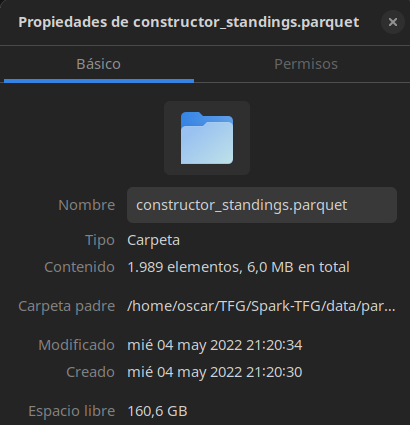
\includegraphics[scale=0.35]{pesoparquetparticionado.png}
	\centering
	\caption{Tamaño Parquet particionado}
	\label{fig:pesoparquetparticionado}
	\centering
\end{figure}

Por lo tanto, podemos llegar a la conclusión de que este superávit de tiempo de ejecución puede estar producido por el hecho de tener que leer tantos archivos. Si los archivos tuvieran más información y la query llevase a cabo un procesamiento más pesado lo más probable es que no se llegase a notar. Quizá leer un archivo grande no sea mucho más lento que leer uno pequeño y por tanto en el cómputo total fuese asumible. Sin embargo, al hacer operaciones a tan pequeña escala se notan mucho los tiempos gastados en listar directorios y leer particiones tan pequeñas.

Vamos a intentar mejorar el rendimiento de alguna query cambiando de modelo de particionado. En lugar de particionar gran parte de las tablas según \texttt{raceId}, vamos a particionar solamente \texttt{lap$\_$times}, y lo vamos a hacer según la columna \texttt{driverId}. El motivo de elegir esta combinación es el siguiente: la tabla en cuestión compone el 75\% del conjunto de datos (15MB de los 20MB que tenemos aproximadamente), y \texttt{driverId} tiene únicamente 135 entradas. Hay que mencionar que la tabla \texttt{drivers} tiene más de 800 entradas, pero como \texttt{lap$\_$times} sólo tiene datos a partir del año 1996, la cantidad de pilotos se reduce drásticamente.

Veamos ahora los resultados obtenidos y comparemos cara a cara con su contraparte \quotes{mal} particionada:

\begin{figure}[H]
	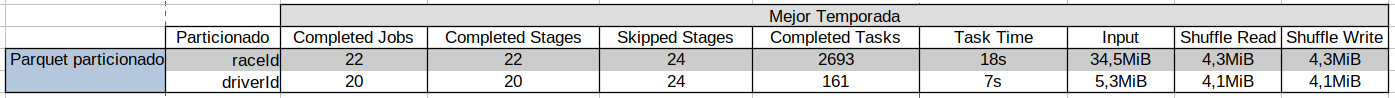
\includegraphics[scale=0.29]{comparativaparticionado.png}
	\centering
	\caption{Comparativa de particionado}
	\label{fig:comparativaparticionado}
	\centering
\end{figure}

Se puede observar una ganancia en todos los aspectos. La cantidad de Jobs es menor, hay menos etapas y, ante todo, la cantidad de tareas completadas se ha reducido drásticamente, al igual que el tiempo de ejecución, reducido a la mitad, y la cantidad de datos leídos, que es 6,5 veces menor.

Podemos llegar a la conclusión entonces de que el cómo particionemos los datos afecta directamente al rendimiento de nuestras peticiones.

Si centramos nuestra atención a la figura \ref{fig:comppolicia}, que utiliza un conjunto de datos mayor, veremos que leer de Parquet de nuevo siempre es mejor que leer un CSV, y por lo tanto concluimos que particionar si merece la pena.

Al tener un conjunto de datos más grande, leer de CSV resulta muy pesado ya que Spark tiene que leer línea a línea, columna por columna, inferir esquemas, etc. Al usar Parquet gran parte de este preprocesado se vuelve innecesario: el tipo de las columnas lo tenemos en los metadatos y solo necesitamos leer lo que realmente vamos a usar gracias a las optimizaciones de Spark. 

Tanto las ganancias en Task Time como en datos leídos de disco son muy grandes. Entre leer datos de un CSV y leer de un fichero Parquet particionado el Task Time se reduce aproximadamente a la mitad, y leemos 44 veces menos datos de disco.

Cabe destacar que esta tabla se ha particionado según un campo que toma una cantidad muy limitada de valores, y por lo tanto las particiones siguen siendo relativamente grandes, al contrario que en el particionado anterior.

De este apartado podemos, por tanto, sacar varias conclusiones rápidas: 

\begin{compactitem}
	\item No existe una diferencia real entre APIs, especialmente cuanto más grande es el conjunto de datos siempre que no usemos UDFs a menudo.
	\item Spark no funciona bien con pocos datos. Cuanto más, mejor.
	\item Cuanto más paralelismo, mejor.
	\item Para particionar correctamente una tabla es necesario conocer el contexto y no hacer las particiones demasiado pequeñas.
\end{compactitem}

En el siguiente capítulo elaboraré más estas conclusiones.


% Nuevo capítulo

\chapter{Conclusiones y trabajos futuros}
\newpage

En este trabajo hemos visto cómo se usa la API de Spark tanto en Scala como Python y hemos usado ambas para resolver cuestiones relacionadas con el dominio de la Fórmula 1. Tras obtener los resultados, estos han sido analizados con ayuda de la librería Plotly, que nos ayudó a generar gráficos sencillos.

También hemos visto cómo podemos migrar consultas de una API a otra, en este caso de Scala Spark a PySpark, ayudándonos de una serie de expresiones regulares para automatizar ligeramente la tarea.

Habiendo visto ya cómo se programa en ambas APIs, hemos pasado a analizar su rendimiento, y nos hemos encontrado con que el conjunto de datos que hemos usado para las consultas es demasiado pequeño y no utiliza todo el potencial que nos brinda Spark. Hemos visto también cómo el campo que utilicemos para particionar una tabla de entrada puede afectar al rendimiento.

Tras esto, hemos utilizado un conjunto de datos más grande y hemos visto que los datos obtenidos ya sí que resultaban más coherentes, aunque todavía no llegamos a utilizar todos los recursos de estas APIs.

Spark es una librería que permite acceder a fuentes de datos y realizar procesamiento tanto en paralelo en la misma máquina como de forma distribuida entre distintos nodos, y cuanto más grande sea la entrada y los datos que se manejan, más beneficio se saca a esta API. Quizá al tratarse de un conjunto de datos tan pequeño hubiese resultado más eficiente usar una librería como Pandas, que aunque no realice tantas optimizaciones como Spark resulta menos pesado y hubiese resultado en procesos más eficientes.

Sin embargo, para entornos en los que se manejan cantidades muy grandes de datos creo que Spark es la mejor opción, ya que las opciones que proporciona a la hora de paralelizar los procesos y distribuir el trabajo entre varios nodos resulta muy interesante si se tiene la infraestructura necesaria para darle uso.

Como hemos visto, la diferencia de rendimiento entre ambas API resulta prácticamente nula cuando se usan tamaños de entrada en el orden de Gigabytes, y sospecho que cuanto más grande sea el tamaño de entrada la diferencia será aún menor si es posible. Un punto clave en el que puede estar la diferencia entre ellas puede ser el uso de UDF ya que, aunque en las queries en las que las hemos usado no hemos notado diferencias notables, probablemente con una carga más grande de datos seguramente veamos que la balanza se inclina más a la API de Scala.

Como en rendimiento ambas API son idénticas en las comparaciones realizadas, entonces para llegar a una conclusión sobre cuál es mejor tenemos que comparar la experiencia de programar queries en Python y Scala. Esto roza el plano subjetivo, así que cada persona puede tener una opinión distinta al respecto, pero personalmente creo que la API de Scala es mejor en este aspecto.

En mi opinión la experiencia de programar queries de Spark en Scala resulta más natural que en su contraparte ya que la API fue diseñada inicialmente para ella, y por tanto tenía que cumplir con la filosofía del lenguaje. Si nos fijamos en otras librerías del estilo de Pandas, que fue diseñado con Python en mente, veremos que hacer queries resulta muy parecido a operar con listas o matrices. Veremos bucles y condiciones mientras que en Spark (y Scala) nos centramos en las transformaciones que debemos aplicar al conjunto de datos para obtener los resultados deseados al final.

En resumidas cuentas, programar queries usando PySpark puede resultar un choque de paradigmas de programación y quizá a alguien acostumbrado a programar en Python le resulte más intuitivo y natural usar una librería como Pandas.

Además, usando esta API en Scala disponemos de herramientas extra como las clases implícitas, que nos permiten extender la funcionalidad de clases como \texttt{DataFrame}, resultando así en un código más legible y limpio.

Hablando de esto último, en mi opinión el código queda mucho más limpio si usamos la API de Scala. Al migrar queries de ella a PySpark hemos visto que es un proceso en el que se añaden caracteres y, en general, ruido al código. Hacer el camino inverso por tanto será un proceso de limpieza de código.

Por estos motivos acababa usando Scala Spark en tareas secundarias. El código quedaba más limpio y me resultaba más rápido de desarrollar al no tener que preocuparme de añadir esos caracteres extra y centrándome en qué transformaciones quería hacer.

Por esto último, en mi opinión, la API de Scala es mejor que la de Python. Quizá no hayamos visto que se ahorre mucho tiempo de ejecución, pero definitivamente ahorramos en tiempo de desarrollo.

En general he disfrutado del desarrollo de este trabajo, a pesar de que ciertas etapas han podido resultar tediosas. En concreto las partes que más he disfrutado han sido la de la migración de queries y la comparativa final. La primera me ha permitido familiarizarme con la API de Python, ya que aunque el orden de este trabajo no lo refleje, se programaron todas las queries en Scala primero y una vez se vio que funcionaba y arrojaba los datos que se buscaban se migraron mediante el uso de las expresiones regulares. Esto también me permitió familiarizarme con ellas, ya que a pesar de haberlas visto a lo largo de la carrera nunca me fueron necesarias para el desarrollo de ninguna práctica, así que no pude afianzar las ideas.

Por otro lado la comparativa me permitió indagar un poco más en cómo funciona Spark por dentro, mirar cómo afectan factores que van más allá de la programación de queries al rendimiento: ya sea el particionado de los datos y su formato o la cantidad de recursos de los que se dispone.

La parte más tediosa fue la inicial. Familiarizarme con Spark, aprender los conceptos básicos de Scala o informarme sobre el dominio del el que iban a tratar las cuestiones planteadas como queries. También se me hizo complicado y largo el proceso de programación de las queries, pero principalmente achaco esto último a factores externos a la realzación del propio proyecto.

Finalmente, me gustaría comentar que he aprendido mucho con la realización de este proyecto y he adquirido conocimientos que seguro que más adelante me serán muy útiles en el ámbito profesional.

\section{Trabajos futuros}

A raíz de todo lo visto a lo largo de esta memoria quedan varios asuntos pendientes que se podrían desarrollar en trabajos futuros. Estos se describirán a continuación.

Respecto a la comparativa, queda pendiente comparar ambas API con un conjunto de datos más grande, idealmente en las decenas o cientos de Gigabytes y varios nodos que utilicen todo el potencial de Spark. Hemos visto que los resultados se estabilizan cuando aumentamos el tamaño de los datos de entrada. Por ello y por lo que ya hemos comentado anteriormente, lo justo sería realizar una comparativa parecida a la ya realizada pero con un contexto en el que Spark funcione de forma óptima y en un entorno lo más parecido posible a los que se tuvieron en mente a la hora de su diseño.

Por otro lado tendríamos automatizar la migración de queries mediante la utilización de las expresiones regulares diseñadas. Como ya comenté en el apartado dedicado a ello, quedan pendientes varias expresiones que quizá no sea posible implementar, pero sería relativamente sencillo programar un script de Bash que analice uno de Python y vaya aplicando las expresiones regulares ya vistas con sus correspondientes sustituciones usando \texttt{sed} y finalmente el archivo original quede sustituido por su homólogo de Scala.

%Como hay partes que requieren de intervención manual, quizá se podría detectarlas y hacer que en el script se ejecute un \textit{parser} que vaya comprobando carácter por carácter, formando \quotes{oraciones}, si se puede hacer algo con ellas. El ejemplo que se me viene a la cabeza es el de añadir paréntesis a cada condición individual de una condición compuesta: quizá con una expresión regular no podamos añadirlos de golpe, pero si analizamos secuencialmente y separamos cada condición podríamos añadirlas sin mucho problema de forma similar a cómo funciona una máquina de Turing.


Otra opción para automatizar estas migraciones sería buscar la forma de \quotes{importar} el Job de una instancia de Spark a otra. Esto puede ser posible porque, como ya hemos comentado, PySpark es un envoltorio sobre Spark, lo cual implica que los planes que genere una API deberían funcionar en otra. Sería una forma que requeriría más investigación por mi parte, pero proporcionaría una precisión perfecta al descartar el factor humano que siempre existe al realizar una migración manual.


%%%%%%%%%%%%%%%%%%%%%%%%%%%%%%% Bibliografía %%%%%%%%%%%%%%%%%%%%%%%%%%%%%%%

\phantomsection
\addcontentsline{toc}{chapter}{Bibliografía}

\footnotesize{
\bibliographystyle{hispa}
%\bibliographystyle{IEEEtran}
\bibliography{bibliografia}
}



% No expandir elementos para llenar toda la página
\raggedbottom
\afterpage{\blankpage}

\newpage




%%%%%%%%%%%%%%%%%%%%%%%%%%%%%%% Apéndices %%%%%%%%%%%%%%%%%%%%%%%%%%%%%%%

\appendix

\phantomsection
\addcontentsline{toc}{chapter}{Apéndices}

\mbox{}
\vfill
\begin{center}
\begin{Huge}
\textbf{Apéndices}
\end{Huge}
\end{center}
\vfill
\mbox{}
\thispagestyle{empty}

\newpage
\mbox{}
\thispagestyle{empty}
\newpage


% Primer apéndice
\chapter{Programación de queries}
\label{sec:apendice}

\section{Programación de queries en Scala Spark}

\label{extrascala}

\subsection{Análisis de temporada por piloto} \label{analisistemporada}

Esta query consiste en obtener una serie de métricas para cada piloto de una determinada temporada. Aunque no es un análisis muy en profundidad, se van a calcular varias métricas que nos ayudarán a arrojar un poco más de luz a la temporada que deseemos analizar. En nuestro caso será la temporada 2021 que, al resultar tan interesante de ver, suscitó preguntas que buscaremos resolver.

Primero necesitaremos información básica del piloto como su código o sus puntos en el campeonato. Tras esto veremos cómo de igualada ha estado la temporada calculando el porcentaje de puntos del resto de pilotos respecto al campeón. Veremos también cuántos puntos ha conseguido de media, su posición media al acabar la carrera y varias más como el porcentaje de vueltas lideradas o el total de adelantamientos. Entraremos más en detalle en la descripción de esta query.

El código es el siguiente:

\begin{lstlisting}
def queryAnalisisTemporada(season: Int, races: DataFrame, lap_times: DataFrame, results: DataFrame): DataFrame = {
	
	val driverWindow = Window.partitionBy("driverId")
	val seasonWindow = Window.partitionBy("year")
	val driverRaceWindow = Window.partitionBy("driverId", "raceId")
	val raceDriverLapWindow = Window.partitionBy("driverId", "raceId").orderBy("lap")
	
	val races_filtered = races
		.where(col("year") === season)
	
	val driverStats = lap_times	
		.withColumn("position", col("position").cast(IntegerType)) 
		.withColumn("lap", col("lap").cast(IntegerType)) 
		.join(races_filtered, "raceId")
	
		.withColumn("positionNextLap", lead(col("position"), 1).over(raceDriverLapWindow))
		.withColumn("positionsGainedLap", when(col("positionNextLap") < col("position") , abs(col("position") - col("positionNextLap"))).otherwise(0))
		.withColumn("positionsLostLap", when(col("positionNextLap") > col("position"), abs(col("position") - col("positionNextLap"))).otherwise(0))
		.withColumn("positionsGained", sum(col("positionsGainedLap")).over(driverRaceWindow))
		.withColumn("positionsLost", sum(col("positionsLostLap")).over(driverRaceWindow))
		.withColumn("lapLeader", when(col("position") === 1, 1).otherwise(0))
		.withColumn("lapsLed", sum(col("lapLeader")).over(driverWindow))
		.withColumn("totalLaps", sum(col("lapLeader")).over(seasonWindow))
		.withColumn("percLapsLed", round(col("lapsLed") / col("totalLaps"), 2))
		.select("raceId", "driverId", "positionsGained", "positionsLost", "lapsLed", "percLapsLed")
		.dropDuplicates()
	
	results
		.withColumn("position", col("position").cast(IntegerType))    
		.withColumn("grid", col("grid").cast(IntegerType))    
		.withColumn("points", col("points").cast(IntegerType))
	
		.join(races_filtered, "raceId")
		.join(driverStats, Seq("raceId", "driverId"), "left")
		.join(drivers, "driverId")
	
		.withColumn("podium", when(col("position") === 1 || col("position") === 2 ||col("position") === 3, lit(1)).otherwise(lit(0)))
		.withColumn("averagePoints", round(avg(col("points")).over(driverWindow), 2))
		.withColumn("maxAvgPoints", max(col("averagePoints")).over(seasonWindow))
	
		.select(
			col("code"),
			sum(col("points")).over(driverWindow).as("champPoints"),
			col("averagePoints"),
			round(col("averagePoints") / col("maxAvgPoints"),2).as("pointPercent"),
			sum(col("podium")).over(driverWindow).as("totalPodiums"),        
			round(avg(col("position")).over(driverWindow), 2).as("avgPosition"),
			round(sum(col("podium")).over(driverWindow) / count(col("podium")).over(driverWindow), 2).as("podiumPercent"),
			round(avg(col("position") - col("grid")).over(driverWindow), 2).as("positionDelta"),
			round(avg(col("positionsLost")).over(driverWindow), 2).as("avgPositionsLost"),
			round(avg(col("positionsGained")).over(driverWindow), 2).as("avgPositionsWon"),
			sum(col("positionsLost")).over(driverWindow).as("totalPositionsLost"),
			sum(col("positionsGained")).over(driverWindow).as("totalPositionsWon"),
			col("lapsLed"),
		col("percLapsLed")
		)
	
		.na.fill(0)
		.dropDuplicates(Seq("code"))
}
\end{lstlisting}



\subsubsection{Descripción detallada}

De nuevo, lo primero es obtener las distintas carreras que se han disputado en la temporada deseada. Para ello y como ya quedó explicado anteriormente, usaremos la tabla \texttt{races}, que filtraremos según la columna \texttt{year}.

Una vez obtenidas las carreras, necesitamos obtener información personal de los pilotos para más adelante sustituir su identificador numérico por el código de tres letras personal. Toda esta información la recibimos en el \texttt{DataFrame} \texttt{drivers}.

Tras esto, pasamos a crear las ventanas de datos que necesitaremos. En este caso, vamos a necesitar particionar los datos por piloto, por año, por piloto y carrera y de nuevo por piloto y carrera pero ordenando por vueltas. 

\begin{lstlisting}
val driverWindow = Window.partitionBy("driverId")
val seasonWindow = Window.partitionBy("year")
val driverRaceWindow = Window.partitionBy("driverId", "raceId")
val raceDriverLapWindow = driverRaceWindow.orderBy("lap")
\end{lstlisting}

Antes de continuar, necesitaremos obtener ciertos valores estadísticos relacionados con las posiciones del piloto a lo largo de la temporada. En concreto queremos obtener todas las posiciones ganadas y perdidas a lo largo de la carrera y, ya que usaríamos la misma tabla, el número y porcentaje de vueltas que ha liderado a lo largo de la temporada.

Para ello utilizaremos la tabla \texttt{lap$\_$times}, que filtraremos según las carreras de la temporada con el filtro que conseguimos antes. Para realizar estos cálculos, es importante además que las columnas \texttt{lap} y \texttt{position} sean enteros, ya que vamos a hacer comparaciones y sumatorios.

Todo esto lo podemos hacer de la siguiente manera:

\begin{lstlisting}
val driverStats = lap_times
	.withColumn("position", col("position").cast(IntegerType)) 
	.withColumn("lap", col("lap").cast(IntegerType)) 
	.join(races, "raceId")
\end{lstlisting}

Para calcular si un piloto ha ganado o ha perdido su posición en una vuelta, tenemos que saber cuál es su posición en la vuelta siguiente. Para ello podemos utilizar la función \texttt{lag} de la siguiente manera:

\begin{lstlisting}
	.withColumn("positionNextLap", lead(col("position"), 1).over(raceDriverLapWindow))
\end{lstlisting}


Con esto podemos calcular las vueltas ganadas o perdidas en cada vuelta de la siguiente manera:

\begin{lstlisting}
	.withColumn("positionsGainedLap", when(col("positionNextLap") < col("position") , abs(col("position") - col("positionNextLap"))).otherwise(0))
	.withColumn("positionsLostLap", when(col("positionNextLap") > col("position"), abs(col("position") - col("positionNextLap"))).otherwise(0))
\end{lstlisting}

De esta manera, aplicando la función \texttt{abs}, que nos devuelve el valor absoluto de la columna que se pasa como argumento, conseguimos dos de las métricas que buscábamos.

Para las otras dos métricas tendremos primero que conseguir las vueltas donde el piloto lideraba la carrera. Como tenemos información de todas las vueltas que han dado todos los pilotos en la temporada, obtener esta información no resulta complicado. Para esta query se ha realizado lo siguiente:

\begin{lstlisting}
	.withColumn("lapLeader", when(col("position") === 1, 1).otherwise(0))
\end{lstlisting}

Podemos entender esta columna a la que he llamado \texttt{lapLeader} de la siguiente manera: si el piloto ha liderado la vuelta, valdrá \texttt{1} y en caso contrario \texttt{0}. Esto resulta muy útil ya que podemos obtener el número de vueltas que un piloto ha liderado al hacer un sumatorio de todos los elementos de esta columna particionando por piloto, como se puede ver a continuación:

\begin{lstlisting}
	.withColumn("lapsLed", sum(col("lapLeader")).over(driverWindow))
\end{lstlisting}

Tras esto podemos obtener el porcentaje de vueltas que un piloto ha liderado dividiendo este valor recién calculado entre el total de vueltas dadas.

\begin{lstlisting}
	.withColumn("totalLaps", sum(col("lapLeader")).over(seasonWindow))
	.withColumn("percLapsLed", round(col("lapsLed") / col("totalLaps"), 2))
\end{lstlisting}

Finalmente, eliminamos duplicados y presentamos el \texttt{DataFrame} como consideremos oportuno. En este caso, necesitaré los cuatro valores calculados, el identificador de piloto y el de carrera.

\begin{lstlisting}
	.select("raceId", "driverId", "positionsGained", "positionsLost", "lapsLed", "percLapsLed")
	.dropDuplicates()
\end{lstlisting}

El siguiente paso es obtener la tabla final, y para ello partiremos de la tabla \texttt{results}. De nuevo necesitaremos convertir a entero ciertas columnas. En este caso \texttt{position}, \texttt{grid} y \texttt{points}.

Filtramos las carreras de la temporada en cuestión y ampliamos la información con la tabla \texttt{driverStats} que acabamos de obtener y \texttt{drivers}, esta última para convertir el id de piloto en su código de 3 caracteres. Todo esto lo hacemos de la siguiente manera:

\begin{lstlisting}
results
	.withColumn("position", col("position").cast(IntegerType))    
	.withColumn("grid", col("grid").cast(IntegerType))    
	.withColumn("points", col("points").cast(IntegerType))
	
	.join(races, "raceId")
	.join(driverStats, Seq("raceId", "driverId"), "left")
	.join(drivers, "driverId")  
\end{lstlisting}

Para esta query tendremos que calcular el número de puntos obtenidos por el piloto, la media de puntos, el porcentaje de puntos en relación al ganador del campeonato, el número total de podios, el porcentaje de veces que el piloto ha acabado en el podio, el diferencial entre la posición de salida y en la que termina, la media y el total de posiciones perdidas y ganadas y el número y porcentaje de vueltas lideradas.

Antes de nada tenemos que calcular 3 valores que servirán para más adelante calcular el resto de métricas. Estos son la media de puntos, la media de puntos más alta y si el piloto ha terminado en podio o no.

De forma similar a lo visto anteriormente, para ver si un piloto ha acabado en podio podemos crear una columna llamada \texttt{podium}, que valdrá \texttt{1} si el piloto acaba en las tres primeras posiciones y \texttt{0} en caso contrario.

\begin{lstlisting}
	.withColumn("podium", when(col("position") === 1 || col("position") === 2 ||col("position") === 3, lit(1)).otherwise(lit(0)))
\end{lstlisting}

La media de puntos es sencilla de calcular, y la media más alta se calcula sobre el valor anterior de la siguiente manera:

\begin{lstlisting}
	.withColumn("averagePoints", round(avg(col("points")).over(driverWindow), 2))
	.withColumn("maxAvgPoints", max(col("averagePoints")).over(seasonWindow))
\end{lstlisting}

Una vez obtenidos estos 3 valores podemos calcular el resto. En general todos son o bien sumatorios o medias sobre ventanas de datos concretas. Para presentar los datos de manera más accesible, se redondean a dos decimales usando la funciíon \texttt{round}.

Llegados a este punto me gustaría detenerme para explicar la función \texttt{select}. A simple vista parece sencilla si la usamos como lo haríamos en SQL o como hemos hecho hasta ahora, pero existe otra manera de usarla. Si nos vamos a la definición de la función en la documentación de Spark, veremos que le podemos pasar o bien varios String o varios objetos de tipo \texttt{Column}. Si utilizamos esta función de esta última manera, se puede obtener una cierta mejora en el plan de Spark y, por lo tanto, es recomendable utilizarla así.

En este caso, he decidido mostrar cómo finalizaríamos la query usando un \texttt{select} que recibe columnas en lugar de String. 

\begin{lstlisting}
.select(
	col("code"),
	sum(col("points")).over(driverWindow).as("champPoints"),
	col("averagePoints"),
	round(col("averagePoints") / col("maxAvgPoints"),2).as("pointPercent"),
	sum(col("podium")).over(driverWindow).as("totalPodiums"),
	round(sum(col("podium")).over(driverWindow) / count(col("podium")).over(driverWindow), 2).as("podiumPercent"),
	round(avg(col("position") - col("grid")).over(driverWindow), 2).as("positionDelta"),
	round(avg(col("positionsLost")).over(driverWindow), 2).as("avgPositionsLost"),
	round(avg(col("positionsGained")).over(driverWindow), 2).as("avgPositionsWon"),
	sum(col("positionsLost")).over(driverWindow).as("totalPositionsLost"),
	sum(col("positionsGained")).over(driverWindow).as("totalPositionsWon"),
	col("lapsLed"),
	col("percLapsLed")
)
\end{lstlisting}

Como se puede observar, podemos pasarle una columna directamente o una operación sobre ciertas columnas que devuelva un objeto de tipo \texttt{Column} a la que damos nombre con \texttt{as}.

Para calcular todas estas métricas se utiliza siempre una ventana de datos que particiona por piloto, y en los que no se particiona es porque ya existe solamente una entrada por piloto.

Como queda algún registro con valor \texttt{null}, nos convendría tratar de alguna manera estos casos, ya que se pretende representar todas estas métricas gráficamente. Para ello se utilizan las funciones presentes en el paquete \texttt{na}. Hay tres funciones que cubrirán la mayoría de casos de uso que necesitemos. Estas son: \texttt{fill}, \texttt{replace} y \texttt{drop}. Su función la indica el nombre: \texttt{fill} rellena los nulos con un literal que pasamos por parámetro, \texttt{replace} sustituye los nulos según se especifique y \texttt{drop} elimina las filas que contengan nulos, con la opción de especificar en qué columnas comprueba la existencia de estos valores.

Para la función \texttt{replace} he encontrado muy útil que puede recibir como parámetro un objeto de tipo \texttt{Map}, en el que la clave será el nombre de la columna y el valor será el valor que queramos que sustituya a los nulos. Un ejemplo podría ser el siguiente: dado un DataFrame en el que tenemos tres columnas llamadas \texttt{id}, \texttt{name} y \texttt{salary}, si utilizásemos la función \texttt{na.replace()} pasándole como parámetro \texttt{Map(\quotes{name} --> \quotes{Pedro}, \quotes{salary} --> 0)} significaría que en la columna \texttt{name} los nulos pasarán a valer "Pedro" y para la columna \texttt{salary}, los valores nulos valdrán cero.

En nuestro caso, como se ha observado que los nulos aparecen cuando el piloto no tiene ninguna vuelta que haya liderado y solo en ese caso, podemos utilizar \texttt{na.fill(0)} para solventar el problema.

Tras esto solo quedaría eliminar entradas duplicadas y ordenar según la métrica que queramos mostrar gráficamente. Todo esto lo hacemos de la siguiente manera:

\begin{lstlisting}
	.na.fill(0)
	.dropDuplicates(Seq("code"))
	.sort(col("avgPositionsLost").desc)  
\end{lstlisting}

\section{Programación de queries en PySpark}
\label{extrapython}

\subsection{Mejor piloto de la historia}

Para averiguar cuál es el mejor piloto de la historia, debemos fijarnos en varios aspectos del piloto, como sus logros individuales, sin comparar con nadie más a la hora de hacer el cálculo y sus logros relativos a los compañeros de equipo a lo largo de su carrera.

Esta cuestión siempre es motivo de discusión en la comunidad de seguidores de este deporte: cada uno tiene su opinión basada en factores más o menos objetivos. Por esto mismo vamos a tratar de ver cuáles han sido los mejores de todos los tiempos y vamos a intentar establecer una clasificación en base a un sencillo sistema de puntuaciones que vamos a establecer.

Este sistema de puntos va a consistir en lo siguiente: dado el caso de que un piloto sea el mejor en cierta métrica y el tercero en otra, se hará la media de estas dos y obtendrá un total de dos puntos. Como vamos a tener varias métricas, la media se hará de su posición en el \textit{ranking} de cada una de ellas. Finalmente se hará una clasificación nueva en base a esa media. El que un piloto tenga una puntuación menor que otro nos indicará que está por encima de él.

Como es un hecho que no todas las carreras profesionales duran lo mismo, se va a tratar de \quotes{relativizar} todo lo posible estas métricas, es decir, se van a obtener métricas como \quotes{porcentaje de temporadas con victorias} o \quotes{posibilidad de pole}. En resumen, la mayoría de métricas van a ser medias o sumatorios divididos por o bien el número de carreras en las que ha participado o el número de temporadas en las que ha competido.

En la descripción detallada de esta query veremos más concretamente qué métricas calculamos y cómo lo hacemos.

Al calcular tantas métricas, queda un código bastante extenso que se proporciona a continuación completo para que el lector se pueda situar a medida que vayamos explicando la query:

\begin{lstlisting}
def averageRank(cols):
	return sum(cols) / len(cols)

averageRank = F.udf(averageRank, T.DoubleType())

def queryAnalisisTemporada(races, drivers, drivers_constr_season, driver_standings, results):

	raceDriverLapWindow = Window.partitionBy("driverId", "raceId").orderBy("lap")
	driverWindow = Window.partitionBy("driverId")
	seasonWindow = Window.partitionBy("year")
	teammateWindow = Window.partitionBy("year", "constructorId")
	raceConstructorWindow = Window.partitionBy("raceId", "constructorId")
	seasonConstructorWindow = Window.partitionBy("year", "constructorId")
	driverSeasonWindow = Window.partitionBy("driverId", "year")

	races = races\
		.select("raceId", "year")

	drivers = drivers\
		.select(F.col("driverId"),
			F.concat(F.col("forename"), F.lit(" "), F.col("surname")).alias("fullName"))

	lastRaces = races\
		.withColumn("round", F.col("round").cast(T.IntegerType()))\
		.withColumn("max", F.max(F.col("round")).over(Window.partitionBy("year")))\
		.where(F.col("round") == F.col("max"))\
		.select("raceId", "year")

	driverDomination = driver_standings\
		.join(lastRaces, ["raceId"], "right")\
		.join(driverConstSeasonMap, ["driverId", "year"], "left")\
		.withColumn("teamPointsPerc", F.col("points") / F.sum(F.col("points")).over(teammateWindow))\
		.withColumn("bestOfTeam", F.max(F.col("teamPointsPerc")).over(teammateWindow))\
		.withColumn("dominatedTeammate", F.when(F.col("teamPointsPerc") == F.col("bestOfTeam"), 1).otherwise(0))\
		.withColumn("dominationPerc", F.round(F.sum(F.col("dominatedTeammate")).over(driverWindow) / F.count(F.col("year")).over(driverWindow) * 100, 2))\
		.select("year", "driverId", "dominatedTeammate", "dominationPerc")

	driverFilter = results\
		.withColumn("finished", F.when(F.col("statusId") == 1, 1).otherwise(0))\
		.withColumn("numberOfFinishes", F.sum(F.col("finished")).over(driverWindow))\
		.where(F.col("numberOfFinishes") < 5)\
		.select("driverId")\
		.distinct()

	teammateComparison = results\
		.join(driverFilter, ["driverId"], "leftanti")\
		.join(races, "raceId")\
		.withColumn("position", F.col("position").cast(T.IntegerType()))\
		.withColumn("grid", F.col("grid").cast(T.IntegerType()))\
		.na.fill({"position" : 100, "grid" : 100})\
		.withColumn("grid", F.when(F.col("grid") == 0, 100).otherwise(F.col("grid")))\
		.withColumn("topPos", F.min(F.col("position")).over(raceConstructorWindow))\
		.withColumn("constructorBestPos", F.when(F.col("topPos") == F.col("position"), 1).otherwise(0))\
		.withColumn("topPosPerc", F.sum(F.col("constructorBestPos")).over(driverSeasonWindow) / 
F.count(F.col("raceId")).over(driverSeasonWindow) * 100)\
		.withColumn("constTopPosPerc", F.max(F.col("topPosPerc")).over(seasonConstructorWindow))\
		.withColumn("driverDomConstPos", F.when(F.col("constTopPosPerc") == F.col("topPosPerc"), 1).otherwise(0))\
		.withColumn("topGrid", F.min(F.col("grid")).over(raceConstructorWindow))\
		.withColumn("constructorBestGridPos", F.when(F.col("topGrid") == F.col("grid"), 1).otherwise(0))\
		.withColumn("topGridPerc", F.sum(F.col("constructorBestGridPos")).over(driverSeasonWindow) / 
F.count(F.col("raceId")).over(driverSeasonWindow) * 100)\
		.withColumn("constTopGridPerc", F.max(F.col("topGridPerc")).over(seasonConstructorWindow))\
		.withColumn("driverDomConstGrid", F.when(F.col("constTopGridPerc") == F.col("topGridPerc"), 1).otherwise(0))\
		.dropDuplicates(["driverId", "year"])\
		.withColumn("avgTopPosPerc", F.avg(F.col("topPosPerc")).over(driverWindow))\
		.withColumn("avgTopGridPerc", F.avg(F.col("topGridPerc")).over(driverWindow))\
		.withColumn("avgPosDom", F.avg(F.col("driverDomConstPos")).over(driverWindow))\
		.withColumn("avgGridDom", F.avg(F.col("driverDomConstGrid")).over(driverWindow))\
		.dropDuplicates(["driverId"])\
		.select("driverId", "avgTopPosPerc", "avgTopGridPerc", "avgPosDom", "avgGridDom")

	return results\
		.join(driverFilter, ["driverId"], "leftanti")\
		.join(races, "raceId")\
		.withColumn("grid", F.col("grid").cast(T.IntegerType()))\
		.withColumn("position", F.col("position").cast(T.IntegerType()))\
		.withColumn("firstRowStart", F.when((F.col("grid") == 1)  | (F.col("grid") == 2), 1).otherwise(0))\
		.withColumn("firstRowChance", F.round(F.sum(F.col("firstRowStart")).over(driverWindow) / F.count(F.col("firstRowStart")).over(driverWindow), 4) * 100)\
		.join(driverDomination, ["driverId", "year"], "left")\
		.join(teammateComparison, ["driverId"], "left")\
		.withColumn("avgGridStart", F.round(F.avg(F.col("grid")).over(driverWindow), 2))\
		.withColumn("avgFinish", F.round(F.avg(F.col("position")).over(driverWindow), 2))\
		.withColumn("pole", F.when(F.col("grid") == 1, 1).otherwise(0))\
		.withColumn("totalPolePositions", F.sum(F.col("pole")).over(driverWindow))\
		.withColumn("poleChance", F.round(F.col("totalPolePositions") / F.count(F.col("pole")).over(driverWindow), 4) * 100)\
		.withColumn("polesPerSeason", F.sum(F.col("pole")).over(driverSeasonWindow))\
		.withColumn("poleChance", F.round(F.col("totalPolePositions") / F.count(F.col("raceId")).over(driverWindow) * 100, 2))\
		.withColumn("hasPoleThisSeason", F.when(F.col("polesPerSeason") > 0, 1).otherwise(0))\
		.withColumn("percSeasonsWithPole", F.round(F.sum(F.col("hasPoleThisSeason")).over(driverWindow) / F.count(F.col("year")).over(driverWindow), 4) * 100)\
		.withColumn("win", F.when(F.col("position") == 1, 1).otherwise(0))\
		.withColumn("totalVictories", F.sum(F.col("win")).over(driverWindow))\
		.withColumn("victoryChance", F.round(F.col("totalVictories") / F.count(F.col("win")).over(driverWindow), 4) * 100)\
		.withColumn("winsPerSeason", F.sum(F.col("win")).over(driverSeasonWindow))\
		.withColumn("hasWonThisSeason", F.when(F.col("winsPerSeason") > 0, 1).otherwise(0))\
		.withColumn("percSeasonsWithWins", F.round(F.sum(F.col("hasWonThisSeason")).over(driverWindow) / F.count(F.col("year")).over(driverWindow), 4) * 100)\
		.withColumn("podium", F.when((F.col("position") == 1) | (F.col("position") == 2) | (F.col("position") == 3), 1).otherwise(0))\
		.withColumn("podiumChance", F.round(F.sum(F.col("podium")).over(driverWindow) / F.count(F.col("podium")).over(driverWindow), 4) * 100)\
		.dropDuplicates(["driverId"])\
		.select("driverId", "firstRowChance", "avgGridStart", "avgFinish", 
"totalPolePositions", "poleChance", "percSeasonsWithPole", 
"percSeasonsWithWins", "podiumChance", "dominationPerc", 
"avgTopPosPerc", "avgTopGridPerc", "avgPosDom", "avgGridDom")\
		.withColumn("rankFRC", F.rank().over(Window.orderBy(F.col("firstRowChance").desc())))\
		.withColumn("rankAGS", F.rank().over(Window.orderBy(F.col("avgGridStart").asc())))\
		.withColumn("rankAF", F.rank().over(Window.orderBy(F.col("avgFinish").asc())))\
		.withColumn("rankTPP", F.rank().over(Window.orderBy(F.col("totalPolePositions").desc())))\
		.withColumn("rankPSWP", F.rank().over(Window.orderBy(F.col("percSeasonsWithPole").desc())))\
		.withColumn("rankPSWW", F.rank().over(Window.orderBy(F.col("percSeasonsWithWins").desc())))\
		.withColumn("rankPC", F.rank().over(Window.orderBy(F.col("podiumChance").desc())))\
		.withColumn("rankDom", F.rank().over(Window.orderBy(F.col("dominationPerc").desc())))\
		.withColumn("rankPoleC", F.rank().over(Window.orderBy(F.col("poleChance").desc())))\
		.withColumn("rankPosPerc", F.rank().over(Window.orderBy(F.col("avgTopPosPerc").desc())))\
		.withColumn("rankGridPerc", F.rank().over(Window.orderBy(F.col("avgTopGridPerc").desc())))\
		.withColumn("rankPosDom", F.rank().over(Window.orderBy(F.col("avgPosDom").desc())))\
		.withColumn("rankGridDom", F.rank().over(Window.orderBy(F.col("avgGridDom").desc())))\
		.withColumn("stats", averageRank(
			F.array(F.col("rankFRC"),
				F.col("rankAGS"),
				F.col("rankAF"),
				F.col("rankTPP"),
				F.col("rankPSWP"),
				F.col("rankPSWW"),
				F.col("rankPC"),
				F.col("rankDom"),
				F.col("rankPoleC"),
				F.col("rankPosPerc"),
				F.col("rankGridPerc"),
				F.col("rankPosDom"),
				F.col("rankGridDom")
			)
		))\
		.withColumn("rank", F.rank().over(Window.orderBy(F.col("stats").asc())))\
		.sort(F.col("rank").asc())\
		.join(driverInfo, "driverId")
\end{lstlisting}

\subsubsection{Descripción detallada}

El primer paso para programar esta query es construir varios \texttt{DataFrames} auxiliares. Necesitaremos una tabla que relacione la carrera con la temporada en que tuvo lugar,  otra que nos relacione el identificador de piloto con su nombre completo, una que nos proporcione información sobre qué carreras fueron las últimas de cada temporada y por último una que establezca una relación entre los pilotos que formaron un equipo en cada temporada.

Para obtener la primera de ellas se usará la tabla \texttt{races} y nos quedaremos con las columnas \texttt{raceId} y \texttt{year}. 

\begin{lstlisting}
races = races\
	.select("raceId", "year")
\end{lstlisting}

Para la segunda usaremos la tabla \texttt{drivers} y nos quedaremos con las columnas \texttt{driverId} y una concatenación de las columnas \texttt{forename} y \texttt{surname} que llamaremos \texttt{fullName}.

\begin{lstlisting}
driverInfo = drivers\
	.select(F.col("driverId"),
	F.concat(F.col("forename"), F.lit(" "), F.col("surname")).alias("fullName"))
\end{lstlisting}

También necesitamos obtener la última carrera de cada temporada. Para ello usamos de nuevo la tabla \texttt{races} y convertimos la columna \texttt{round} a tipo \texttt{IntegerType}. Acto seguido, utilizamos una ventana que particione los datos según la columna \texttt{year} para obtener el máximo de la \texttt{round}. Por último, nos quedamos con las entradas donde \texttt{round} sea igual al máximo obtenido. El código es el siguiente:

\begin{lstlisting}
lastRaces = races\
	.withColumn("round", F.col("round").cast(T.IntegerType()))\
	.withColumn("max", F.max(F.col("round")).over(Window.partitionBy("year")))\
	.where(F.col("round") == F.col("max"))\
	.select("raceId", "year")
\end{lstlisting}


Adicionalmente, en algún momento necesitaremos filtrar pilotos para eliminar outliers. En el caso de esta query, se ha concluido que estos serán aquellos pilotos que no hayan terminado cinco carreras o más. Para ello, usamos la tabla \texttt{results} y nos fijamos en la columna \texttt{statusId}. Si el valor es \texttt{1}, entonces quiere decir que el piloto ha pasado por meta. Para calcular el número de carreras que ha terminado, podemos crear una columna nueva que contenga un \texttt{1} si el \texttt{statusId} tiene ese valor y \texttt{0} en caso contrario.

\begin{lstlisting}
driverFilter = results\
	.withColumn("finished", F.when(F.col("statusId") == 1, 1).otherwise(0))\
\end{lstlisting}

Acto seguido podemos hacer un sumatorio de esta columna particionando por piloto y después filtrar los que no lleguen a cinco. Al poder tener varias entradas por piloto, usamos la función \texttt{distinct()} para deshacernos de estos valores repetidos.

\begin{lstlisting}
	.withColumn("numberOfFinishes", F.sum(F.col("finished")).over(driverWindow))\
	.where(F.col("numberOfFinishes") < 5)\
	.select("driverId")\
	.distinct()
\end{lstlisting}

Por último, como ya comentamos cómo obtener una relación entre pilotos, fabricante y temporada en la sección  \ref{drivconstseasontabexplanation}, no entraremos al detalle de cómo se obtiene y simplemente la usaremos según nos viene dada en los argumentos de la función.

También necesitaremos las siguientes ventanas de datos auxiliares:

\begin{lstlisting}
raceDriverLapWindow = Window.partitionBy("driverId", "raceId").orderBy("lap")
driverWindow = Window.partitionBy("driverId")
seasonWindow = Window.partitionBy("year")
teammateWindow = Window.partitionBy("year", "constructorId")
raceConstructorWindow = Window.partitionBy("raceId", "constructorId")
seasonConstructorWindow = Window.partitionBy("year", "constructorId")
driverSeasonWindow = Window.partitionBy("driverId", "year")
\end{lstlisting}


A continuación podemos pasar a la primera query, con la que trataremos de averiguar el porcentaje de temporadas en las que, a lo largo de su carrera, un ha terminado por delante de su compañero de equipo.


Para ello, primero usaremos la tabla \texttt{driver$\_$standings}, que interseccionaremos con \texttt{lastRaces} para quedarnos con la clasificación en la última carrera de cada temporada y con \texttt{drivers$\_$constr$\_$season} para completar con la información que nos proporciona dicha tabla.

\begin{lstlisting}
driverDomination = driver_standings\
	.join(lastRaces, ["raceId"], "right")\
	.join(drivers_constr_season, ["driverId", "year"], "left")\
\end{lstlisting}

El siguiente paso es averiguar el porcentaje de puntos que cada piloto ha obtenido para el equipo en cada temporada. Para ello dividiremos los puntos obtenidos por un piloto entre el total del equipo, calculado haciendo un sumatorio de los puntos según la ventana \texttt{teammateWindow}.

Para ver si un piloto ha dominado a su compañero de equipo en una temporada en concreto, podemos usar este último valor calculado y averiguar el máximo entre los integrantes del equipo. Cuando en una entrada de la tabla tengamos que un piloto iguala en puntos a este máximo, sabremos que ha sido el dominante en esa temporada.

\begin{lstlisting}
	.withColumn("teamPointsPerc", F.col("points") / F.sum(F.col("points")).over(teammateWindow))\
	.withColumn("bestOfTeam", F.max(F.col("teamPointsPerc")).over(teammateWindow))\
	.withColumn("dominatedTeammate", F.when(F.col("teamPointsPerc") == F.col("bestOfTeam"), 1).otherwise(0))\
\end{lstlisting}

Con este último cálculo podemos ver cuántas temporadas ha dominado cada piloto, pero es más útil para nosotros relativizarlo a la carrera de cada piloto. Por ejemplo, si un piloto compite cuatro años y domina tres de ellos, su total de temporadas dominadas será tres, mientras que el porcentaje de su carrera en la que ha dominado a su compañero de equipo es del 75\%. Esto nos es útil ya que el número de temporadas en las que un piloto compite en el deporte puede variar drásticamente, desde una sola temporada a veinte por poner alguna cifra.

Con esto en mente, podemos contar el número de temporadas en las que ha dominado y dividirlo entre el número de temporadas en las que ha competido, utilizando para ambos parámetros una ventana de datos que particione por piloto

\begin{lstlisting}
	.withColumn("dominationPerc", F.round(F.sum(F.col("dominatedTeammate")).over(driverWindow) / F.count(F.col("year")).over(driverWindow) * 100, 2))\
\end{lstlisting}

Calculada esta métrica, podemos pasar a calcular el resto. Para ello primero usamos la tabla \texttt{results} y filtramos los outliers intersecamos con la tabla \texttt{driverFilter}. Para llevar a cabo este filtrado, debemos hacer la intersección de tipo \texttt{leftanti}. También interseccionamos con la tabla \texttt{races} para obtener información sobre la temporada en la que se llevó a cabo cada carrera.

Como las columnas \texttt{position} y \texttt{grid} son de tipo \texttt{String}, debemos cambiarlas a tipo entero y tratar los nulos en ambos casos. Esto último es importante, ya que al ordenar estas columnas los nulos quedan por encima del resto. Estos nulos aparecen debido a que no todas las entradas de esta columna contienen números. En el caso de que un piloto no haya terminado la carrera aparecerá un \quotes{\texttt{$\backslash$N}}.

Para encargarnos de estos valores nulos, se puede usar la función \texttt{na.fill()}, que en este caso recibirá un diccionario cuya clave será un \texttt{String} que denote el nombre de la columna y el valor será el que queremos dar en caso de encontrar un nulo. Para este caso se ha decidido que los nulos se sustituyan por el valor \texttt{100}, ya que en ambos casos nunca ha habido una carrera con ese número de competidores, asegurando así que siempre aparecerá el último si quisiéramos ordenar de menor a mayor.

\begin{lstlisting}
teammateComparison = results\
	.join(driverFilter, ["driverId"], "leftanti")\
	.join(races, "raceId")\
	.withColumn("position", F.col("position").cast(T.IntegerType()))\
	.withColumn("grid", F.col("grid").cast(T.IntegerType()))\
	.na.fill({"position" : 100, "grid" : 100})\
\end{lstlisting}

Habiendo terminado con la preparación del \texttt{DataFrame}, podemos calcular las siguientes métricas: el porcentaje de carreras en las que un piloto ha acabado mejor que su compañero en la parrilla de salida y al acabar y el porcentaje total de temporadas en las que ha quedado mejor que el compañero de equipo igual, tanto en la parrilla de salida como al acabar. Para ello lo primero será averiguar cuándo un piloto ha acabado por delante de su compañero de equipo en una carrera. Esto lo conseguiremos sacando el mínimo valor de la columna \texttt{position} particionando sobre fabricante y carrera y comparando con la posición en la que ha terminado cada piloto.

\begin{lstlisting}
	.withColumn("topPos", F.min(F.col("position")).over(raceConstructorWindow))\
	.withColumn("constructorBestPos", F.when(F.col("topPos") == F.col("position"), 1).otherwise(0))\
\end{lstlisting}

Tras esto podemos calcular el porcentaje de carreras en las que cada piloto ha estado por delante de su compañero dividiendo la suma de la última columna entre el conteo de carreras en la temporada del piloto.

\begin{lstlisting}
	.withColumn("topPosPerc", F.sum(F.col("constructorBestPos")).over(driverSeasonWindow) / 
	F.count(F.col("raceId")).over(driverSeasonWindow) * 100)\
\end{lstlisting}

El siguiente paso será cuantificar este dominio calculando el porcentaje de carreras de la temporada en la que ha quedado por delante del resto del equipo. Para ello primero tenemos que averiguar carrera a carrera dentro del equipo quien tiene el \texttt{topPosPerc} más alto, y \quotes{marcar} cuando nuestro \texttt{topPosPerc} sea el más alto para luego ver el porcentaje de temporadas que ha dominado.

\begin{lstlisting}
	.withColumn("constTopPosPerc", F.max(F.col("topPosPerc")).over(seasonConstructorWindow))\
	.withColumn("driverDomConstPos", F.when(F.col("constTopPosPerc") == F.col("topPosPerc"), 1).otherwise(0))\
\end{lstlisting}

Con una serie de operaciones muy similares, podemos calcular lo mismo pero en lugar de tener en cuenta la posición en la que termina la carrera, la posición en la parrilla de salida:

\begin{lstlisting}
	.withColumn("topGrid", F.min(F.col("grid")).over(raceConstructorWindow))\
	.withColumn("constructorBestGridPos", F.when(F.col("topGrid") == F.col("grid"), 1).otherwise(0))\
	.withColumn("topGridPerc", F.sum(F.col("constructorBestGridPos")).over(driverSeasonWindow) / 
	F.count(F.col("raceId")).over(driverSeasonWindow) * 100)\
	.withColumn("constTopGridPerc", F.max(F.col("topGridPerc")).over(seasonConstructorWindow))\
	.withColumn("driverDomConstGrid", F.when(F.col("constTopGridPerc") == F.col("topGridPerc"), 1).otherwise(0))\
\end{lstlisting}

Como queremos quedarnos con una entrada por piloto y temporada, aplicamos un \texttt{dropDuplicates} a las columnas pertinentes.

\begin{lstlisting}
	.dropDuplicates(["driverId", "year"])\	
\end{lstlisting}

Para calcular las métricas finales, haremos la media de las columnas \texttt{avgTopDom} y \texttt{avgDom}. La media de la primera columna nos dará el porcentaje de veces que ha quedado por delante de un compañero a lo largo de la carrera, tanto para la posición de salida como la de finalizado y la media de la segunda nos dará el porcentaje de temporadas en las que ha dominado a su compañero de equipo.

\begin{lstlisting}
	.withColumn("avgTopPosPerc", F.avg(F.col("topPosPerc")).over(driverWindow))\
	.withColumn("avgTopGridPerc", F.avg(F.col("topGridPerc")).over(driverWindow))\
	.withColumn("avgPosDom", F.avg(F.col("driverDomConstPos")).over(driverWindow))\
	.withColumn("avgGridDom", F.avg(F.col("driverDomConstGrid")).over(driverWindow))\
\end{lstlisting}

Por último, como solo queremos una entrada por piloto, hacemos otro \texttt{dropDuplicates} y seleccionamos las columnas que queremos que queden en el DataFrame.

\begin{lstlisting}
	.dropDuplicates(["driverId"])\
	.select("driverId", "avgTopPosPerc", "avgTopGridPerc", "avgPosDom", "avgGridDom")
\end{lstlisting}

Sin embargo, estas no son las únicas métricas que queremos calcular. Estamos interesados también en las siguientes:

\begin{compactitem}
	\item Posibilidad de que empiece la carrera en primera fila.
	\item Posición media de salida.
	\item Posición media al acabar la carrera.
	\item Total de poles.
	\item Porcentaje de poles relativo al número de carreras en las que se ha participado.
	\item Porcentaje de temporadas en las que ha conseguido una pole.
	\item Porcentaje de temporadas en las que ha ganado una carrera.
	\item Porcentaje de podios relativo al número de carreras en las que se ha participado.
\end{compactitem}

Primero, como viene siendo habitual, preparamos el DataFrame para los cálculos. Usamos la tabla \texttt{results} e interseccionamos con los DataFrames \texttt{driverDomination} según las columnas \texttt{driverId} y \texttt{year} y \texttt{teammateComparison} según la columna \texttt{driverId}. En ambos casos hacemos una intersección de tipo left. También interseccionamos con \texttt{races} para añadir información sobre la temporada en la que se ha disputado cada carrera.

Por último hacemos la intersección con \texttt{driverFilter} tomando como referencia la columna \texttt{driverId}. Sin embargo, esta intersección se hará de tipo \quotes{leftanti}. Esto quiere decir que el DataFrame resultante contendrá todos los elementos que no estén en el que queremos interseccionar por la derecha.

Esta es una manera eficiente de hacer un filtro en Spark. Otra manera sería hacer un \texttt{collect()} de \texttt{driverFilter} y obtenerlo como una lista. Llegados a este punto, en lugar de hacer una intersección \quotes{leftanti}, haríamos algo como:

\begin{lstlisting}
	.where(~F.col('driverId').isin(lista))
\end{lstlisting}

Sin embargo, hacer un \texttt{collect()} en Spark resulta muy costoso y por ello se ha optado por la primera opción.

De nuevo tendremos que convertir a tipo entero las columnas \texttt{grid} y \texttt{position}. El código para preparar este DataFrame es el siguiente:

\begin{lstlisting}
results =  results\
	.join(driverFilter, ["driverId"], "leftanti")\
	.join(races, "raceId")\
	.join(driverDomination, ["driverId", "year"], "left")\
	.join(teammateComparison, ["driverId"], "left")\
	.withColumn("grid", F.col("grid").cast(T.IntegerType()))\
	.withColumn("position", F.col("position").cast(T.IntegerType()))\
\end{lstlisting}

Lo primero que podemos calcular es el porcentaje de salidas en primera fila. Para ello primero tendremos que definir una columna que valga \texttt{1} cuando estemos en primera o segunda posición y \texttt{0} en otro caso. Para calcular la métrica podemos hacer sumar la columna recién definida particionando por piloto.

\begin{lstlisting}
	.withColumn("firstRowStart", F.when((F.col("grid") == 1)  | (F.col("grid") == 2), 1).otherwise(0))\
	.withColumn("firstRowChance", F.round(F.sum(F.col("firstRowStart")).over(driverWindow) / F.count(F.col("firstRowStart")).over(driverWindow), 4) * 100)\
\end{lstlisting}

Lo siguiente que podemos calcular es la posición de salida y la posición al acabar media. Esto se puede hacer con las siguientes líneas de código:

\begin{lstlisting}
	.withColumn("avgGridStart", F.round(F.avg(F.col("grid")).over(driverWindow), 2))\
	.withColumn("avgFinish", F.round(F.avg(F.col("position")).over(driverWindow), 2))\
\end{lstlisting}

También podemos calcular el total de poles, el porcentaje de poles respecto a todas las carreras disputadas y el porcentaje de temporadas en las que ha conseguido una pole.

Para ello primero tenemos que diferenciar las poles, esto es, cuando el piloto sale primero al iniciar la carrera. Después podemos sumar todas las poles de forma global para la primera métrica y particionando por temporada también para continuar calculando las siguientes.

El porcentaje de poles respecto al número de carreras podemos obtenerlo dividiendo el total con el conteo de carreras en las que ha participado el piloto. Para calcular el porcentaje de temporadas con pole, primero debemos de nuevo definir en qué temporadas ha conseguido alguna y hacer una cuenta similar a la anterior. Sumando todas las temporadas en las que se ha conseguido y dividiendo entre el total de campeonatos disputados. El código es el siguiente:

\begin{lstlisting}
	.withColumn("pole", F.when(F.col("grid") == 1, 1).otherwise(0))\
	.withColumn("totalPolePositions", F.sum(F.col("pole")).over(driverWindow))\
	.withColumn("polesPerSeason", F.sum(F.col("pole")).over(driverSeasonWindow))\
	.withColumn("poleChance", F.round(F.col("totalPolePositions") / F.count(F.col("raceId")).over(driverWindow) * 100, 2))\
	.withColumn("hasPoleThisSeason", F.when(F.col("polesPerSeason") > 0, 1).otherwise(0))\
	.withColumn("percSeasonsWithPole", F.round(F.sum(F.col("hasPoleThisSeason")).over(driverWindow) / F.count(F.col("year")).over(driverWindow), 4) * 100)\
\end{lstlisting}

Querríamos también hallar estas mismas métricas, pero para victorias. Esto resulta muy similar, salvo que en lugar de usar la columna \texttt{grid}, se usa la columna \texttt{position}:

\begin{lstlisting}
	.withColumn("win", F.when(F.col("position") == 1, 1).otherwise(0))\
	.withColumn("totalVictories", F.sum(F.col("win")).over(driverWindow))\
	.withColumn("victoryChance", F.round(F.col("totalVictories") / F.count(F.col("win")).over(driverWindow), 4) * 100)\
	.withColumn("winsPerSeason", F.sum(F.col("win")).over(driverSeasonWindow))\
	.withColumn("hasWonThisSeason", F.when(F.col("winsPerSeason") > 0, 1).otherwise(0))\
	.withColumn("percSeasonsWithWins", F.round(F.sum(F.col("hasWonThisSeason")).over(driverWindow) / F.count(F.col("year")).over(driverWindow), 4) * 100)\
\end{lstlisting}

También nos interesaría calcular el porcentaje de carreras en las que se ha obtenido un podio. Para ello primero definimos cuándo se ha conseguido un podio, es decir, cuando se ha terminado primero, segundo o tercero. Después y de forma muy parecida a los cálculos anteriores, podemos hacer una suma de todos los podios y dividir por el número de carreras disputadas.

\begin{lstlisting}
	.withColumn("podium", F.when((F.col("position") == 1) | (F.col("position") == 2) | (F.col("position") == 3), 1).otherwise(0))\
	.withColumn("podiumChance", F.round(F.sum(F.col("podium")).over(driverWindow) / F.count(F.col("podium")).over(driverWindow), 4) * 100)\
\end{lstlisting}

Por último, eliminamos la duplicidad según la columna \texttt{driverId} y seleccionamos las columnas que queremos que continúen.

\begin{lstlisting}
	.dropDuplicates(["driverId"])\
	.select("driverId", "firstRowChance", "avgGridStart", "avgFinish", 
	"totalPolePositions", "poleChance", "percSeasonsWithPole", 
	"percSeasonsWithWins", "podiumChance", "dominationPerc", 
	"avgTopPosPerc", "avgTopGridPerc", "avgPosDom", "avgGridDom")
\end{lstlisting}

Para finalizar esta query, crearemos una clasificación para cada métrica que hemos calculado. Algunas de menor a mayor y otras al contrario, y aplicaremos la UDF que programamos en la query anterior para hacer la media estas clasificaciones.

\begin{lstlisting}
return results\
	.withColumn("rankFRC", F.rank().over(Window.orderBy(F.col("firstRowChance").desc())))\
	...
	.withColumn("rankGridDom", F.rank().over(Window.orderBy(F.col("avgGridDom").desc())))\
	.withColumn("stats", averageRank(
	F.array(F.col("rankFRC"),
	F.col("rankAGS"),
	...
	F.col("rankGridDom")
	)
	))\
\end{lstlisting}

Además, creamos una columna que clasifique la columna \texttt{stats} de menor a mayor y ordenamos el \texttt{DataFrame} y ya por último completamos la información del piloto, en este caso nombre y apellido, interseccionando con el \texttt{DataFrame} \texttt{driverInfo}.


\chapter{Resultados obtenidos}
\label{sec:apendice2}

\section{Piloto más consistente en un periodo concreto de tiempo}

Con esta query el objetivo era averiguar qué piloto ha sido el más consistente en un periodo de tiempo determinado, en este caso la temporada 2012. Como ya explicamos anteriormente, hemos definido \quotes{consistencia} como la diferencia entre la media de las vueltas rápidas del piloto y la media de todas las vueltas dadas en todos los grandes premios de ese periodo.

En este caso, el resultado final de la query nos proporciona directamente la respuesta que buscamos. Ordena según el parámetro de consistencia calculado de mayor a menor, y lo acompaña con el nombre y el apellido del piloto en cuestión.

A continuación se puede ver el resultado de la query para la temporada 2012:

\begin{figure}[H]
	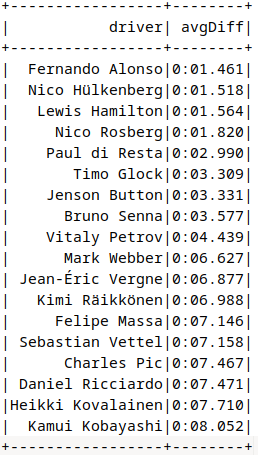
\includegraphics[scale=0.4]{results/consistency/2012consistency.png}
	\centering
	\caption{Correspondencia entre nombre del piloto y su código}
	\label{fig:2012consistency}
	\centering
\end{figure}

\section{Mejor piloto de la historia}

El objetivo de esta query era claro: intentar averiguar cuál ha sido el mejor piloto de la historia en base a varias métricas, que principalmente se dividen en dos grupos: comparativas con compañeros de equipo y estadísticas individuales. Por norma general se ha tratado de usar estadísticas relativas, es decir, en lugar de hacer un conteo de victorias, se ha hecho el conteo dividido por el número de carreras que en las que ha competido.

Como métricas individuales del piloto tenemos:
\begin{compactitem}
	\item Posibilidad de empezar la carrera en primera fila (primero o segundo).
	\item Media de posición en parrilla.
	\item Media de posición final.
	\item Posibilidad de hacer pole (clasificar primero).
	\item Porcentaje de temporadas con pole.
	\item Porcentaje de temporadas con al menos una victoria.
	\item Posibilidad de terminar la carrera en el podio.
	\item Total de poles.
\end{compactitem}

Cabe destacar que se ha tratado de encontrar métricas que sean imparciales. Por ejemplo, es probable que el piloto empiece su carrera en un equipo pequeño con un coche peor y que más adelante de el salto a otro más importante y con posibilidades de victorias y poles. Sin embargo, en mi opinión, un gran piloto debe poder llevar a cabo ciertos hitos en coches peores. Como ejemplos podríamos poner a Ayrton Senna en Mónaco 1984 o Fernando Alonso durante toda la temporada 2012. En ambos casos, la habilidad del piloto hizo posible conseguir resultados que de otra manera no hubiesen sido posibles. En resumen, si un piloto puede conseguir buenos resultados con coches no competitivos, entonces debe ser beneficiado.

También se ha buscado cierta justicia hacia el piloto, es decir, probablemente no siempre el mejor quede o clasifique primero. A veces la diferencia entre el primero y el segundo es mínima, y pienso que esto no debe penalizar. Por ello se han usado métricas como la posibilidad de acabar en podio o la de empezar en primera fila.

Como métricas que comparan pilotos del mismo equipo tenemos:
\begin{compactitem}
	\item Porcentaje de temporadas de su carrera en las que un piloto ha dominado a su compañero de equipo en puntos.
	\item Porcentaje de carreras en las que un piloto ha terminado por delante de su compañero de equipo.
	\item Porcentaje de carreras en las que un piloto ha clasificado por delante de su compañero de equipo.
	\item Porcentaje de temporadas en las que un piloto ha superado a su compañero de equipo en clasificación.
	\item Porcentaje de temporadas en las que un piloto ha superado a su compañero de equipo al acabar la carrera.
\end{compactitem}

Comparar pilotos de distintas épocas es complejo ya que el deporte en sí ha variado enormemente. Una de las mejores maneras de determinar si un piloto es bueno es comparar con su compañero de equipo en una determinada temporada, ya que en principio deberían tener el mismo coche. Si uno de ellos ha quedado siempre por delante del otro en clasificación, podemos asegurar que es más rápido.

Para obtener los resultados de esta query en forma de clasificación sencilla en la que se ordene a los pilotos de mejor a peor debemos buscar una forma de \quotes{unir} todas estas métricas para formar una sola. En este caso esto lo hemos hecho obteniendo un ranking de cada métrica y haciendo la media de las posiciones que ocupa cada piloto en los rankings de las métricas. Por ejemplo, si un piloto está en la primera posición en una métrica y tercero en otra, se obtiene como valor total la media de ambos, en este caso 1,5.

Si se aplica esto podemos obtener un resultado como el siguiente:

\begin{figure}[H]
	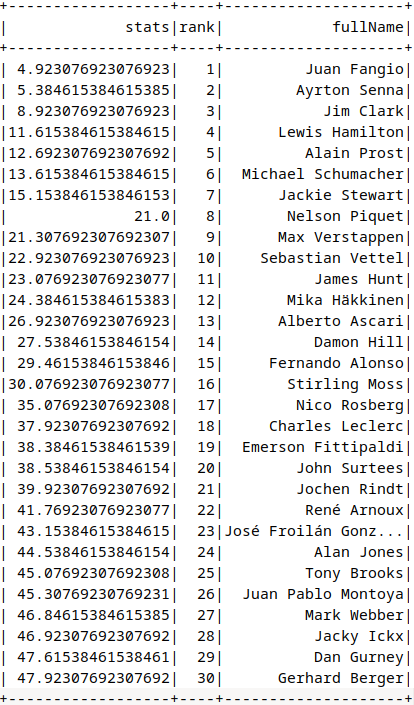
\includegraphics[scale=0.3]{results/bestdrivers/bestdrivers.png}
	\centering
	\caption{Ranking de mejores pilotos de la historia}
	\label{fig:bestDrivers}
	\centering
\end{figure}

Para contrastar el resultado podemos ver que todos estos pilotos de una manera u otra han pasado a la historia. En concreto las 6 primeras entradas independientemente del orden que cada uno pueda dar son considerados por muchos los mejores de todos los tiempos.

Además del resultado final podemos fijarnos también en los resultados de cada métrica, ya que en el DataFrame final se muestran tanto los resultados de cada una de ellas como el ranking de todas y el final. Por ilustrar esto, veamos el ranking de pilotos que han dominado a sus compañeros de equipo durante más temporadas a lo largo de su carrera:

\begin{figure}[H]
	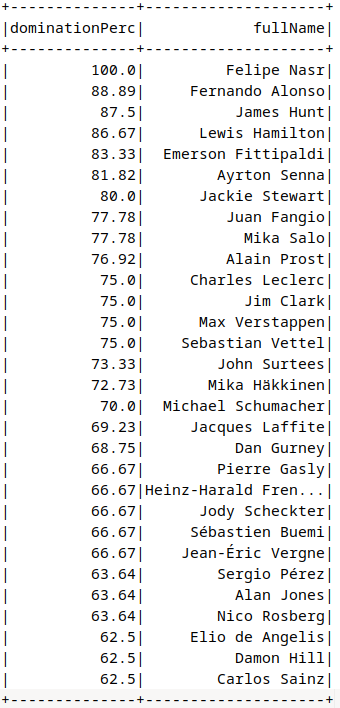
\includegraphics[scale=0.3]{results/bestdrivers/driverdomperc.png}
	\centering
	\caption{Ranking de pilotos más dominantes a lo largo de su carrera}
	\label{fig:dominationPerc}
	\centering
\end{figure}

Por clarificar el significado de esta métrica, \texttt{dominationPerc} nos indica el porcentaje de temporadas en las que un piloto ha dominado a su compañero de equipo.

Podemos observar que el primero de ellos es Felipe Nasr que, a pesar de tener una corta carrera de dos años, consiguió dominar a todos sus compañeros de equipo. Más notable es el caso de Fernando Alonso, que a pesar de su larga carrera en el deporte ha conseguido dominar al 88.89\% de sus compañeros de equipo. En las posiciones más altas de esta clasificación podemos ver a otros pilotos notables como James Hunt, Emerson Fittipaldi, Charles Leclerc o Lewis Hamilton.

Por poner varios ejemplos de métricas, podemos ver los pilotos con mejor posición de salida:

\begin{figure}[H]
	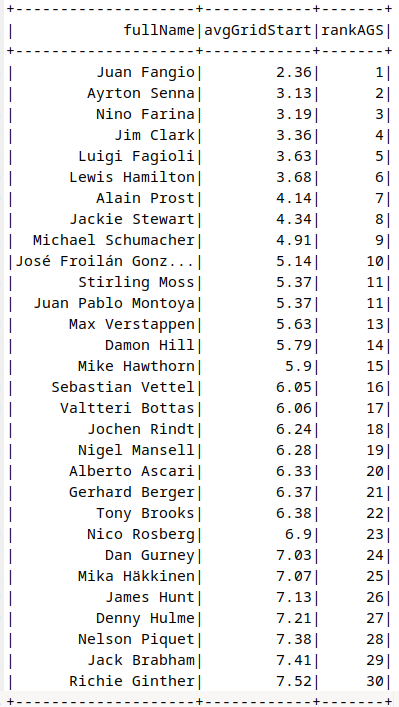
\includegraphics[scale=0.3]{results/bestdrivers/avggridstart.png}
	\centering
	\caption{Ranking de pilotos según su posición media de salida}
	\label{fig:avgGridStart}
	\centering
\end{figure}

O los pilotos con mayor porcentaje de clasificar primeros respecto al número de carreras en las que ha competido:

\begin{figure}[H]
	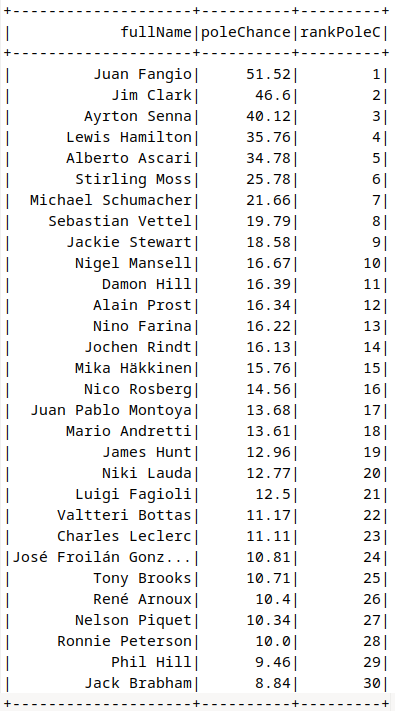
\includegraphics[scale=0.3]{results/bestdrivers/polechance.png}
	\centering
	\caption{Ranking de pilotos según su porcentaje de poles}
	\label{fig:poleChance}
	\centering
\end{figure}

\section{Mejor temporada}

Con esta query se buscaba averiguar cuál ha sido la mejor temporada de la historia. Para ello se han tenido en cuenta dos factores: el número de adelantamientos, el número de pilotos distintos que han liderado la clasificación general y el número de pilotos que han ganado al menos una carrera.

Como en la query anterior, debemos tener en cuenta varias métricas y se va a utilizar la misma metodología: hacer un ranking de cada una y hacer la media de todos los rankings. Tras aplicar esto, podemos ver que el resultado es el siguiente:

\begin{figure}[H]
	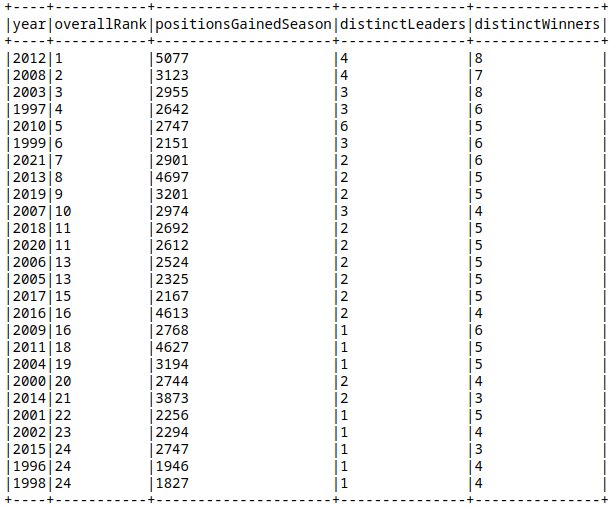
\includegraphics[scale=0.4]{results/bestseason/bestseasonstats.png}
	\centering
	\caption{Ranking de temporadas}
	\label{fig:bestseason}
	\centering
\end{figure}

Sin embargo, esta query tiene una limitación grande: no tenemos datos de las posiciones de los pilotos vuelta a vuelta de antes de 1996. En este caso, una de las métricas quedaría como nulo para las temporadas anteriores a la mencionada, y al hacer la media de los rankings el resultado no sería válido. Aun así podríamos interpretar esta query como "la mejor temporada en la historia reciente del deporte".

Esto nos afecta también a la hora de calcular el piloto más consistente de la temporada, ya que en ese caso no podemos obtener el tiempo por vuelta.

\section{Fabricante más dominante en un periodo concreto de tiempo}

En este caso se buscaba ver cuál ha sido el fabricante con más victorias en carreras y campeonatos de un periodo concreto de tiempo. Para ello se realizaron unos conteos sencillos y se presentó la información resultante de la siguiente manera:

\begin{figure}[H]
	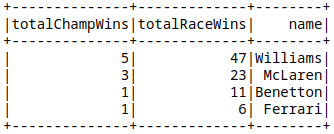
\includegraphics[scale=0.4]{results/constructordominance/90sconstructordominance.png}
	\centering
	\caption{Dominio de constructores en la década de los 90}
	\label{fig:constdominance}
	\centering
\end{figure}


Como se puede observar, el piloto más consistente es Fernando Alonso, con una diferencia entre las vueltas rápidas y todas las vueltas de la temporada de 1.461 segundos. Podemos ver también que el campeón de ese año, Sebastian Vettel queda en la parte baja de esta clasificación, con una diferencia al primero de casi 6 segundos.



% Fin del documento
\end{document}
